\documentclass[reprint,amsmath,amssymb,aps,pre,showkeys,showpacs]{revtex4-1}
% Latex
\usepackage[english]{babel}
\usepackage[utf8]{inputenc}
\usepackage[T1]{fontenc}
% Xelatex
%\usepackage{polyglossia}
%\usepackage{fontspec}
%\setdefaultlanguage{english}
%\setmainfont{DejaVu Sans}
%\setsansfont{DejaVu Sans}
%\setmonofont{DejaVu Sans Mono}
\usepackage{bm}
\usepackage{cleveref}
\usepackage{xcolor}
\usepackage{algpseudocode}
\usepackage{graphicx}
\usepackage{subfigure}
\usepackage[export]{adjustbox}

\definecolor{light-gray}{gray}{0.95}
\newcommand{\code}[1]{\colorbox{light-gray}{\texttt{#1}}}

\begin{document}
\preprint{APS/123-QED}

\author{Aleksei I. Samarin\textsuperscript{1,2}}
\author{Vasily Postnicov\textsuperscript{1}}
\author{Marina V. Karsanina\textsuperscript{1}}
\author{Efim V. Lavrukhin\textsuperscript{1,2}}
\author{Alexey N. Khlyupin\textsuperscript{1,3}}
\author{Kirill M. Gerke\textsuperscript{1}}
\email{kg@ifz.ru}

\affiliation{\textsuperscript{1}Schmidt Institute of Physics of the Earth of
  Russian Academy of Sciences, Moscow, 107031, Russia}
\affiliation{\textsuperscript{2}Computational Mathematics and Cybernetics,
  Lomonosov Moscow State University, Moscow, 119991, Russia}
\affiliation{\textsuperscript{3}Moscow Institute of Physics and Technology, 9
  Institutskiy per., Dolgoprudny, Moscow Region, 141701, Russia}

\title{Robust surface correlation functions evaluation from experimental
  discrete digital images}

\begin{abstract}
  Pore-scale modelling based on the 3D structural information of porous
  materials has enournous potential in assessing physical properties beyond the
  capabilities of laboratiry methods. Such capabilities are pricely in terms of
  computational expenses - this limits the applicability of the direct
  simulations to a small volume and requires high performance computational
  resources, espeically for multi-phase flow simulations. The only pore-scale
  technique capable of dealing with large representative volumes of porous
  samples is pore-network (PNM) based modelling. The problem of PNM approach is
  that 3D pore geometry first needs to be simplified into a graph of pores and
  throats that conserve topological and geometrical properties of the original
  3D image. While a lot of progress was achieved in terms of geometry
  representation, no methodology provides full conservation of the topological
  features of the pore structure.  In this paper we present a pore-network
  extraction algorithm for binary 3D images based on discrete Morse theory and
  persistent homology that by design targets topology preservation. In addition
  to methdological developments, we also clarify the relationship between
  topological characteristics of constructed Morse chain complex and
  pore-network elements. We show, that the Euler numbers calculated for PNMs
  based on our methodology coincide with those obtained using the direct
  topological analysis. The characteristics of extracted pore-network are
  calculated for several 3D porous binary images and compared with the results
  of maximum inscribed balls-based, watershed-based and hybrid approach to
  support our methdology.
\end{abstract}
\keywords {3D images; correlation functions; surface-surface function;
  surface-void function; image analysis; image scaling}

\maketitle

\section{Introduction}
Correlation functions (CFs) are invaluable universal descriptors of structure
and in this context are utilized in a multitude of scientific disciplines:
material sciences \cite{Cecen,chen2022quantifying}, rock
\cite{ledesma2018effect} and soil physics
\cite{Euras2012,PLoS_ONE,KarsaninaEJSS}, cosmology \cite{TakadaJain} and food
engineering \cite{Derossi2019}, to name just a handful. As such, CFs were used
to characterize the morphology \cite{tensorPRE} and representativeness via
correlation lengths \cite{vcapek2011transport,thovert2011grain}, compare
structures \cite{jiao2014chawla,EPL1,REVpaper}, compress structural information
\cite{SciRep1,Havelka,KarsaninaEJSS}, describe structural dynamics
\cite{chen2015dynamic,PLoS_ONE,xu2022correlation}, extract features for deep
learning \cite{Miao2017,kamrava2020linking,roding2020predicting,KarsaninaEJSS},
perform stochastic reconstructions
\cite{Adler_recon,Y-T,EPL2,tahmasebiPRL,karsaninaPRL} and fuse multi-scale
images \cite{SciRep1,chen2016stochastic,Geoderma2018}. Stochastic reconstruction
is a special topic of interest, as this approach allows to solve an inverse
problem and recover structure from a known set of correlation functions –- and
this ability for recovery is the basis for majority of potential usages in the
list above. Early reconstruction techniques mainly involved two-point
probability $S_2$ function, but were improved to include lineal $L_2$ function
\cite{Y-T,vcapek2009stochastic,vcapek2011transport}, cluster $C_2$ function
\cite{JiaoPNAS,jiao2014chawla} and potentially surface-surface $F_{ss}$
function. With the proper handling \cite{EPL2} it is possible to incorporate
numerous CFs into a reconstruction procedure. Increasing the number (and order)
of functions leads to higher information content of the CFs set
\cite{Gommes1,Gommes2}, thus, it allows to reconstruct and perform
stationarity/representativeness characterization \cite{REVpaper} for structures
of any complexity.

There are two ways to obtain correlation functions for a given structure at hand
-- either measure them experimentally with the help of scattering intensity
\cite{debye1957scattering,li2018accurate}, or measured from images. The first
approach suffers from the limitation of CFs that can be obtained this way
\cite{Gommes_notchord}, while the second one provides information with limited
resolution or/and resolution to field-of-view ratio \cite{SciRep1}. Moreover,
the most useful imaging methods such as X-ray computed tomography (XCT) and
scanning electron microscopy (SEM) due to their underlying physical principles
provide gray-scale images which, as we shall argue later on, need to be
segmented into constituent phases before CFs computation. It is important to
note that such gray-scale images do not represent spatial distribution of the
phases, but, for example, X-ray spatial attenuation or electron back-scattering
intensities. However, if properly segmented, high-resolution digital images do
provide a possibility to compute any correlation function. Experimental
measurements using small angle scattering (SAS) are traditionally used to
evaluate $S_2$, but it is also possible to relate scattering intensities to
surface correlation functions \cite{dietrich1995scattering,ma2018SS}. It would
be of great practical importance to obtain surface correlation functions from
both SAS and imaging (focused ion beam milling combined with SEM allows to
obtain the finest imaging resolution and sample CFs from
polished surfaces as opposed to surface imaging \cite{FIB-SEMpaper}) to estimate
coefficients for surface and bulk scattering (see Eq.13 in \cite{ma2018SS}). But
there is a catch -- SAS possesses close to infinite surface resolution as
opposed to digital pixelized images with inherent segmentation problems due to
partial volume effects, something we discuss extensively in this paper.

Recently, Ma and Torquato \cite{ma2018SS} laid foundation to precise surface
correlation function computations and showed the usefulness of these CFs
evaluation for numerous problems. They have implemented an elegant solution with
the help of infinite resolution random fields that (if the fields are
thresholded) allows finding an exact intersection with the sampling line. In
addition, they also showed that surface CFs for digital images can be computed
by converting integer fields (i.e., location of the phases) to float fields with
the help of Gaussian filter \cite{ma2018SS}. Unfortunately, their solution is
not readily applicable to the majority of grey-scale images due to
non-singularity in their chemical constitution. The reason is the difference
between the contour and real interface between different phases within the
material due to the partial volume effects \cite{Wildenschild_Sheppard} for XCT
imaging -- the presence of multiple phases within the same pixel/voxel. In other
words, the attenuation is a function of both density and atomic number, which
usually are distributed non-uniformly below the XCT imaging resolution. Somewhat
similar is also relevant for SEM imaging, as secondary or back-scattered
electrons are effectively a convolution of partial signals coming from different
depths \cite{Bultreys_review}. The exact sub-voxel thresholding based on
gray-scale image (similar to the technique used in \cite{ma2018SS}) is only
available in case it is monomineral, i.~e., the solid phase consists of a
completely chemically homogeneous substance that contrasts perfectly with
air/vacuum filled pore phase -- this is rarely the case for natural
materials. Moreover, even if the image of a monomineral sample (in natural
porouos media carbonate rocks can be considered monomineral depending on their
genesis) has sub-resolution features on XCT image, while it is possible to
compute the porosity of the voxel, it's still not possible to extract the
interface. All these and additional problems (such as, for example, experimental
noise and artifacts from inverse Radon transform) arising during gray-scale
image processing as related to image segmentation were extensively discussed
elsewhere \cite{NNseg}. In other words, simple thresholding of the grey-scale
image to compute surface functions using the approach proposed in
\cite{ma2018SS} (their section V.C) may result in inaccurate surface
identification and surface functions are not defined for grey-scale images (due
to possible sub-resolution porosity). Thus, we argue, that the usage of current
state-of-the-art segmentation techniques is necessary prior to the conversiton
to a coarse-grained scalar field. Moreover, finding an intersection between a
line segment and the countour is a computationally expensive procedure that
prevents on-the-fly application of surface functions. If a binary image
(consisting of pores and solids) is produced by adequate segmentation technique,
we still lack a robust and computationally effective procedure to evaluate
surface CFs from experimental XCT and SEM images of natural heterogeneous
materials, for instance, rocks and soils.

\begin{figure}[ht]
  \centering
  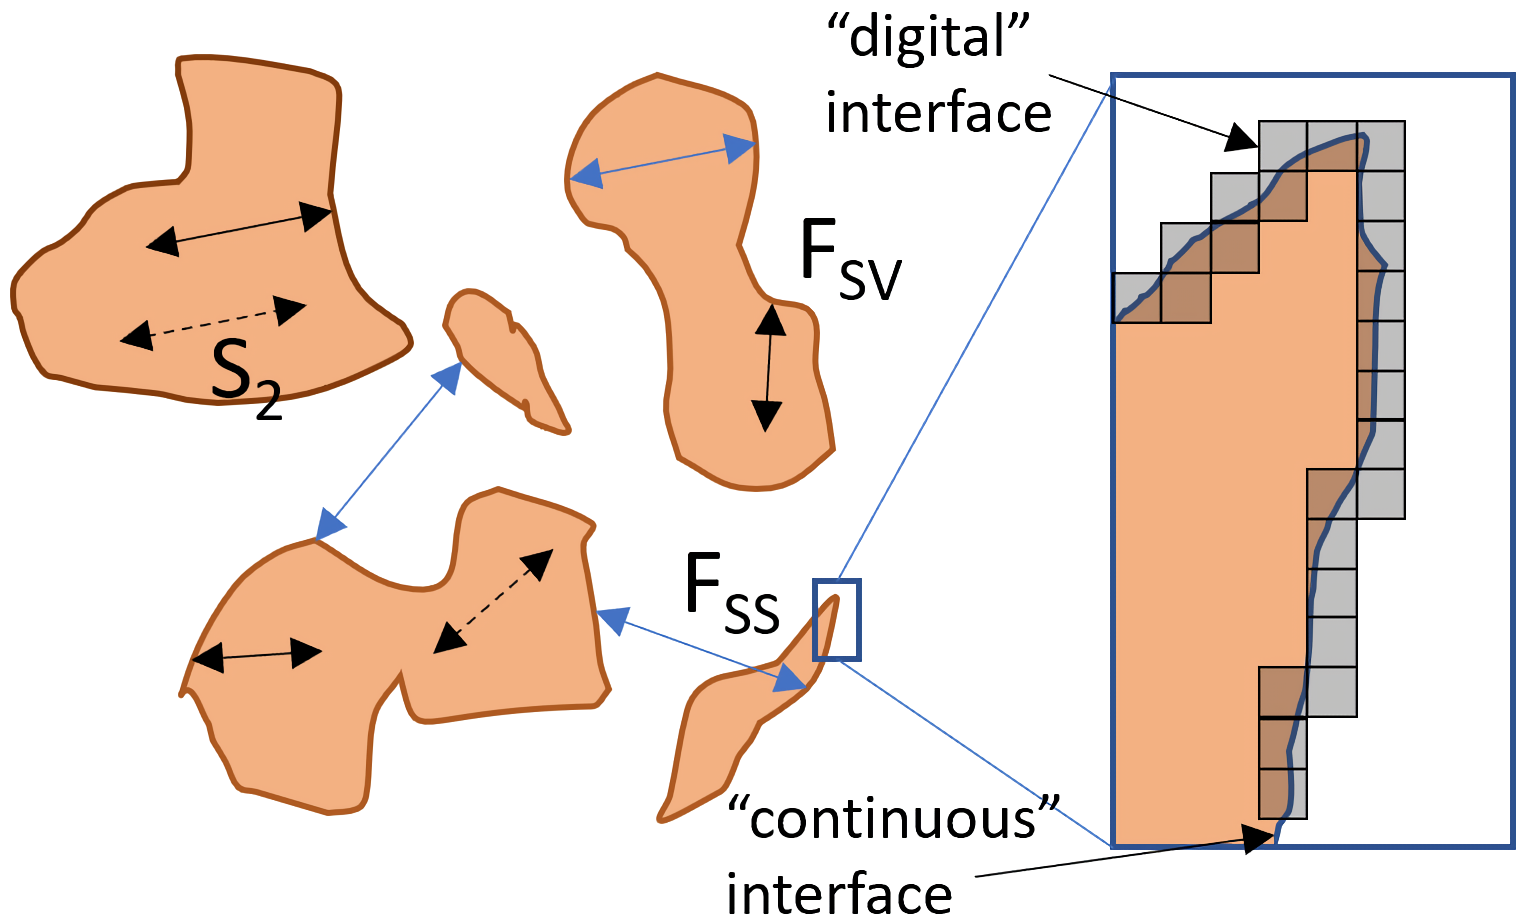
\includegraphics[width=\linewidth]{images/scheme.png}
  \caption[]{A schematic depiction of a binary porous media (pores are shown in
    color) with examples of positive events for surface $F_{ss}$, $F_{sv}$ and
    two-point probability $S_2$ correlation functions. The zoomed in area
    represents the difference between the true ``continuous'' interface in
    between pore and solid phases with pixelized ``digital'' interface emerging
    due to limited resolution of digital images.}
  \label{fig:scheme}
\end{figure}

To compute surface functions one first needs to elucidate the interface between
two phases (we shall consider only pores and solids, but, obviously, the
computations can be perfromed to multi-phase systems in the similar manner). The
interface area has infinitesimal volume, but its location on the digital image
is not easy due to the pixelization of the interface between the binary phases
\cite{ma2018SS}. By adopting the $\varepsilon$ = pixel/voxel size one can create
a very crude approximation of the real interface, but the usage of interfaces
between voxels ``as is'' leads to known problems in surface area and surface
geometry evaluation, in application of 3D imaging for geometry and topology
analysis \cite{AWR_PNM} or energy minimization problems
\cite{frank2018energy}. Another option would be to describe the boundaries
between voxels with some curves, e.~g., splines. This way it would be possible
to perform surface CFs sampling by line intersection as described by Ma and
Torquato \cite{ma2018SS}. While an exact boundary can be obtained for
deterministic structures such as disk/sphere packings, splines would provide
only a very approximate solution for the boundaries of arbitrary digitized
structure due to the limit in resolution for a given image
\cite{gerke2012tomographic}. In other words, contours extracted from digital
images will approach real boundaries between phases only when the spatial
resolution approaches infinity. But the same is also true for digital
pixelized/voxelized images. Thus, the options to compute surface correlation
functions include ``continuous'' approach (such as implemented in
\cite{ma2018SS}) and ``digital'' approach (similar to computation of $S_2$ from
digital images) as depicted in \cref{fig:scheme}. Here we propose a modified
``digital'' approach that lies in between the exact and pixelized solutions for
a number of reasons:
\begin{enumerate}
  \item For a binarized XCT or SEM image the interpolation of the interface
    using "continuous" or "digital" in the limit of $\varepsilon \to 0$ would
    produce the same results. Thus, as it is not possible to obtain the exact
    continuous interface from such an image, using "digital" approach is natural
    as applied to digital pixel/voxel images.
  \item "Continuous" approach is expensive numerically, as it requires to find the
    intersections between a line and a curve.
  \item Digital approach allows to utilize linear scan CFs computation or with
    the usage of the Fast Fourier Transform (FFT) - the latter is a fastest way
    to evaluate full CFs map and very efficient on modern GPUs.
\end{enumerate}

In this paper we build upon foundational work of Ma and Torquato \cite{ma2018SS}
and develop a robust and efficient approach to compute surface correlation
functions from digital 2D and 3D images. The rest of the manuscript is organized
as follows: in \cref{sec:details} we provide all methodological details for
surface CFs computation including analytical solutions to verify the proposed
methodology and describe an image library for extensive testing of our
algorithms, \cref{sec:results} presents all major results of surface functions
evaluations. We discuss obtained results, including the effects of image
scaling, and outline future uses of surface functions within
\cref{sec:outline}. The paper concludes with a summary in \cref{sec:summary}.

\section{Theoretical background}
\label{sec:theory}
\subsection{Correlation functions and definitions}
\label{sec:definitions}
Firstly, we introduce an indicator function $I^{(i)}(\mathbf{x})$ which marks
pixels of 2D and voxels of 3D digitized images as belonging to the phase $i$ or
not. It can be defined as:
\begin{equation*}
  I^{(i)}(\mathbf{x}) = \left\{
  \begin{array}{ll}
    1 & \quad \mathbf{x} \in V_i \\
    0 & \quad \text{otherwise}
  \end{array}
  \right.
\end{equation*}
where $V_i \subset \mathbb{R}^n$ is the region occupied by phase $i$. For
statistically homogeneous media the ensemble average of $I^{(i)}$ equals volume
fraction of a given phase. For binary media the following equality holds:
\begin{align*}
  \phi_{void} &+ \phi_{solid} = 1 \\
  \phi_i &= \langle I^{(i)}(\mathbf{x}) \rangle
\end{align*}
In a similar fashion we can define an interface indicator function
$M(\mathbf{x})$ which provides interface area $s$ if averaged over the whole
image:
\begin{align}
  M(\mathbf{x}) = |\nabla I^{(solid)}(\mathbf{x})| &= |\nabla I^{(void)}(\mathbf{x})|
  \label{eq:interface} \\
  \langle M(\mathbf{x}) \rangle &= s
  \label{eq:surface}
\end{align}
The simplest, yet foundational correlation function is the two-point probability
function $S_2$ which is defined as a probability that the ends of a random line
segment belong to the same phase:
\begin{equation}
  S_2^{(i)}(\mathbf{x}_1, \mathbf{x}_2) = \langle I^{(i)}(\mathbf{x}_1)
  I^{(i)}(\mathbf{x}_2) \rangle \label{eq:twopoint}
\end{equation}
This equation can be further simplified for statistically homogeneous media, as
$S_2$ will dependent only on the relative displacement $\mathbf{r}$:
\begin{equation*}
  S_2^{(i)}(\mathbf{x}_1, \mathbf{x}_2) = S_2^{(i)}(\mathbf{r})
\end{equation*}
The value of $S^{(i)}_2(\mathbf{r})$ at $\mathbf{r} = 0$ is a fraction of phase
$i$ in a medium:
\begin{equation*}
  S_2^{(i)}(0) = \phi_i
\end{equation*}
For isotropic media a vector displacement $\mathbf{r}$ can be replaced with its
length $r = |\mathbf{r}|$ and $S_2(\mathbf{r})$ with $S_2(r) = S_2(|\mathbf{r}|)$.
Now, analogously to $S_2$ we can define surface-surface and surface-void
correlation functions (for homogeneous and isotropic media straight away):
\begin{align}
  F_{ss}(r) &= \langle M(x)M(x+r) \rangle \label{eq:fss} \\
  F_{sv}(r) &= \langle M(x)I^{(void)}(x+r) \label{eq:fsv} \rangle
\end{align}

The interface indicator function $M(x)$ is basically defined as infinity on the
interface and zero elsewhere. Therefore, it is hard to directly compute
$\langle M(x), M(x + r) \rangle$. We can replace the line of zero width and infinite value
with a strip of width $\varepsilon$ and value $\frac{1}{\varepsilon}$: $M(x; \varepsilon)$.
Then $F_{ss}(x; \varepsilon) = \langle M(x; \varepsilon), M(x + r; \varepsilon) \rangle$
is simply an intersection area of two strips -- original and shifted --
multiplied by $(\frac{1}{\varepsilon})^2$.
And with $\varepsilon \to 0 \Rightarrow F_{ss}(r; \varepsilon) \to F_{ss}(r)$.
Area between two black dashed circles on \cref{fig:Fss-explained} represents
$M(x; \varepsilon)$, red is for $M(x + r; \varepsilon)$. Blue color marks the
intersection area. More detailed information on two-point probability and
surface correlation functions can be found in comprehensive Torquato's book
\cite{Torquato_book}.

\begin{figure}
  \centering
  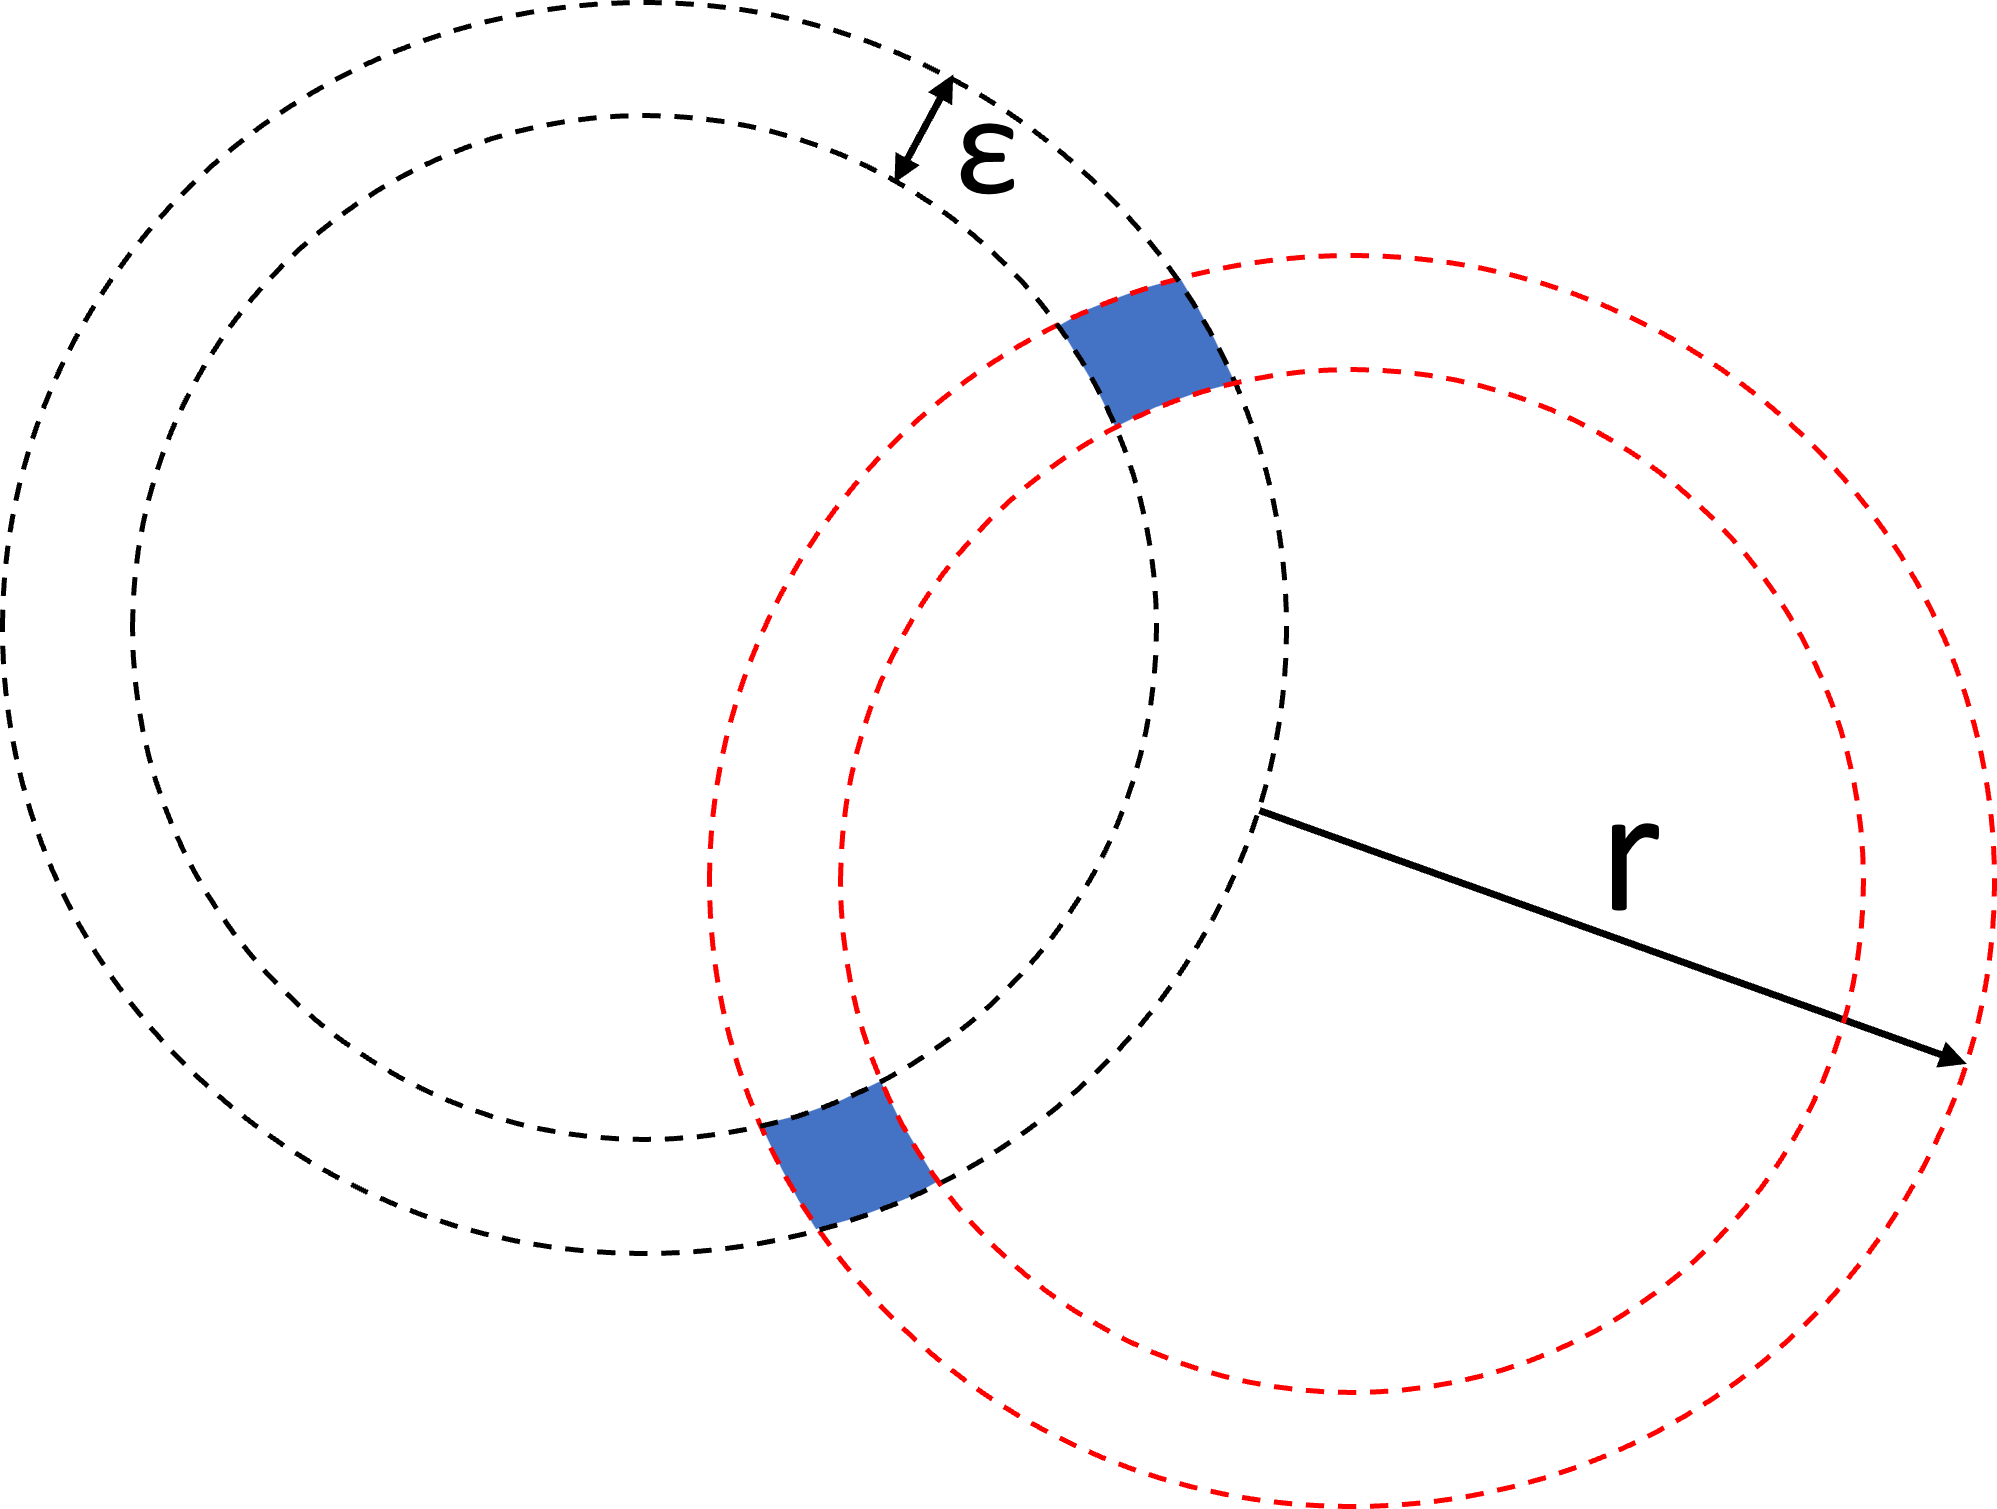
\includegraphics[width=\linewidth]{images/Fss.png}
  \caption[]{Interpretation of $F_{ss}$ as self-intersection of the interface.}
  \label{fig:Fss-explained}
\end{figure}

\subsection{Analytical solutions}
For Poisson disks and balls one can derive exact analytical surface-surface and
surface-void functions. For overlapping disks with radius $R$ and centers
generated by Poisson point process with parameter $\lambda$ we have (see the
derivation of these formulas in \cref{ap:overlapping-disks}):
\begin{align}
  F_{sv}(r) &= S_2(r) \left\{
  \begin{array}{ll}
    2(\pi - B)R \lambda & \quad r<2R \\
    2\pi R \lambda & \quad \text{otherwise}
  \end{array} \right. \label{eq:fsv_final} \\
  F_{ss}(r) &= S_2(r) \left\{
  \begin{array}{ll}
    \frac{(2(B-\pi)R\lambda)^2Ar + 4\sqrt{A}R^2\lambda}{Ar} & \quad r<2R \\
    (2\pi R\lambda)^2 & \quad \text{otherwise},
  \end{array} \right. \label{eq:fss_final}
\end{align}
where $S_2$ is the regular two-point correlation function and
\begin{align*}
  A &= 4R^2 - r^2 \\
  B &= \arccos(\frac{r}{2R}).
\end{align*}

For 3D balls the relationships are readily available in the literature
\cite{Torquato_book,ma2018SS}:
\begin{align*}
  F_{sv}(r) &= S_2(r) \left\{
  \begin{array}{ll}
    4\pi R^2\lambda(\frac{1}{2} + \frac{r}{4R}) & \quad r<2R \\
    4\pi R^2\lambda & \quad \text{otherwise}
  \end{array} \right. \\
  F_{ss}(r) &= S_2(r) \left\{
  \begin{array}{ll}
    {(4\pi R^2 \lambda (\frac{1}{2} + \frac{r}{4R}))^2 + \frac{2\pi R^2 \lambda}{r}} & \quad r<2R \\
    (4\pi R^2 \lambda)^2 & \quad \text{otherwise}.
  \end{array} \right.
\end{align*}

These analytical solutions will be used to verify the accuracy of our evaluation
of surface CFs for such systems.

\section{Methodological details}
\label{sec:details}
By looking at \cref{eq:twopoint,eq:fss,eq:fsv} one can observe
some significant similarities between two-point probability and two-point
surface functions (see \cref{fig:scheme}). $S_2$ can be viewed as a
autocorrelation of the image, i.~e., computing correlations between shifted
realization of the image -- something that can be used to effectively compute
$S_2$ with the help of the FFT on modern hardware, especially GPUs. If we apply
the same analogy to $F_{ss}$, \cref{eq:fss} can be considered as an intersection
of the interface with itself for all possible shifts. Recall that for the
correlation length of zero this intersection is technically infinity
(\cref{sec:definitions}). While surface-void function is well defined at $r=0$,
it differs from $S_2$ in two significant aspects. Firstly, it resembles two-point
cross-correlation function (as instead of autocorrelation we have to compute
correlation between the interface and the void phase). Secondly, such
cross-correlation is not commutative, so we get two surface-void functions:
correlation between an interface and a void phase and correlation between a void
phase and an interface. These considerations will be very useful in
understanding of our computational framework as described in this section.

\subsection{The general algorithm}
\label{sec:general}
While we present and compare a bunch of sligtly different methods to evaluate
surface CFs, they are all based on a single general algorithm for each surface
function as desribed below ($A$ refers to the input 2D or 3D digital image, $M$
is the interface between two phases, and $V$ is the image of the void phase only):

$F_{ss}$ algorithm:
\begin{algorithmic}[1]
  \Procedure{surfsurf}{$A, i$}
  \State $A' \gets I^{(i)}(A)$
  \Comment{Apply indicator function to $A$.}
  \State $M \gets M(A')$
  \Comment{Extract interface from $A'$.}
  \State \textbf{return} $\star(M, M)$
  \Comment{Autocorrelation of $M$.}
  \EndProcedure
\end{algorithmic}

$F_{sv}$ algorithm:
\begin{algorithmic}[1]
  \Procedure{surfvoid}{$A, i$}
  \State $A' \gets I^{(i)}(A)$
  \Comment{Apply indicator function to $A$.}
  \State $M \gets M(A')$
  \Comment{Extract interface from $A'$.}
  \State $V \gets I^{(void)}(A')$
  \Comment{Extract void phase from $A'$.}
  \State \textbf{return} $\star(M, V)$
  \Comment{Cross-correlation of $M$ and $V$.}
  \EndProcedure
\end{algorithmic}

The algorithm is very general and allows to utilize different technques for
interface extraction or computation of the correlations, as detailed below. The
cross-correlation function is introduced in \cref{sec:cross-comp}. Consecutive
stages of our method are shown in \cref{fig:stages}. It is also a part of
\code{CorrelationFunctions.jl} package \cite{CFsjlpaper} for Julia programming
language that allows to compute all classical CFs described in Torquato’s book
\cite{Torquato_book} from digital images.

\subsection{Interface extraction}
We shall consider two methods for the interface extraction -- the first one is a
naive approach, while the second is the one we propose to apply for XCT and SEM
images.

\begin{figure}
  \centering 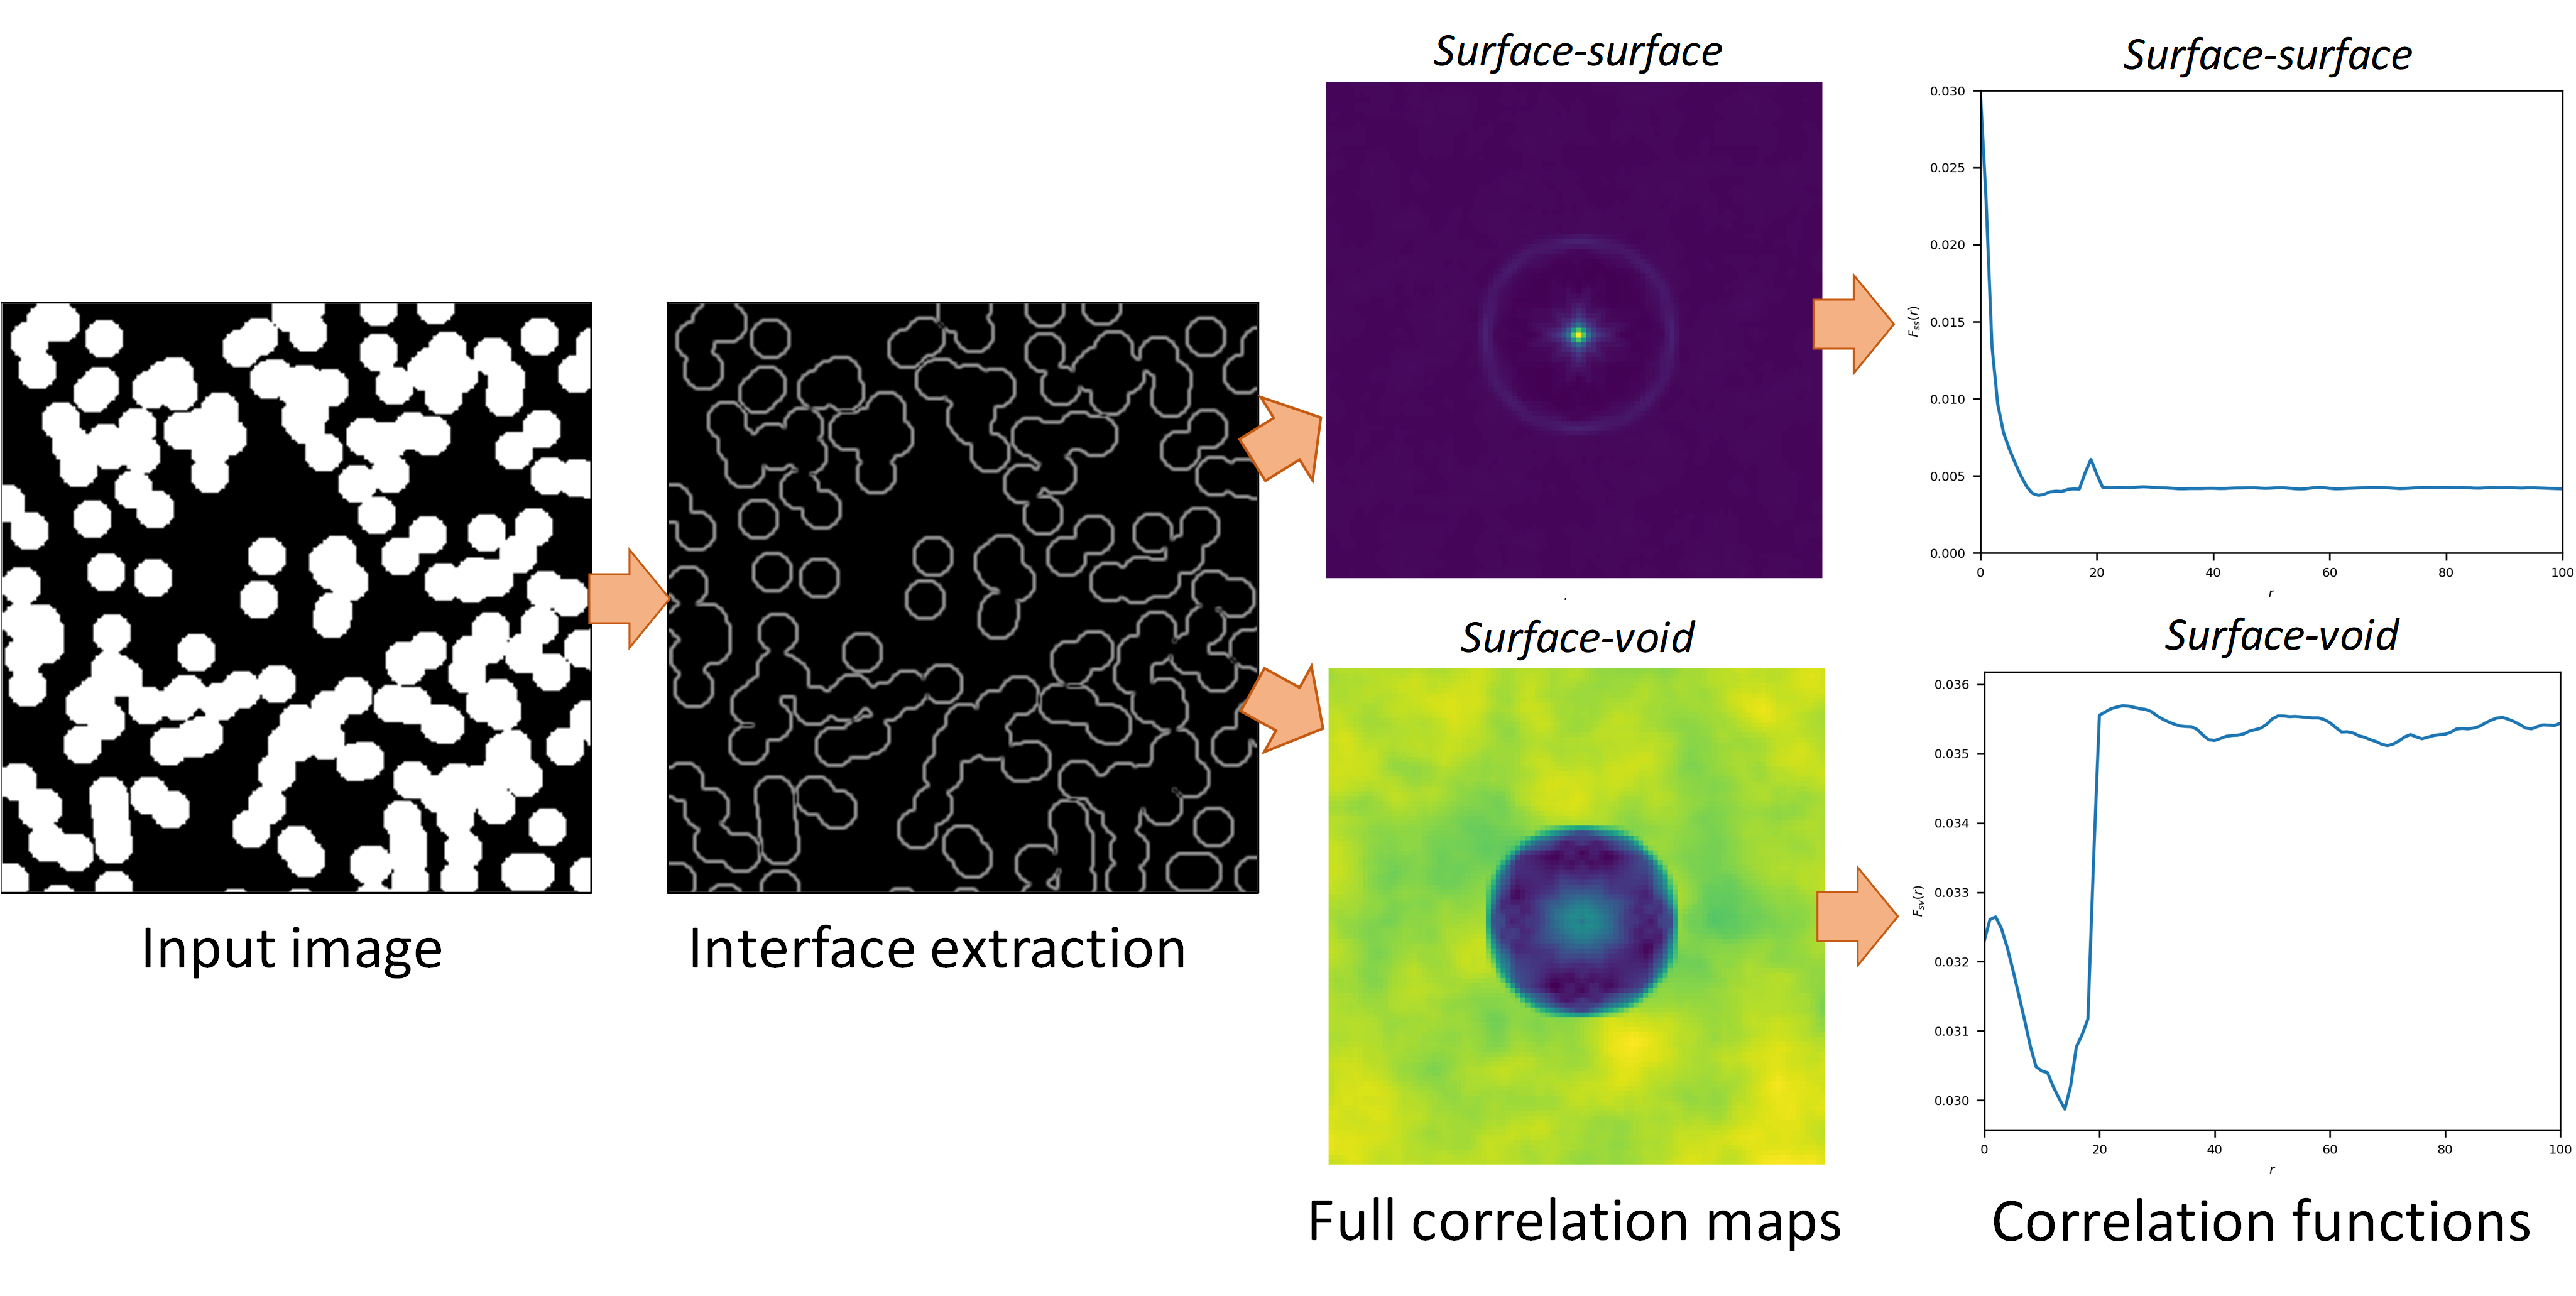
\includegraphics[width=\linewidth]{images/algo.png}
  \caption{Schematic example of the algorithm for computation of surface
    functions (2D case is considered for visibility). \textcolor{red}{I need to
      re-work this one, need original images from Vasya (Kirill).}}
  \label{fig:stages}
\end{figure}

\textit{Distance map}.
One solution to extract an interface between phases from an image is to use the
distance map (also called the distance transform). Distance transform is a
mapping from a binary image to a scalar field using one of the following
functions:
\begin{align}
  D_{o}(\mathbf{x}) &= \left\{
  \begin{array}{ll}
    0 & \quad \mathbf{x} \in V_{void} \\
    \min \rho(\mathbf{x}, \mathbf{y}) \ \forall \mathbf{y} \in V_{void} & \quad \text{otherwise}
  \end{array}
  \right. \label{eq:dist-outer} \\
  D_{i}(\mathbf{x}) &= \left\{
  \begin{array}{ll}
    0 & \quad \mathbf{x} \not\in V_{void} \\
    \min \rho(\mathbf{x}, \mathbf{y}) \ \forall \mathbf{y} \not\in V_{void} & \quad \text{otherwise}
  \end{array}
  \right. \label{eq:dist-inner}
\end{align}
where $V_{void}$ is a set containing elements belonging to the void phase and
$\rho(\mathbf{x}, \mathbf{y})$ is the Euclidean distance between points
$\mathbf{x}$ and $\mathbf{y}$. Now $M(\mathbf{x})$ in \cref{eq:interface} may be
written as follows:
\begin{equation*}
  M(\mathbf{x}) = \left\{
  \begin{array}{ll}
    1 & 0 < \quad D(\mathbf{x}) \le \sqrt{d} \\
    0 & \quad \text{otherwise}
  \end{array}
  \right.
\end{equation*}
where $d$ is dimensionality of the image ($d = 2$ for 2D image, $d = 3$ for 3D
image) and $D(\mathbf{x})$ is evaluated using either \cref{eq:dist-outer} or
\cref{eq:dist-inner}. When $D = D_i$ we call the resulting interface
``the inner interface'' and when $D = D_o$ we call it ``the outer interface''.

\textit{Image filtering}.  This method creates a grayscale image of the
interface with the help of the edge-detecting filter. We use Sobel operator $S$
to detect edges of the image (other edge detecting filters are also considered,
see below), so $M = S$ in algorithms in \cref{sec:general}. We calculate
$\|S(A')\|$ (recollect that $A' = I^{(void)}(A)$ where $A$ is the input image)
element-wise ($\|\cdot\|$ denotes the usual norm on Euclidean space). This norm
can be interpreted as the probability that a point in $A$ belongs to the
interface. In a digitized image $\|S(A')\|$ can be represented as an array of
floating point numbers having the same shape as an original image $A$.

\subsection{Computing correlation}
\label{sec:cross-comp}
Let us now describe the approach for the computation of cross-correlation
function between two images $f$ and $g$. In the case of autocorrelation function
we assume $f = g$. Algorithm is straightforward when boundary conditions are
periodic. For non-periodic boundary conditions we need some additional
modifications.

\textit{Periodic boundary condition}
\begin{algorithmic}[1]
  \Procedure{$\star$}{$f, g$}
  \State $\hat{f} = F(f)$
  \State $\hat{g} = F(g)$
  \Comment Compute FFT of the input.
  \State $\hat{cc} \gets \hat{f} \cdot \overline{\hat{g}}$
  \Comment Multiply element-wise.
  \State $cc \gets F^{-1}(\hat{cc})$
  \Comment Compute IFFT of $\hat{cc}$.
  \State \textbf{return} $cc$ divided by the number of pixels in the input.
  \EndProcedure
\end{algorithmic}

\textit{Non-periodic boundary condition}
\begin{algorithmic}[1]
  \Procedure{$\star$}{$f, g$}
  \State Pad $f$ and $g$ with zeros in each dimension to the size $2n-1$ where
  $n$ is the size of the image in that dimension.
  \State $\hat{f} = F(f)$
  \State $\hat{g} = F(g)$
  \Comment Compute FFT of the input.
  \State $\hat{cc} \gets \hat{f} \cdot \overline{\hat{g}}$
  \Comment Multiply element-wise.
  \State $cc \gets F^{-1}(\hat{cc})$
  \Comment Compute IFFT of $\hat{cc}$.
  \State circle shift $cc$ by $n - 1$ in each direction, so index range becomes
  from $-(n - 1)$ to $n - 1$.
  \State $cc_{ij} \gets cc_{ij} / q_{ij}$ where $q_{ij} = (n - |i|)(m - |j|)$
  \Comment Divide each element $cc_{ij}$ by the number of pixels whose
  coordinate difference is equal to $(i, j)$.
  \State \textbf{return} $cc$.
  \EndProcedure
\end{algorithmic}

The results of the computations are a full correlation map. To obtain the
ensemble averaged surface correlation functions one just needs to convert the
map to CF vs. $r$ relationship. This is also possible to compute directional
surface CFs in this manner in case the structure at hand is anisotropic. Without
loss of generality, $\star$($f, g$) can be also computed by scanning with the
line segment of length $r$, but this approach is more efficient on CPU as
compared to GPU implementation here. If not stated othwerwise, we report the
ensemble averaged functions computed from the full map (assuming the isopropy of
the input image). One can easily compute directional CFs
\cite{jiao2014chawla,EPL1} using both segment scanning or from correlation maps.

\section{Application to synthetic images, veryfication and betterment of the methodology}
\label{sec:results}
\subsection{Comparisons against analytical solutions}
\label{sec:comparison}
To evaluate the accuracy of surface CFs computations the most straightforward
way is to compare them against analytical solutions. We use classical
analytical soulutions for overlapping disks and balls with fixed radius $R$ and
centers generated by Poisson point process with parameter $\lambda$. Starting
with an image with resolution of $4096 \times 4096$ pixels, we then downscale it
by 4, 16, and 64 times with the help of bicubic interpolation
\cite{ledesma2018effect} (see \cref{fig:disks-noise}). We show that calculated
correlation functions approach theoretical values when the resolution is high
enough.
\begin{figure*}[t]
  \centering
  \subfigure[Image size $4096 \times 4096$, disk radius 61.44 pixels, $C_{0.5} = 0.9593$]{
    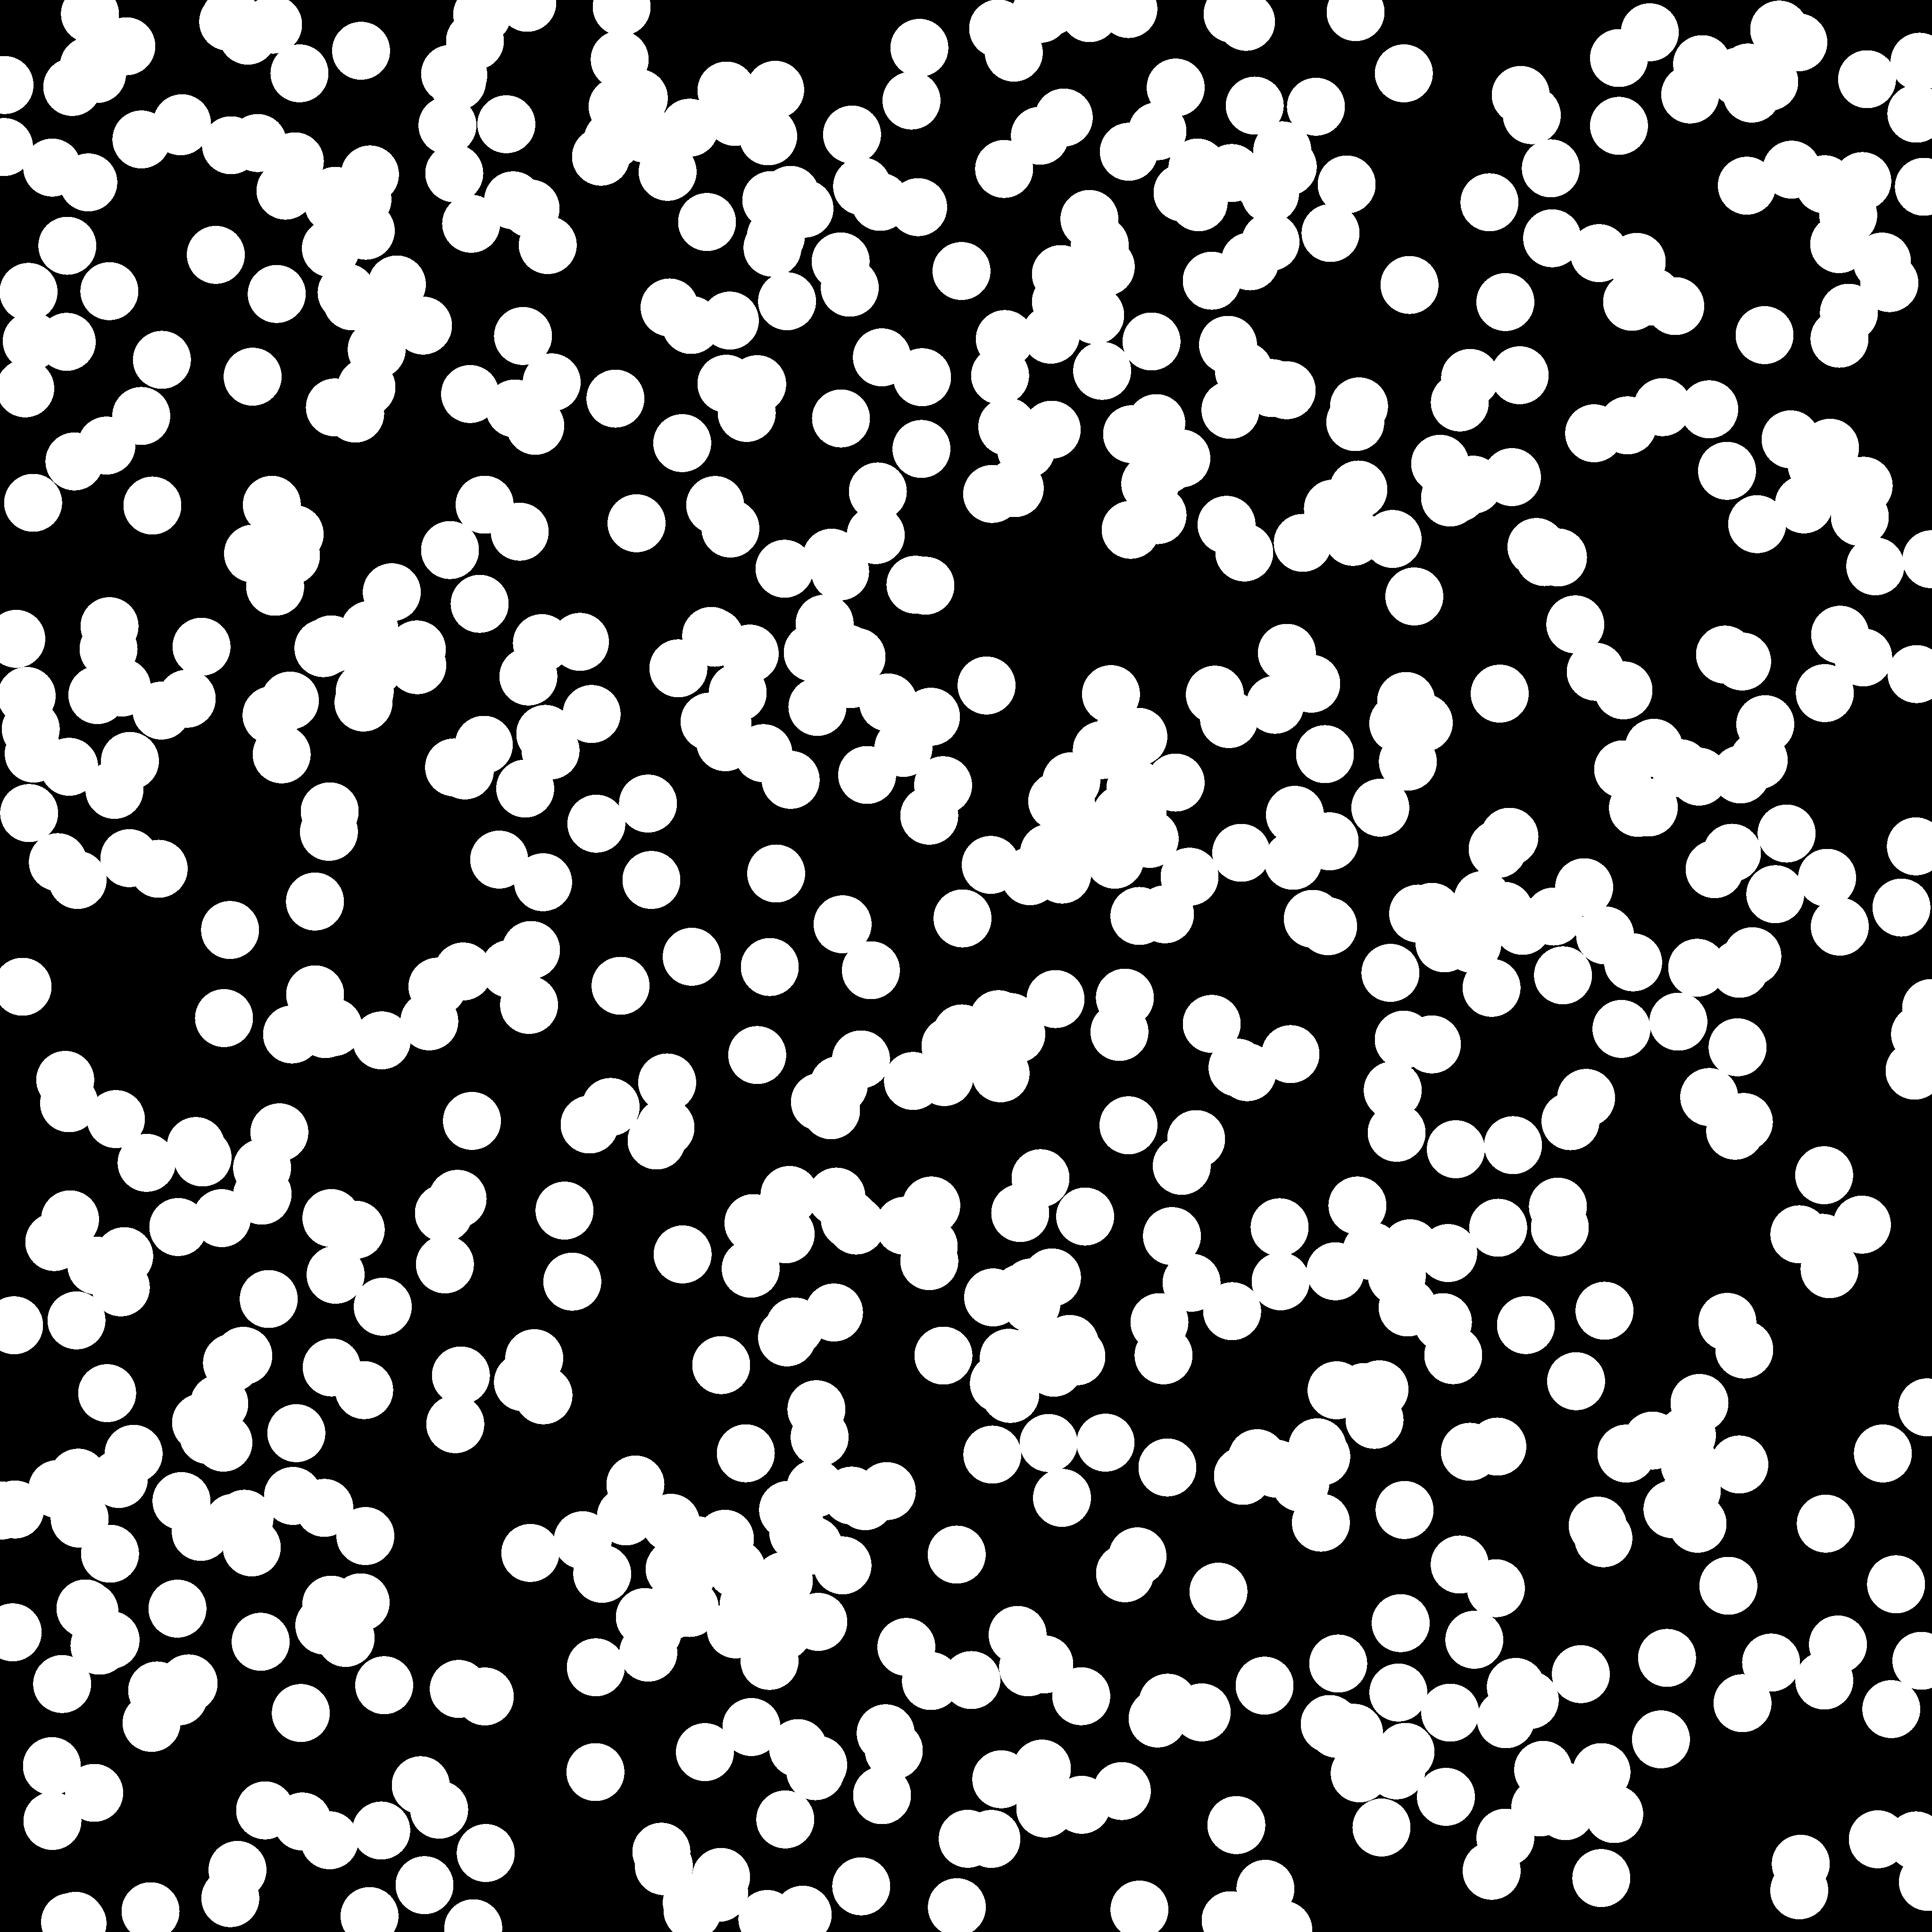
\includegraphics[width=0.22\linewidth, frame]{images/disks-0015-5e-5-4096.png}
    \label{fig:disks-4096}}
  \hfill
  \subfigure[Image size $1024 \times 1024$, disk radius 15.36 pixels, $C_{0.5} = 0.9185$]{
    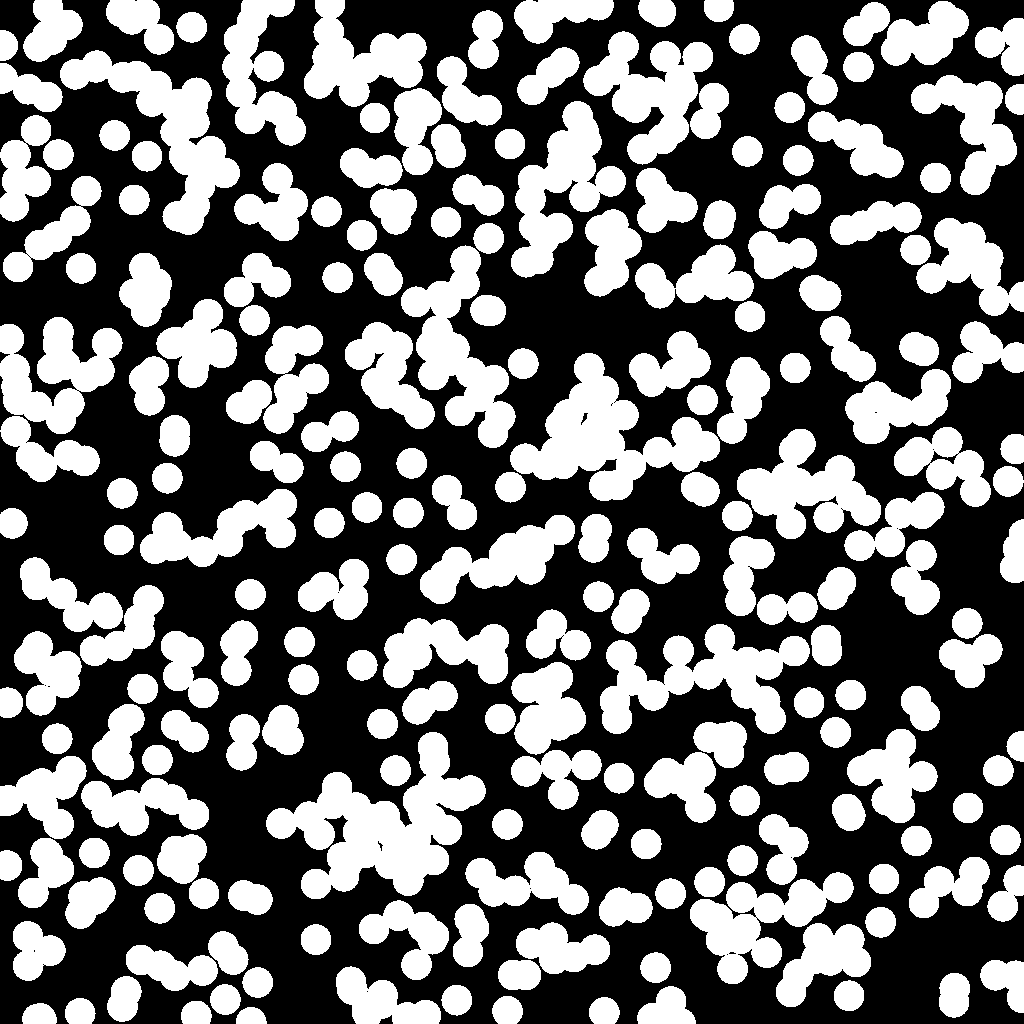
\includegraphics[width=0.22\linewidth, frame]{images/disks-0015-5e-5-1024.png}
    \label{fig:disks-1024}}
  \hfill
  \subfigure[Image size $256 \times 256$, disk radius 3.84 pixels, $C_{0.5} = 0.8356$]{
    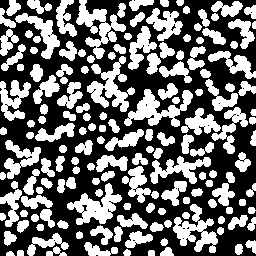
\includegraphics[width=0.22\linewidth, frame]{images/disks-0015-5e-5-256.png}
    \label{fig:disks-256}}
  \hfill
  \subfigure[Image size $64 \times 64$, disk radius 0.96 pixels, $C_{0.5} = 0.6549$]{
    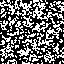
\includegraphics[width=0.22\linewidth, frame]{images/disks-0015-5e-5-64.png}
    \label{fig:disks-64}}
  \vskip\baselineskip
  \subfigure[Image size $4096 \times 4096$, value noise, $C_{0.5} = 0.9692$]{
    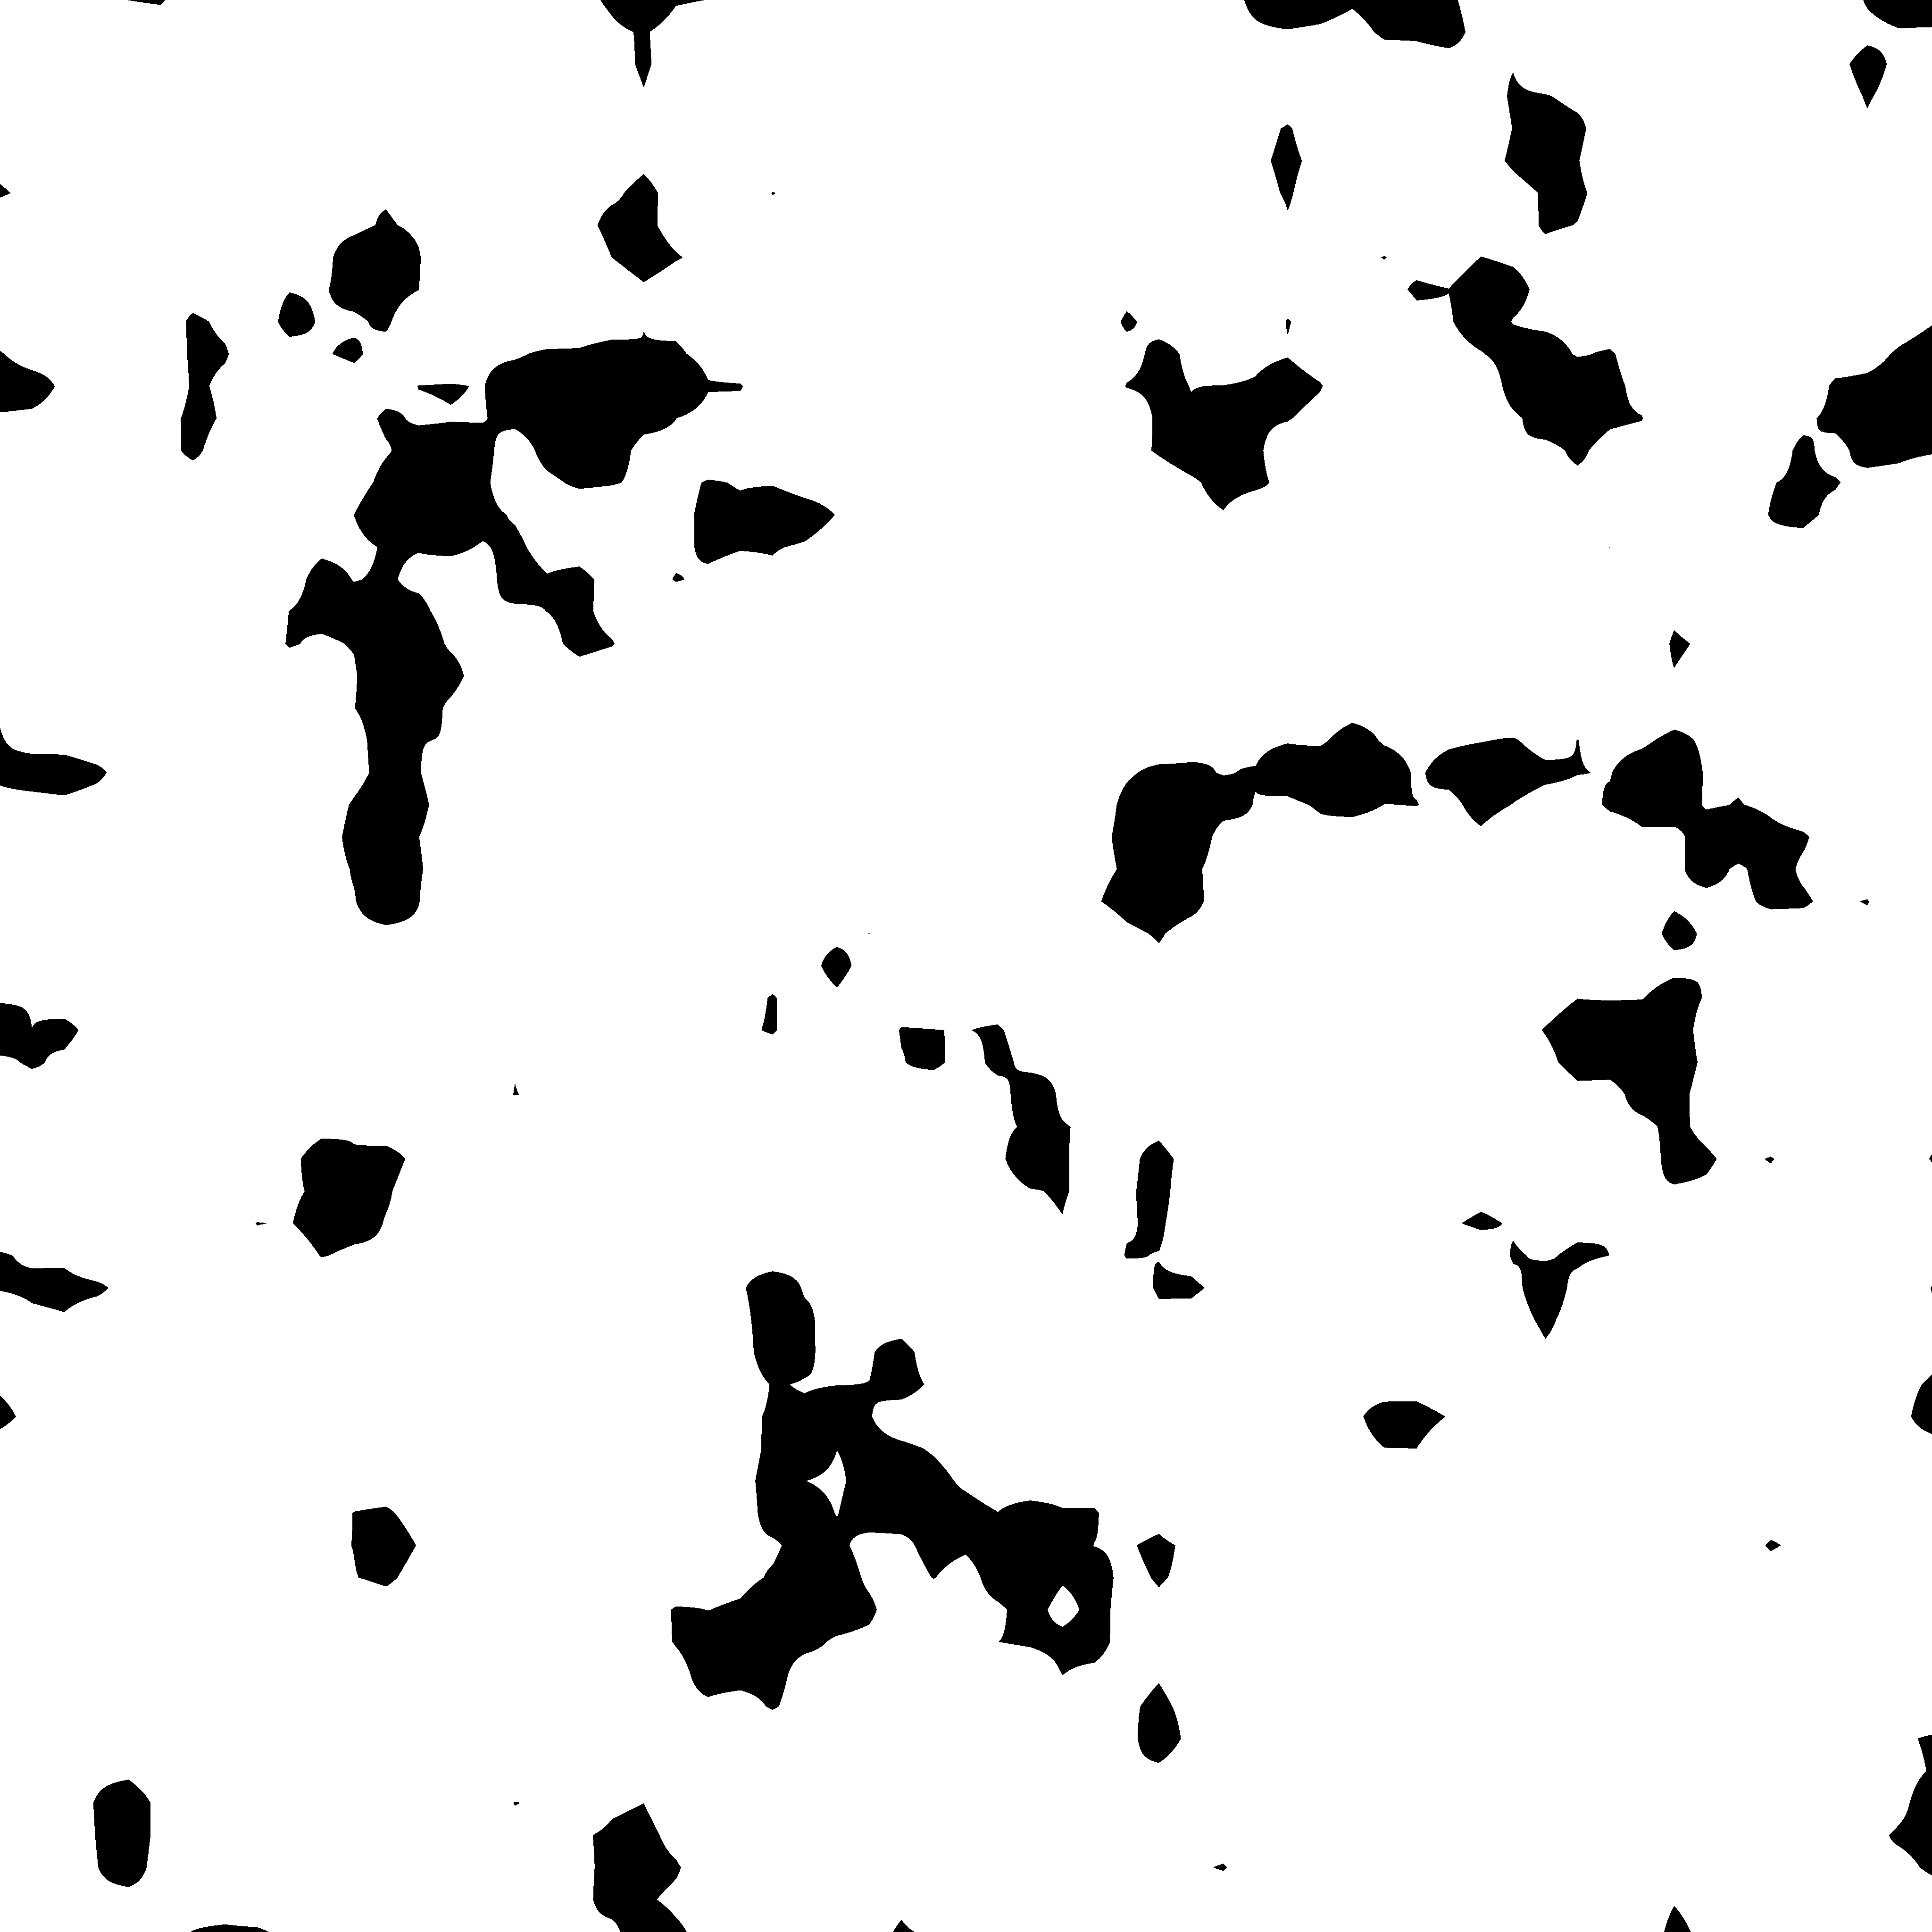
\includegraphics[width=0.22\linewidth, frame]{images/noise-4096.png}
    \label{fig:noise-4096}}
  \hfill
  \subfigure[Image size $1024 \times 1024$, value noise, $C_{0.5} = 0.9386$]{
    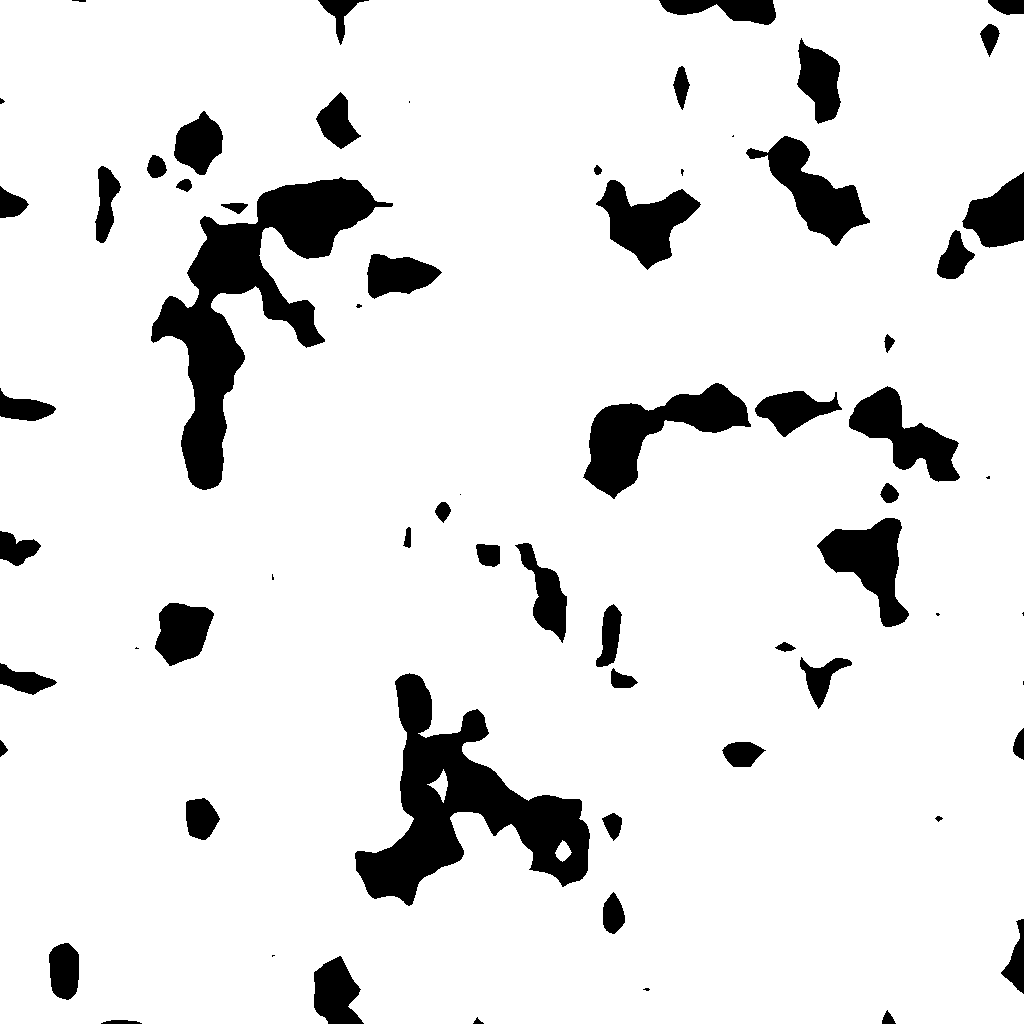
\includegraphics[width=0.22\linewidth, frame]{images/noise-1024.png}
    \label{fig:noise-1024}}
  \hfill
  \subfigure[Image size $256 \times 256$, value noise, $C_{0.5} = 0.8770$]{
    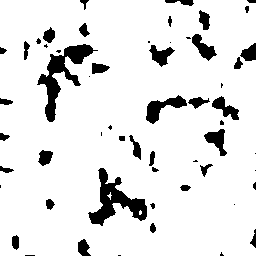
\includegraphics[width=0.22\linewidth, frame]{images/noise-256.png}
    \label{fig:noise-256}}
  \hfill
  \subfigure[Image size $64 \times 64$, value noise, $C_{0.5} = 0.7524$]{
    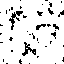
\includegraphics[width=0.22\linewidth, frame]{images/noise-64.png}
    \label{fig:noise-64}}
  \caption[]{2D images of overlapping disks (a-d) and value noise (e-h) with
    different resolution (\cref{sec:results}).}
  \label{fig:disks-noise}
\end{figure*}

It is easy to show that for $a > 0$:
\begin{align}
  a^2 F_{ss}(a \mathbf{x}, a(\mathbf{x} + \mathbf{r})) &= F_{ss}(\mathbf{x},
  \mathbf{x} + \mathbf{r}) \label{eq:scale-ss} \\
  a F_{sv}(a \mathbf{x}, a(\mathbf{x} + \mathbf{r})) &= F_{sv}(\mathbf{x},
  \mathbf{x} + \mathbf{r}) \label{eq:scale-sv}
\end{align}
Assuming that our images represent homogeneous and isotropic media, we calculate
$F_{ss}(ar)$ and $F_{sv}(ar)$ for each original and rescaled image and multiply
it by coefficient $a^2 = (L_{scaled}/L_{orig})^2$ and $a = L_{scaled}/L_{orig}$
respectively, where $L_{scaled}$ is the side of the rescaled image and
$L_{orig}$ is the side of the original image. The resulting scaled surface CFs
are shown in \cref{fig:scaling-alltogether}.

\begin{figure*}[ht]
  \centering
  \subfigure[Surface-surface, disks]{
    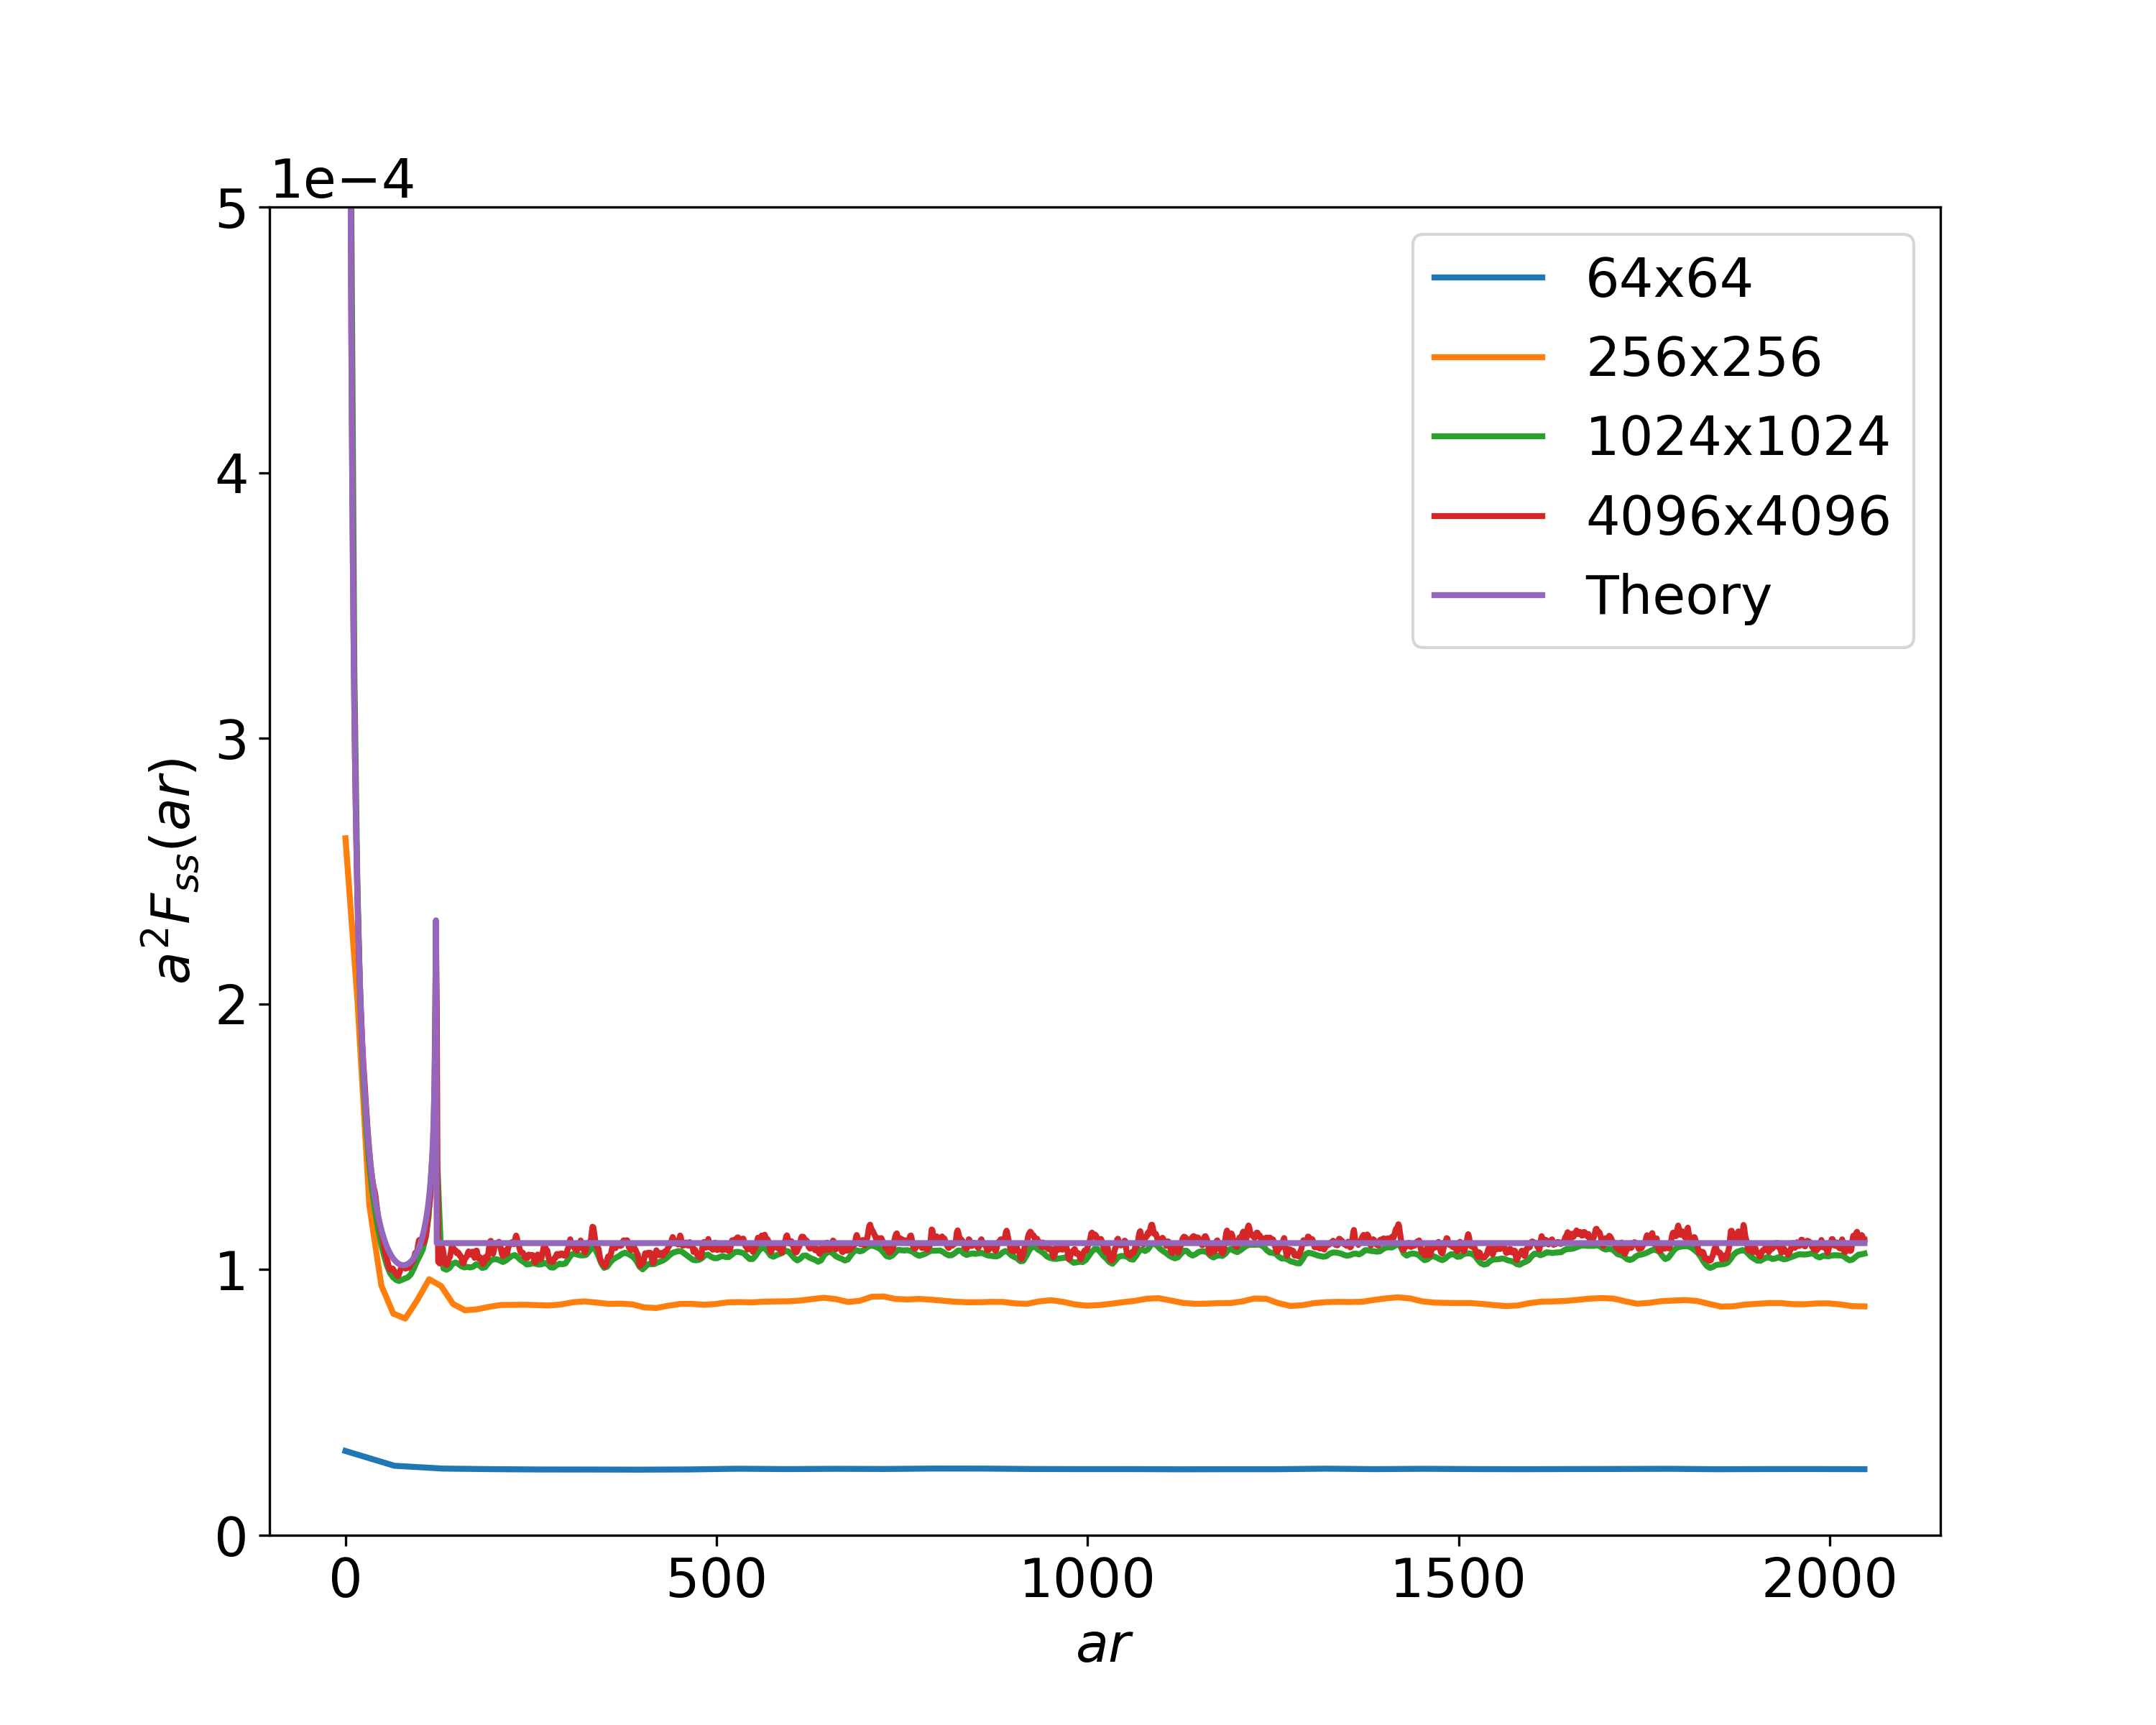
\includegraphics[width=0.475\linewidth]{images/plot-ss-balls.png}
    \label{fig:fss-scaling}}
  \hfill
  \subfigure[Surface-void, disks]{
    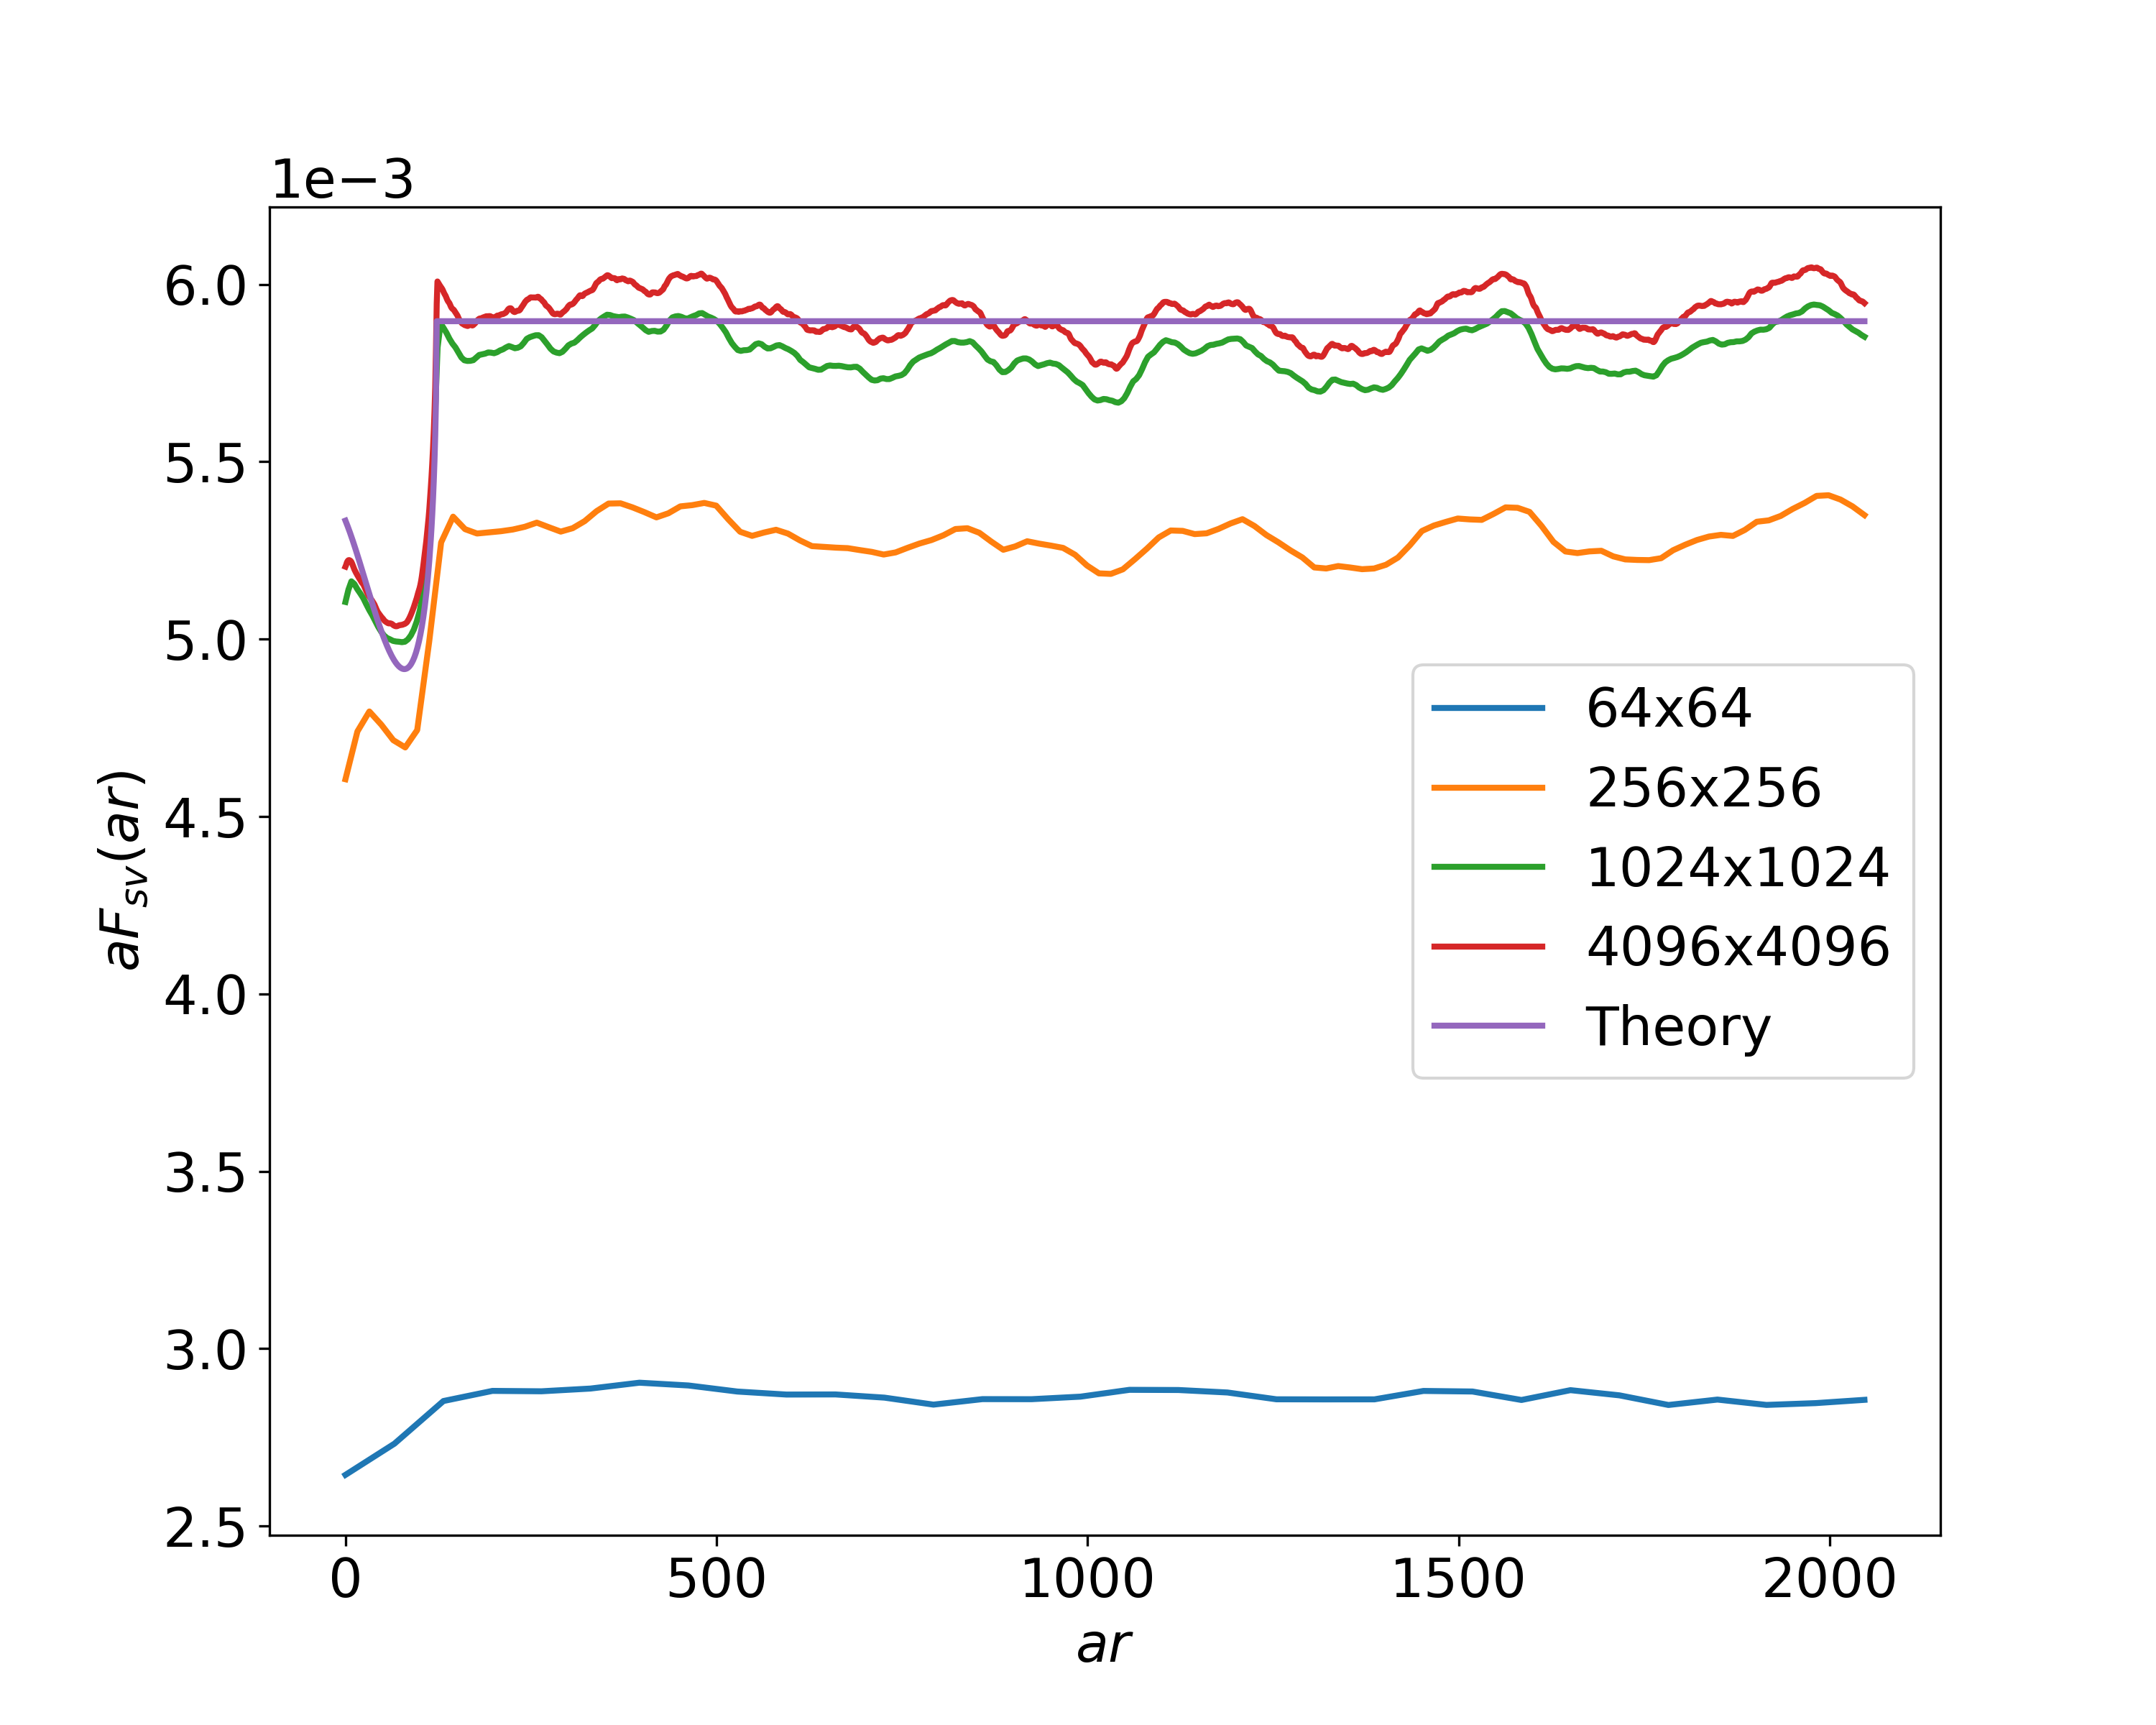
\includegraphics[width=0.475\linewidth]{images/plot-sv-balls.png}
    \label{fig:fsv-scaling}}
  \vskip\baselineskip
  \subfigure[Surface-surface, value noise]{
    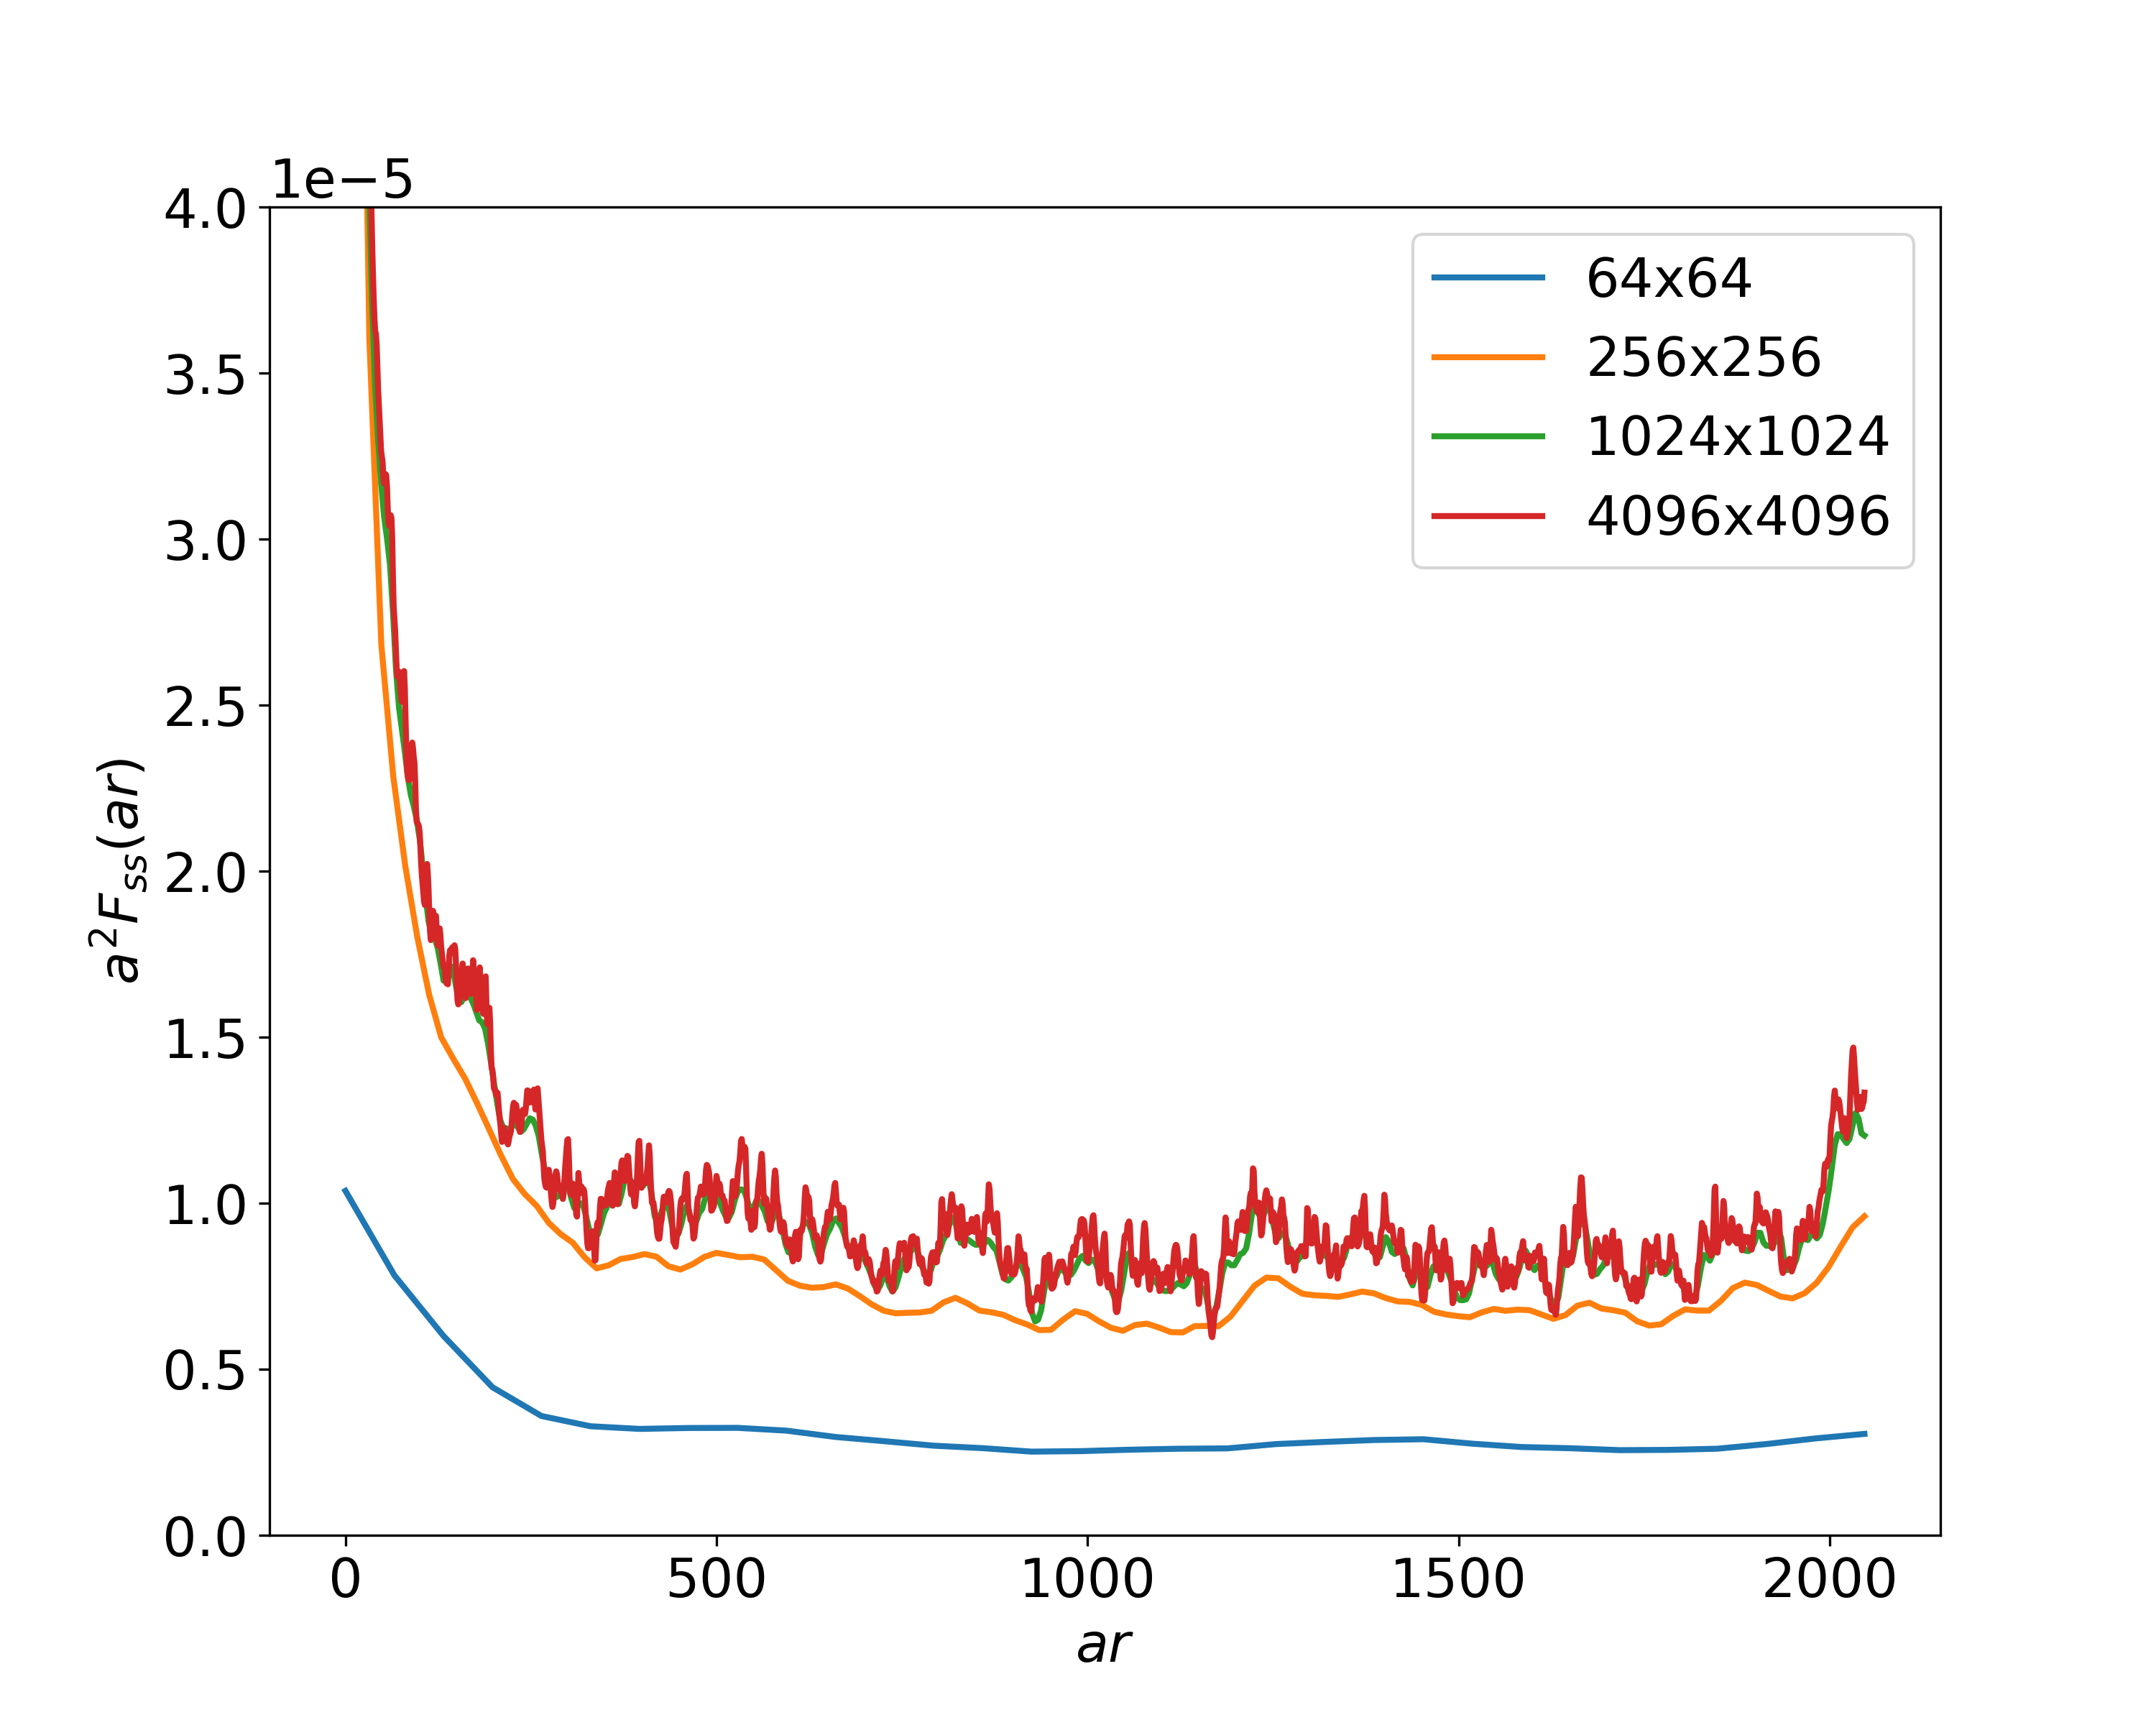
\includegraphics[width=0.475\linewidth]{images/plot-ss-noise.png}
    \label{fig:fss-scaling-noise}}
  \hfill
  \subfigure[Surface-void, value-noise]{
    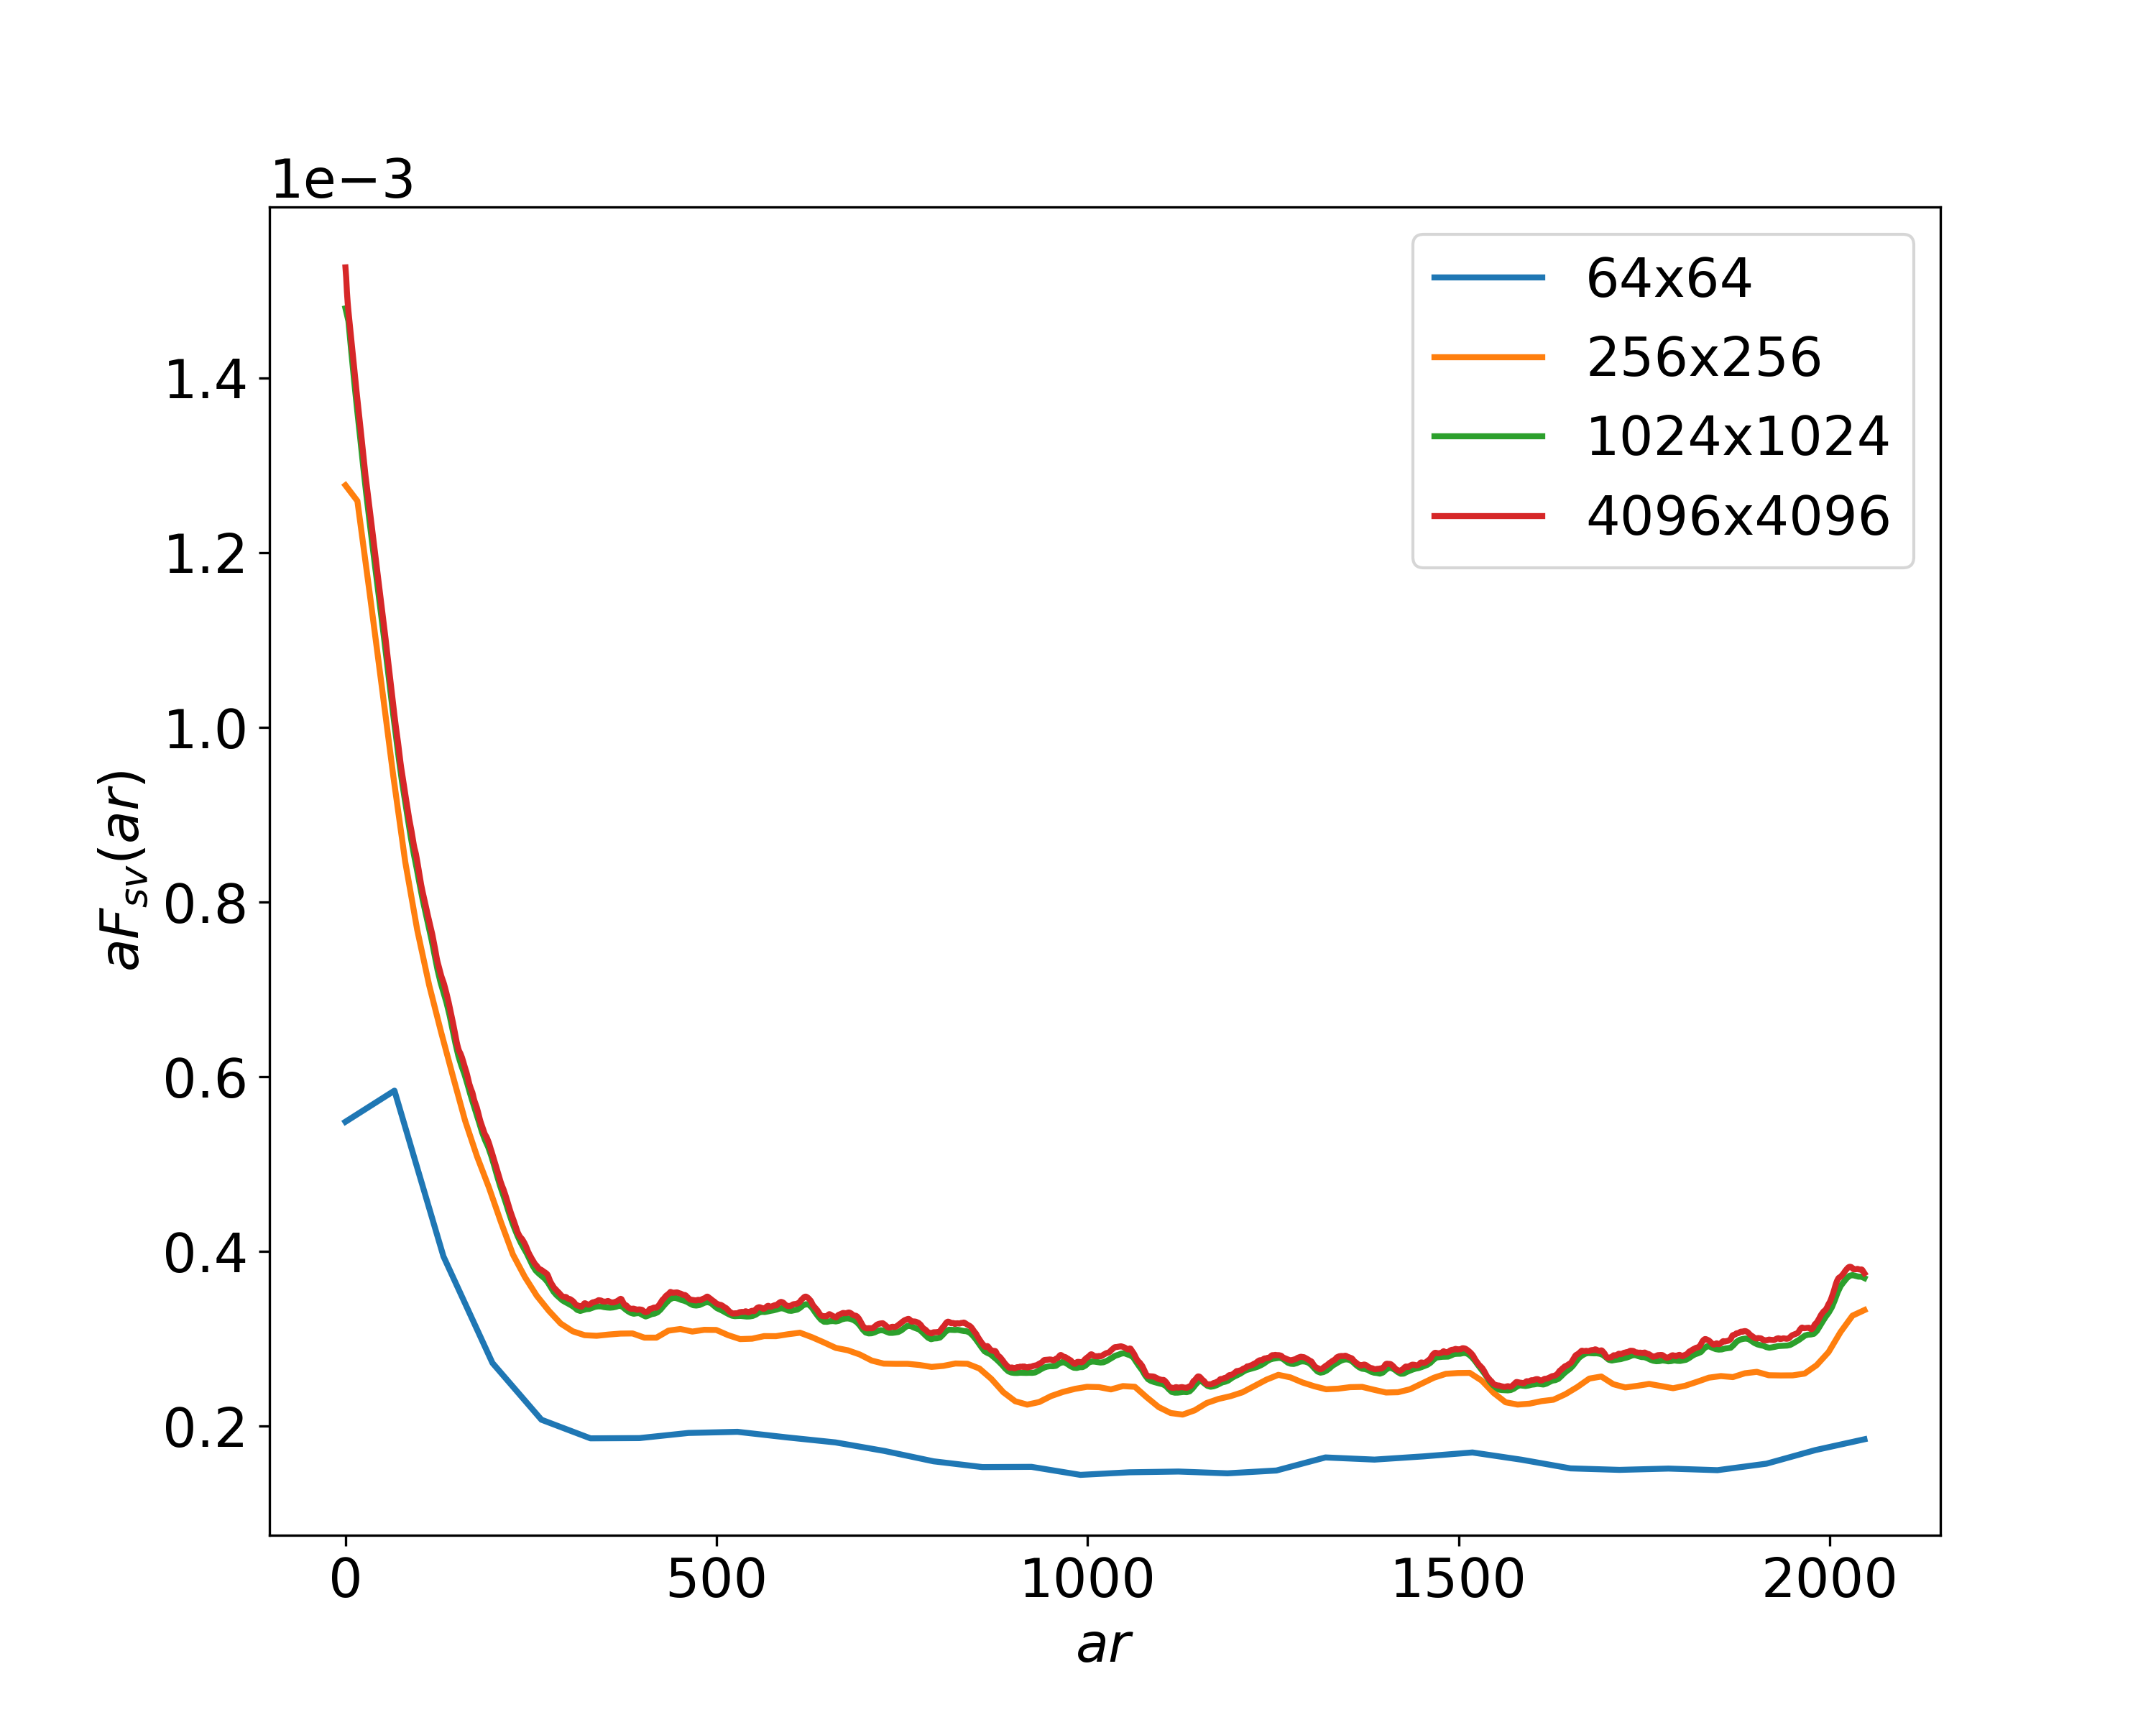
\includegraphics[width=0.475\linewidth]{images/plot-sv-noise.png}
    \label{fig:fsv-scaling-noise}}
  \caption[]{Surface-surface and surface-void correlation functions for
    images of overlapping disks and thresholded value noise obtained with
    different resolution. Theoretical results are also shown for overlapping
    disks.}
  \label{fig:scaling-alltogether}
\end{figure*}

We can observe two effects when downscaling the original image. The
first effect is that $F_{ss}(ar)$ and $F_{sv}(ar)$ for downscaled images lack in
detail (i.e. they are less ``noisy''). This can be easily explained by that the
interface between phases that becomes ``simpler'' when resolution decreases. The
second and much more important effect is that both correlation functions become
largely underestimated with the decline in resolution. This latter effect is in
general connected to the fact that the interface in digital images has
non-negligible thickness -- i.~e. the difference between real ``continuous''
interface versus ``digital'' interface (\cref{fig:scheme}). It is logical to
assume that with increasing spatial resolution the influence of this thickness
will diminish. This is exactly what we observe on \cref{fig:scaling-alltogether}
(\textcolor{red}{upper row}) where increasing disk discretization leads to
convergence with analytical solution; the accuracy of the computed CFs is almost
perfect for discretization of about 62 pixels for each disk's diameter. A
natural question arises: ``Is there a criterion of image quality (resolution)
that allows to predict the quality of surface CFs evaluation from digital
images?''. Turns out there is a possibility to establish such an empirical
criterion based on spectral analysis of input images and \cref{sec:crit} will
provide all necessary details.

\subsection{Convergence of correlation functions with increasing resolution}
\label{sec:value-noise}
Now consider a situation when an image is obtained by taking samples of a function
$f: \mathbb{R}^n \rightarrow \left\{0, 1\right\}$. The samples are taken from a
regulary spaced lattice which covers the range $[0, L]^n$  with interval
$\Delta$ between samples. The resulting image has then $L/\Delta + 1$ pixels in
each dimension. We will show empirically that for any sequence $\Delta_k$ so
that $\Delta_{k+1} < \Delta_k$ and $\Delta_k \rightarrow 0$ sequences
$F_{ss}^{\Delta_k}(r)$ and $F_{sv}^{\Delta_k}(r)$ computed for images with
lattice interval $\Delta_k$ converge to some limit functions $F_{ss}(r)$ and
$F_{sv}(r)$.

An example of $f$ is a thresholded value noise function. A value noise is a
procedurally generated noise which in one-dimensional case works as
follows. Firstly define a family of regulary spaced lattices $U_k$ with points
in coordinates $2^{-k}n,\ n \in \mathbb{Z}$. Each point of a lattice is assigned
a randomly taken value in the range $[0, 1]$. Then for each $U_k$ define a
function $g_k(x): \mathbb{R} \rightarrow \mathbb{R}$ which interpolates random
values in $U_k$ lineary. A value noise function is defined as follows:
\begin{align*}
  g(x; n) &= \frac{\sum\limits_{k=0}^{n-1} 2^{-k}g_k(x)}{\sum\limits_{k=0}^{n-1}
    2^{-k}} \\
  &= \frac{2^n}{2^{n+1}-2} \sum\limits_{k=0}^{n-1} 2^{-k}g_k(x)
\end{align*}
Here $n$ is a parameter called the number of octaves. A thesholded noise is then
\begin{align*}
  f(x; n) = \Theta(g(x; n) - 1/2)
\end{align*}
where $\Theta(x)$ is the Heaviside step function. A generalization for higher
dimensionality is constructed using the sample principle. An example of
thesholded value noise with three octaves is depicted on
\cref{fig:disks-noise} (\textcolor{red}{lower row}). Correlation functions
calculated for the noise with $n = 3$ at different resolutions are on
\cref{fig:scaling-alltogether}. If we calculate surface-surface and surface-void
correlation functions for these images and scale them as described above, we
again converge to some ``true'' correlation functions for continuous function
$f$.

\subsection{Effects of image magnification}
As we have just observed for analytical Poisson disks and arbitrary structures
based on thresholded value noise, with increasing resolution (or in other words
-- descreasing coarsedness) of the image, surface correlation functions converge
to "infinite resolution" values that can be seen as a target of CFs
computations. On the other hand, if the the image at hand is of limited
resolution, it would be very practical to know if rescaling this image with
increased resolution can lead to acceptable surface-surface functions
evaluation. To explore such a possibility we tried different methods to magnify
the image: bilinear, bicubic and nearest-neighbor interpolation.

To have true CFs for a comparison, we again utilize analytical Poisson disks: a
low-resolution and high-resolution images were produced by discretization of
disks at known positions, and then the low-resolution image was
magnified. Because the resized image becomes grayscale, we use the following
function as an indicator for the void phase provided the void phase is marked as
0 in the input image:
\begin{equation*}
  I^{(void)}(x) = (1 - x)^{1.5}.
\end{equation*}

We found that all interpolation methods are good for resizing purposes with
exception of nearest-neighbor approach. As an example, \cref{fig:resized} shows
the images of overlapping disks with almost the same surface-surface and
surface-void functions. The values of CFs are almost identical for
high-resolution and magnified images; the only flaw being the difference in
$F_{SS}$ for resized and digitized images due to pixelization of the interface
(the absence of "noise" on $F_{SS}$ for the rescaled image).

\begin{figure*}[ht]
  \centering
  \subfigure[The image resulting from digitizing of Poisson disks to
    the size of $300 \times 300$ pixels, and then magnified to
    $4000 \times 4000$ pixels using bilinear interpolation]{
    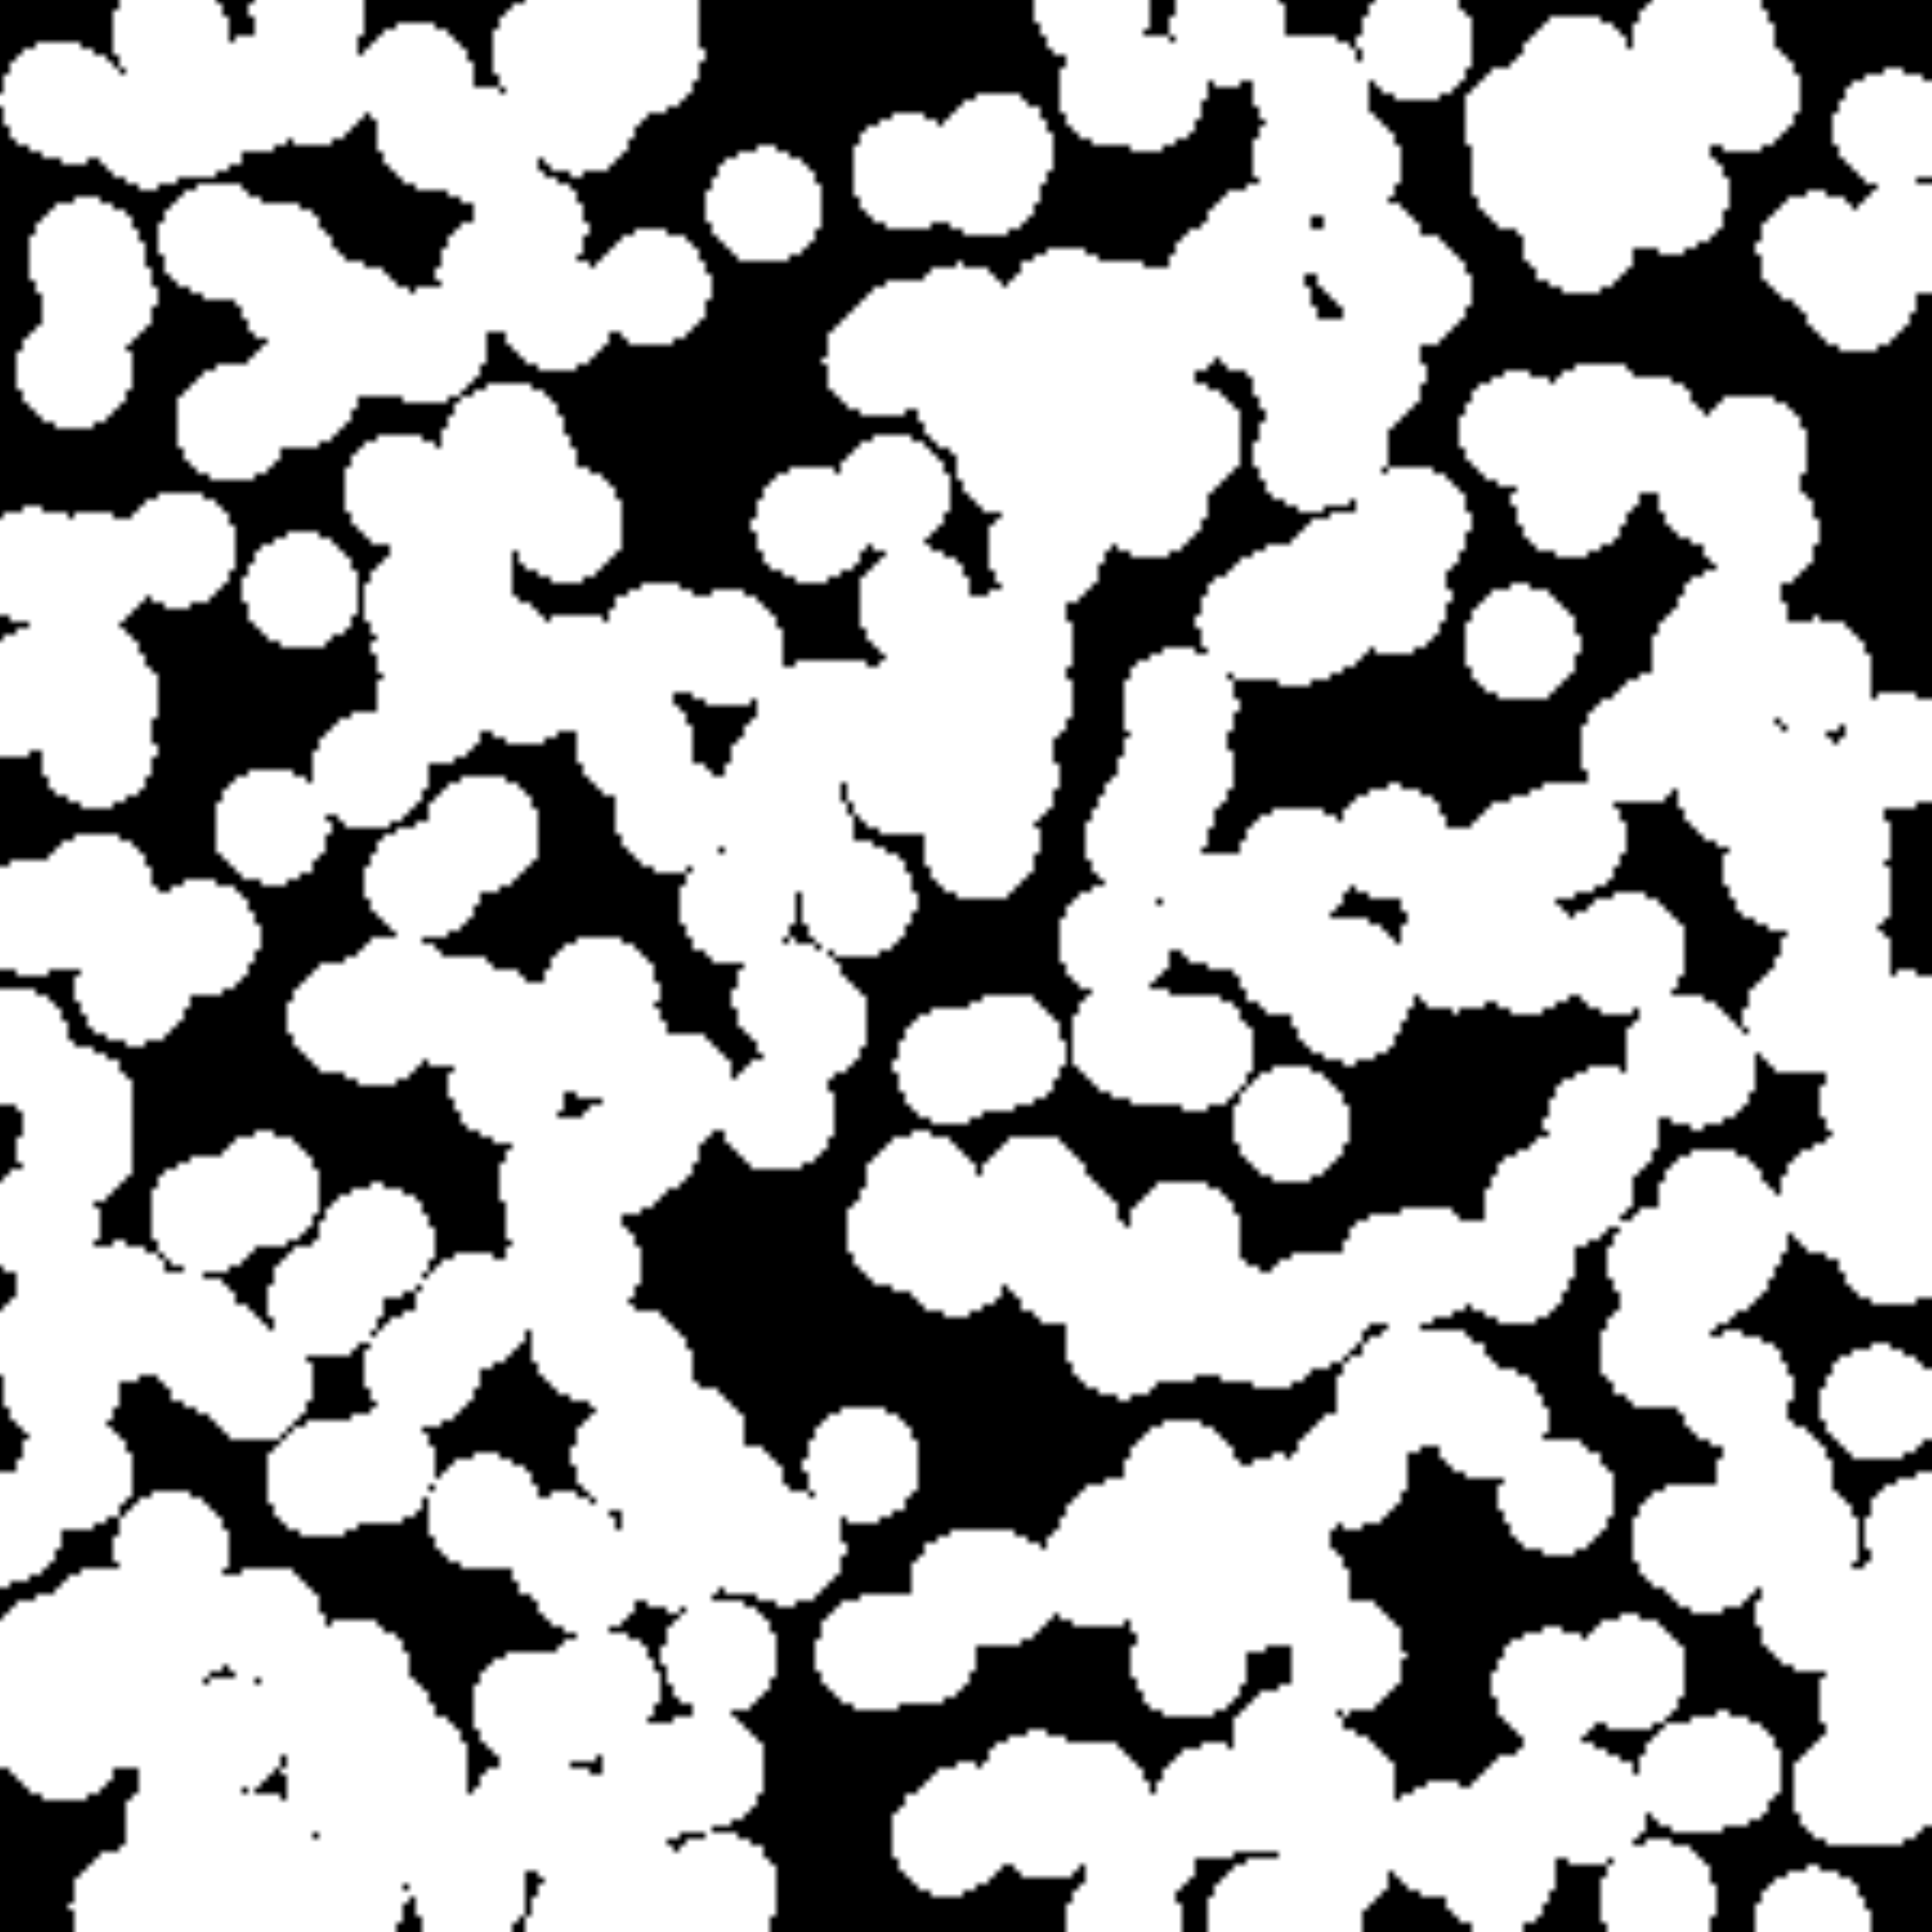
\includegraphics[width=0.25\linewidth, frame]{resize-effects/disks-bilinear.png}
    \label{fig:resized-bilinear}}
  \subfigure[Digitized image of Poisson disks with the size of
    $4000 \times 4000$ pixels]{
    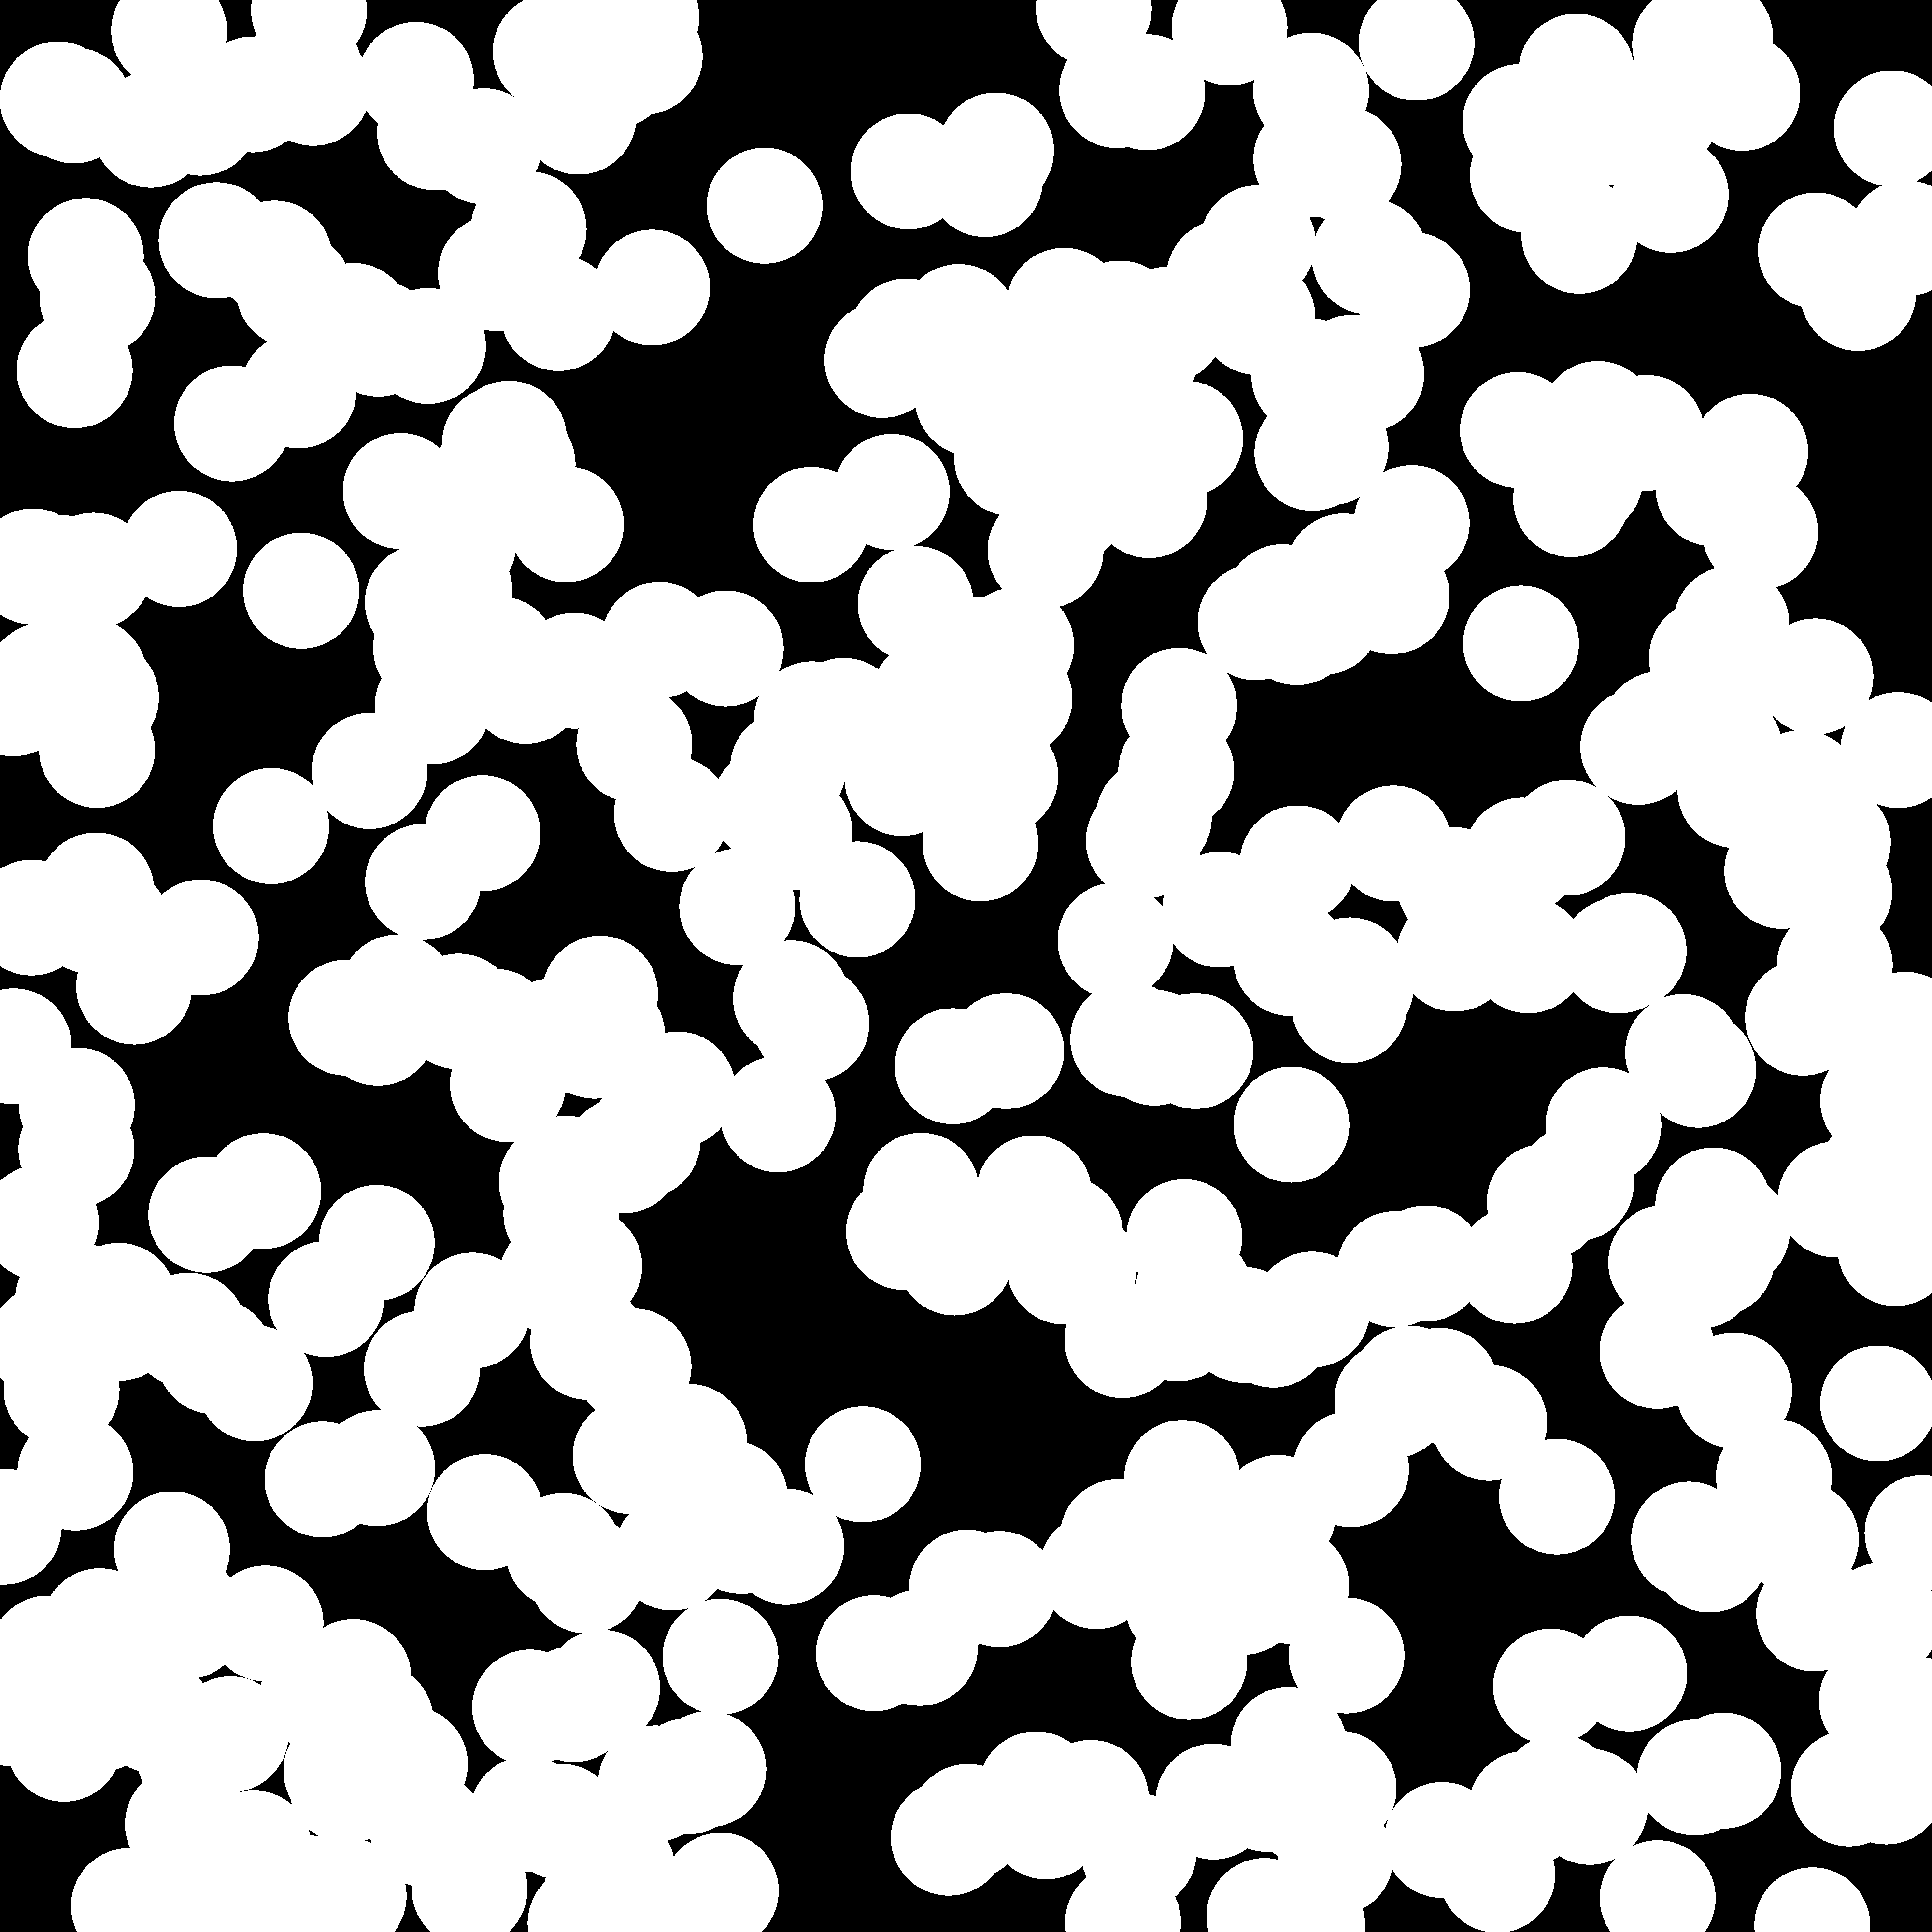
\includegraphics[width=0.25\linewidth, frame]{resize-effects/disks-big.png}
    \label{fig:resized-true}}
  \vskip\baselineskip
  \subfigure[Surface-surface functions]{
    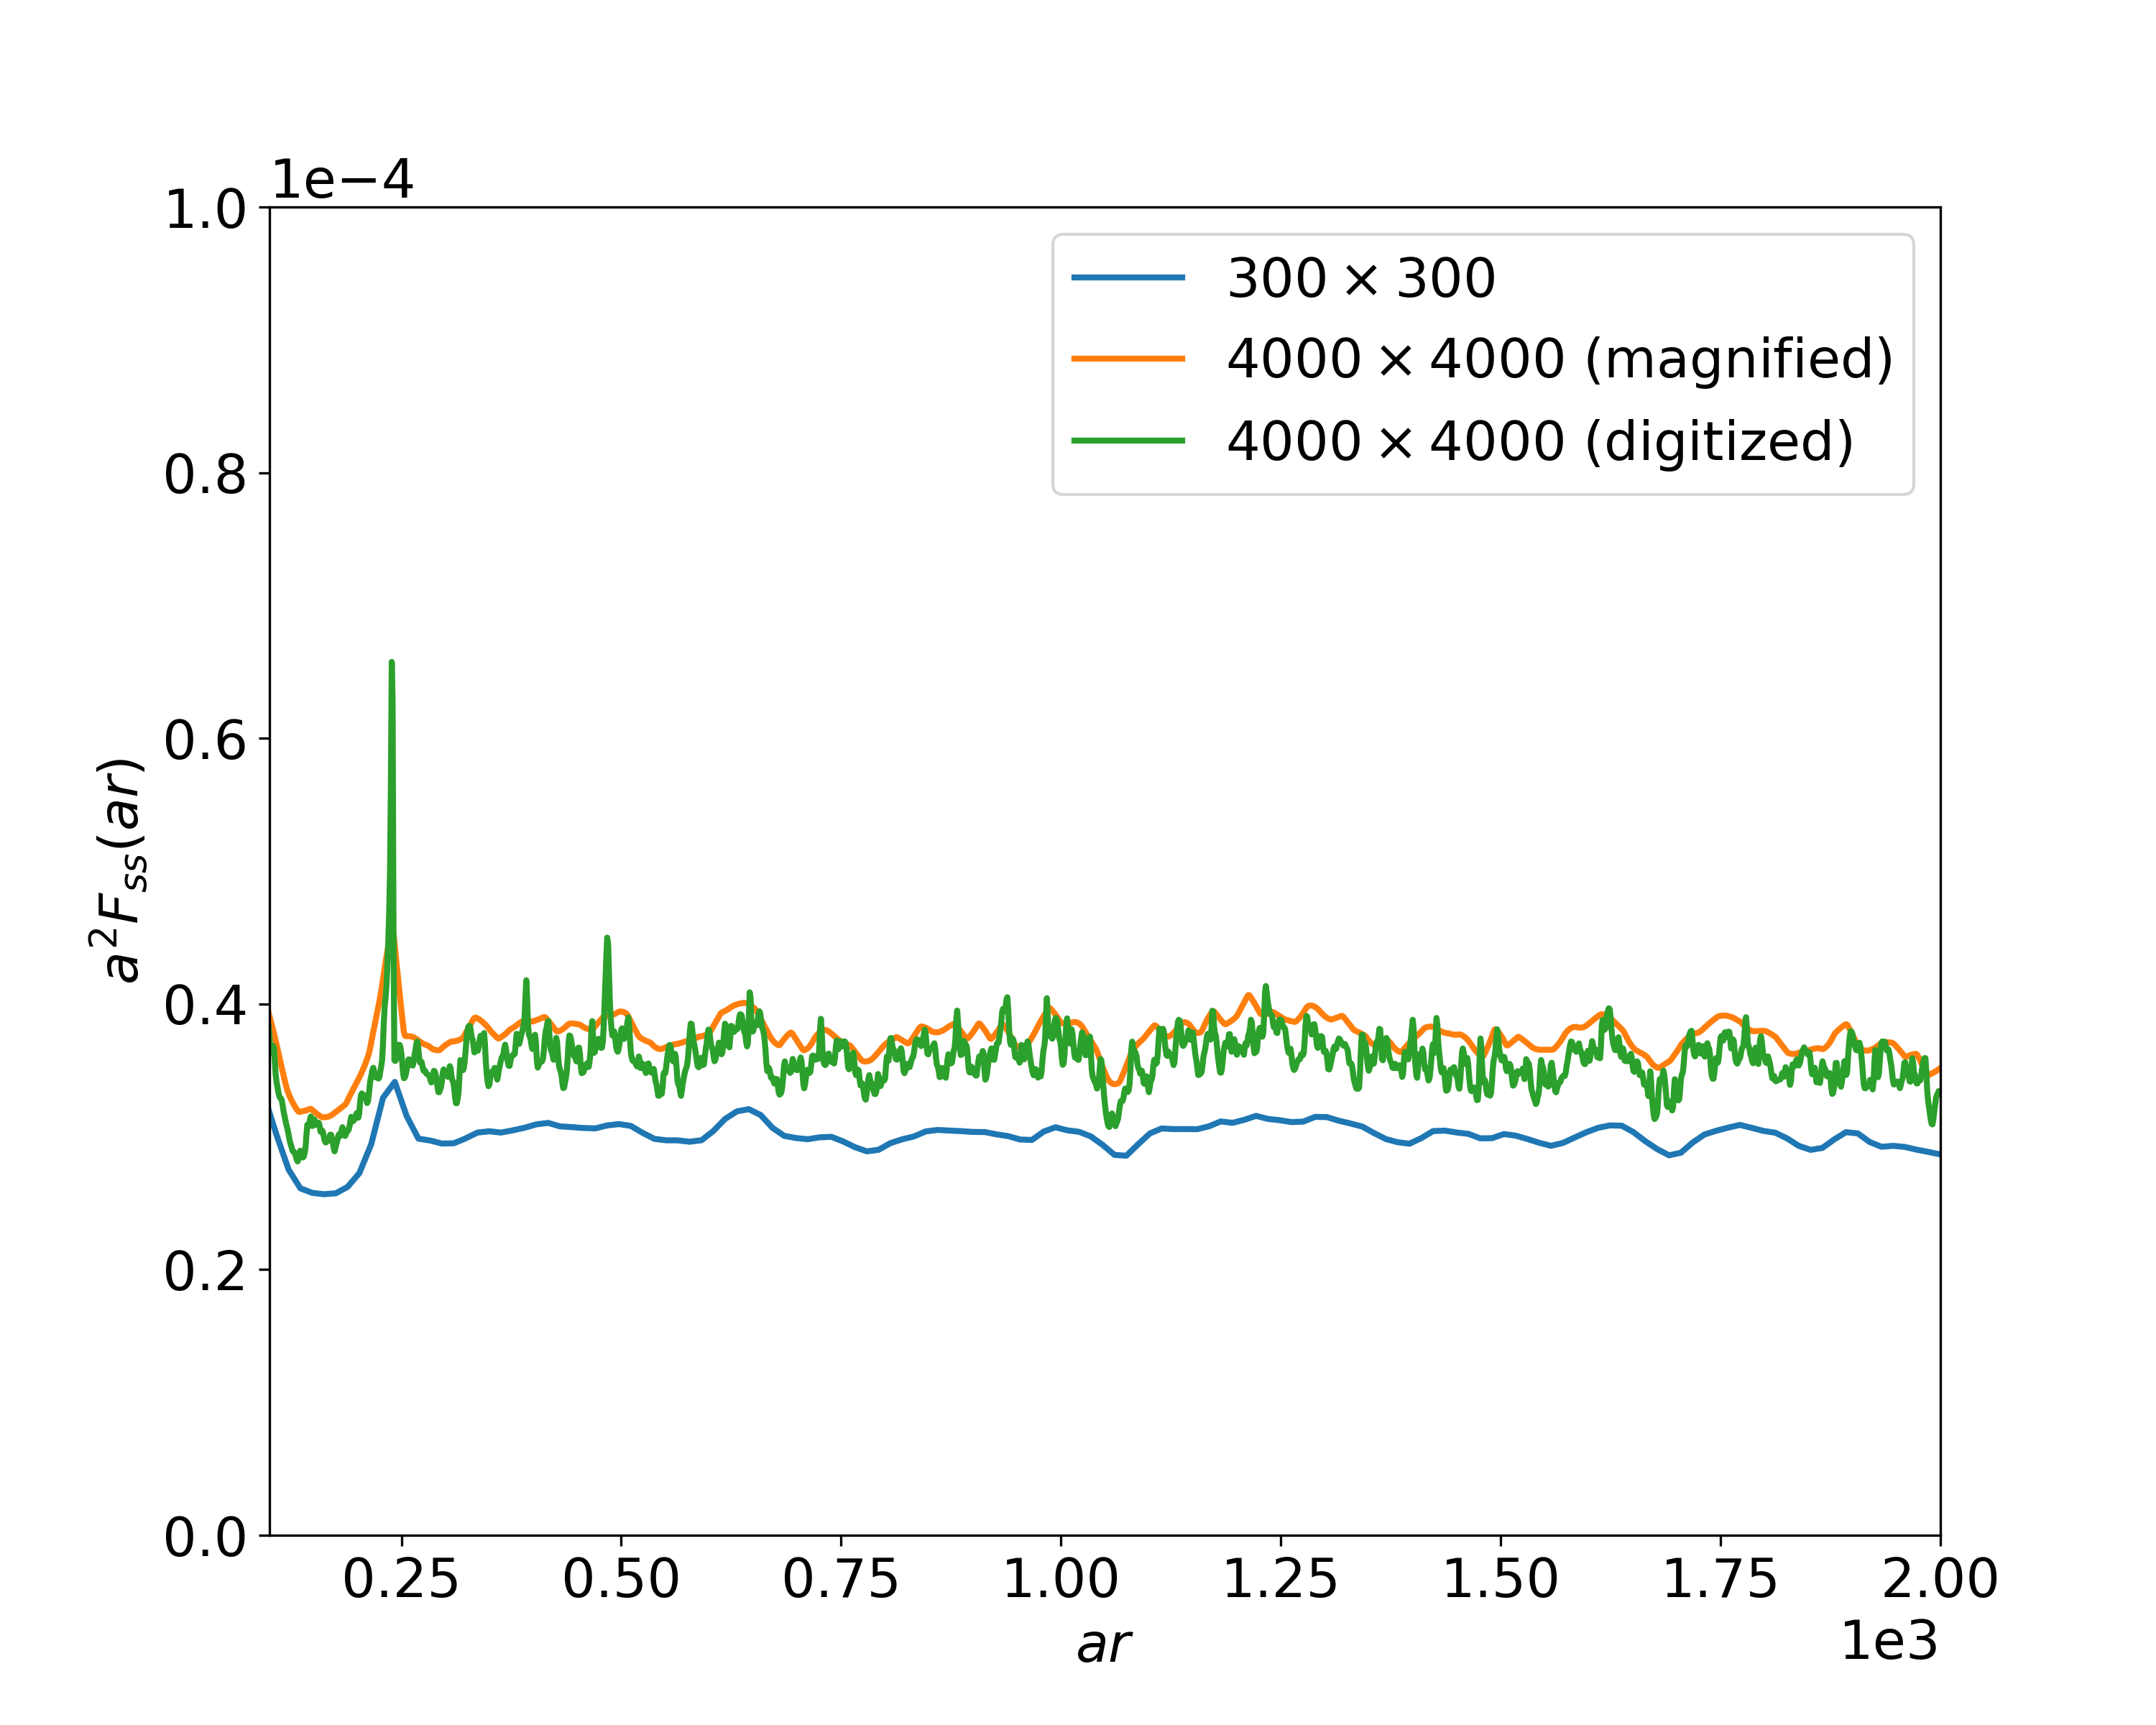
\includegraphics[width=0.45\linewidth]{resize-effects/surfsurf.png}
    \label{fig:resized-ss}}
  \hfill
  \subfigure[Surface-void functions]{
    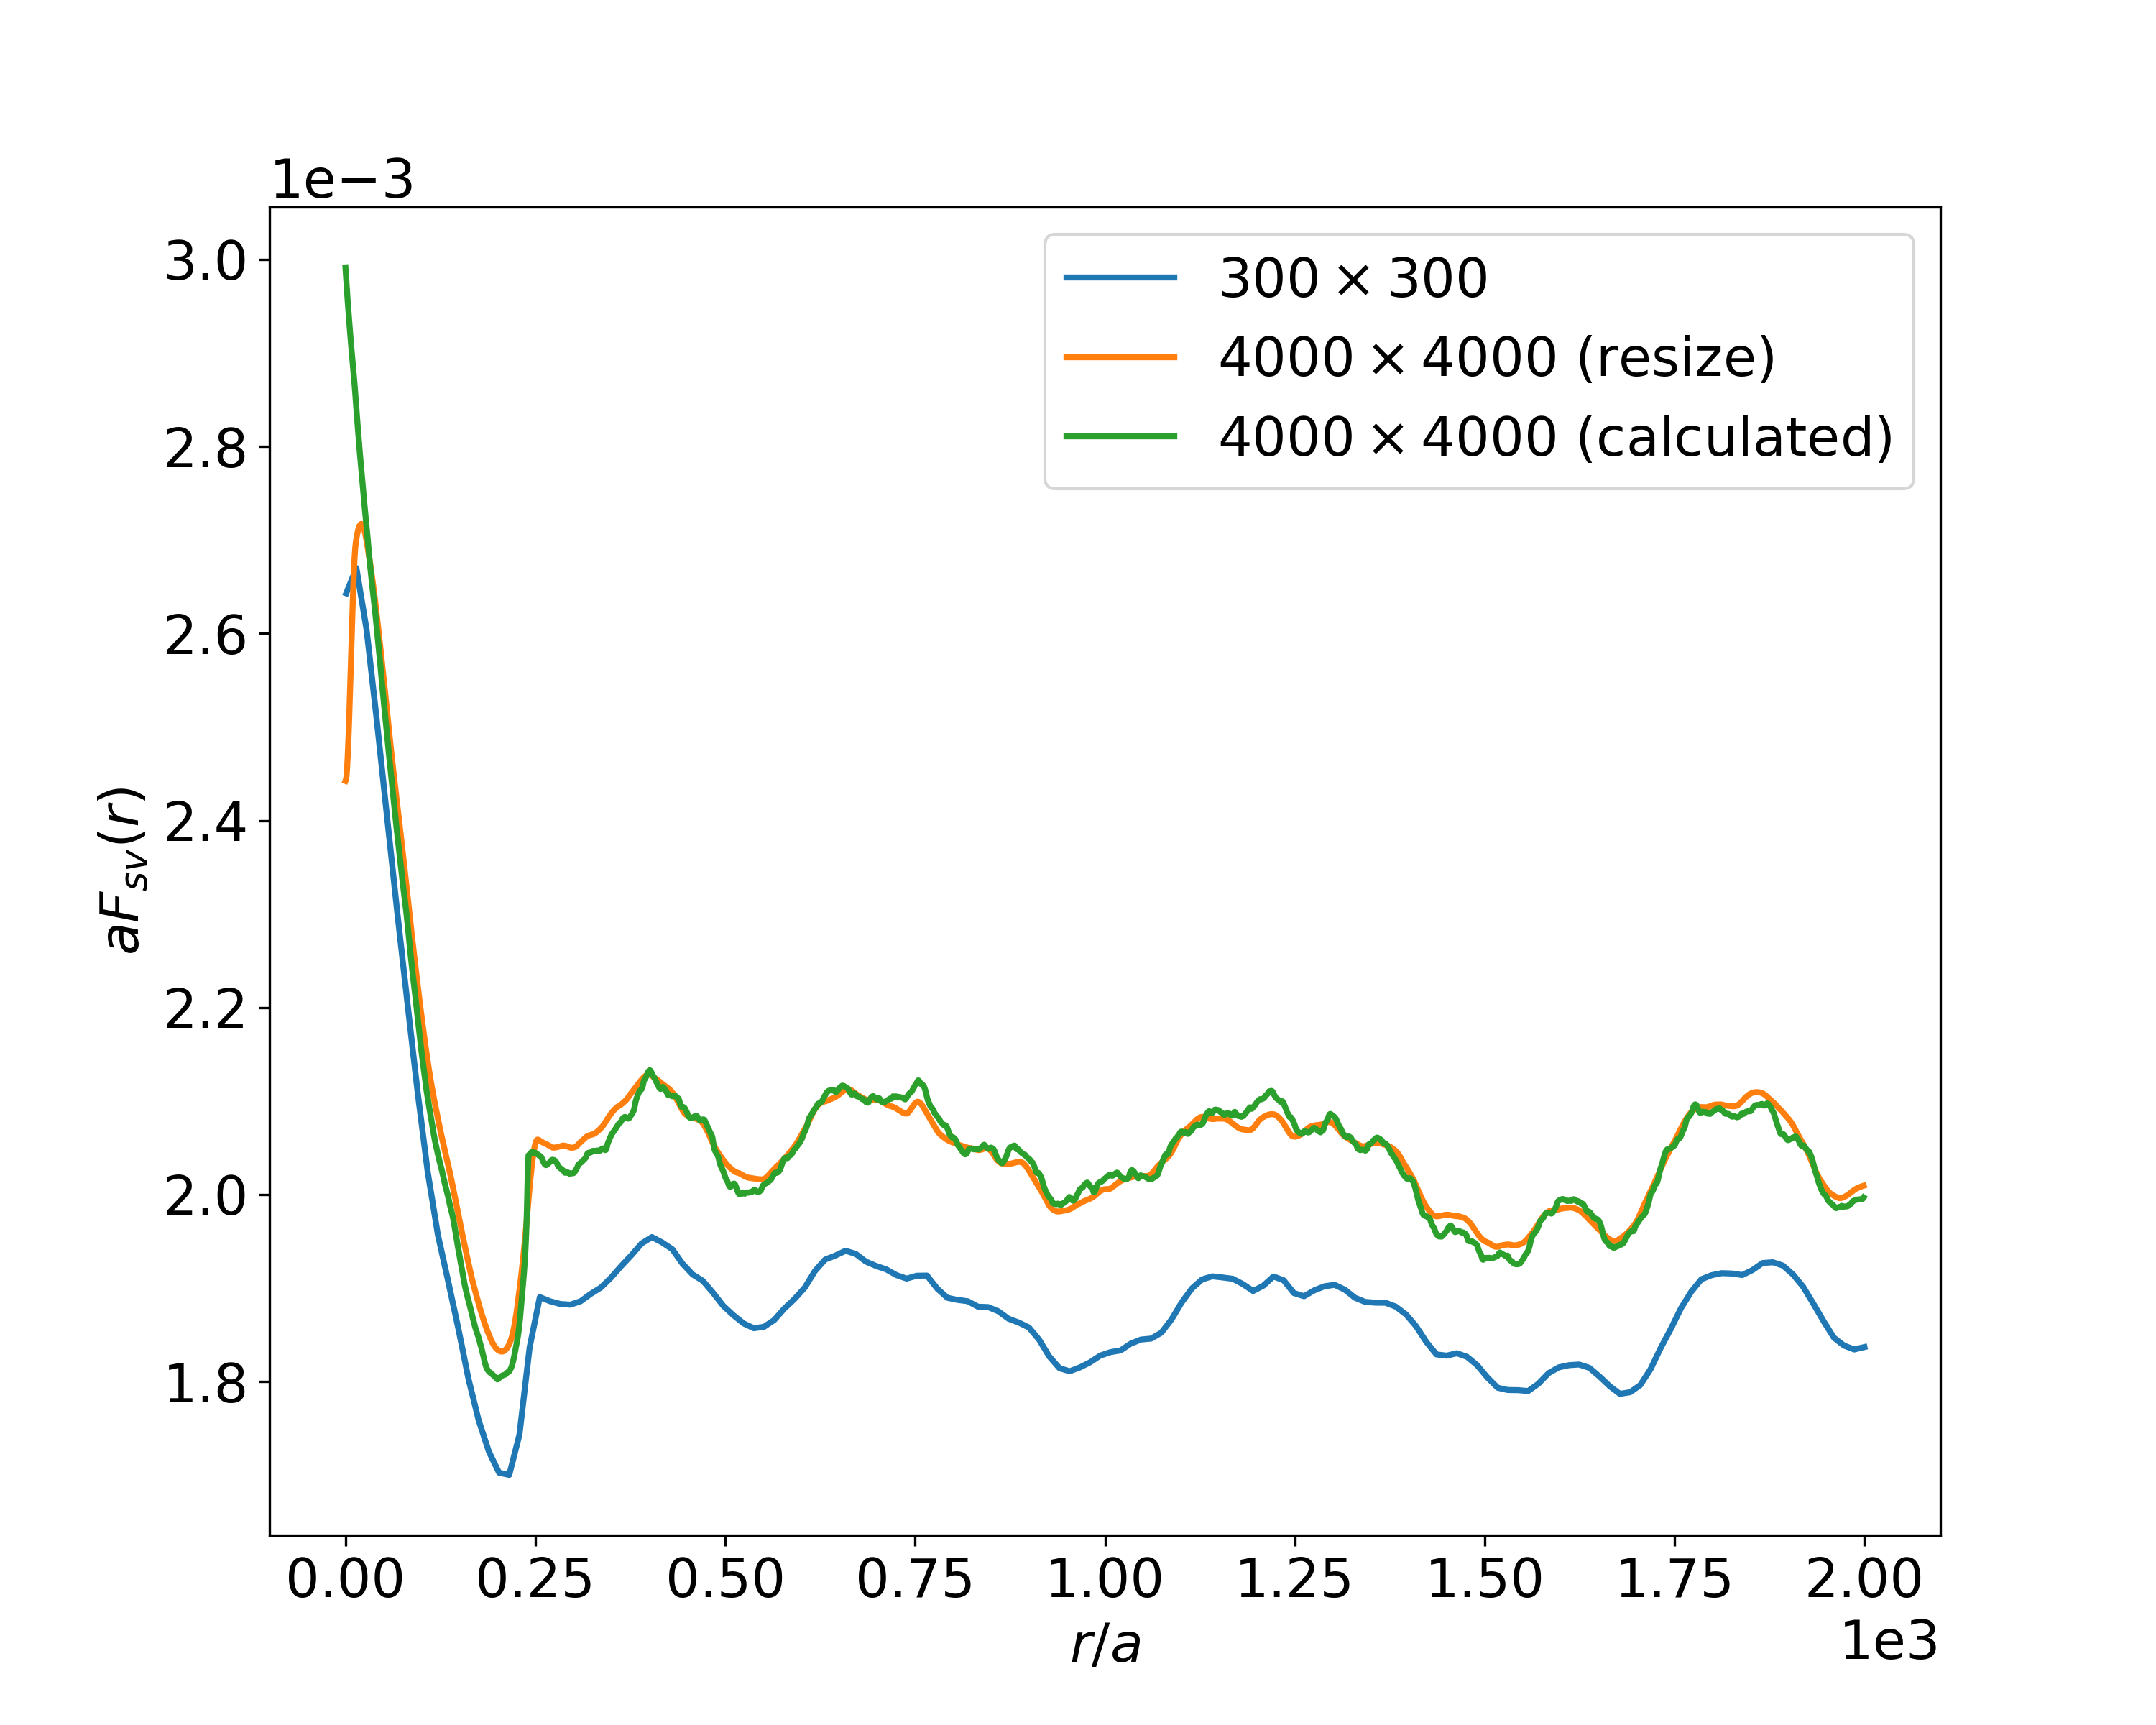
\includegraphics[width=0.45\linewidth]{resize-effects/surfvoid.png}
    \label{fig:resized-sv}}
  \caption[]{An example of images with almost identical correlation functions
    obtained using different methods: direct digitalization from known disk
    positions and magnification using bilinear interpolation.}
  \label{fig:resized}
\end{figure*}

\subsection{Criterion for accurate evaluation of surface CFs from discrete images}
\label{sec:crit}
Let us define one-dimensional forward ($F$) and inverse ($F^{-1}$) Fourier
transforms as:
\begin{align}
  \hat{f}(z) &= F[f](z) = \frac{1}{\sqrt{2\pi}}\int_{-\infty}^{\infty} f(x)
  e^{-i\pi xz} dx \label{eq:fourier-forward} \\
  f(x) &= F^{-1}[\hat{f}](z) = \frac{1}{\sqrt{2\pi}}\int_{-\infty}^{\infty} \hat{f}(z)
  e^{i\pi xz} dz \label{eq:fourier-backward}
\end{align}

Here $f(x)$ and $\hat{f}(z)$ can be thought of as representations of a signal in
the time domain and the frequency domain, respectively. Both equations
\cref{eq:fourier-forward} and \cref{eq:fourier-backward} preserve norm on $L_2$:
$(f, f) = (\hat{f}, \hat{f})$. It is said that Fourier transform preserves
``energy'' of the signal. According to Riemann-Lebesgue lemma \cite{HilbertSpaces}
energy of any signal ``concentrates'' around low frequencies. A measure of how
much energy concentrated in low frequencies (for some definition of low
frequencies) is a key to the understanding of the problem of correctness of our
method. The Shannon sampling theorem \cite{HilbertSpaces} states that it is
possible to reconstruct a band-limited signal $f(x)$ whose frequencies lie in
the range $[0, f]$ from a sequence of samples $\left\{f_n\right\}$ if the
sampling rate is no less than $2f$. We introduce a parameter $C_a$:
\begin{align*}
  f_0(x) &= f(x) - \langle f(x) \rangle \\
  C_a &= \frac{\int_{-a\omega}^{a\omega} |\hat{f_0}(z)|^2
    dz}{\int_{-\omega}^{\omega} |\hat{f_0}(z)|^2 dz}
\end{align*}
where $\omega = 2\pi f$ and $\langle f(x) \rangle$ is the mean value of $f(x)$
over its domain. The criterion for correctness is then:
\begin{equation*}
  C_a > 1 - \xi
\end{equation*}
for some $a$ and $\xi$. This criterion tells us exactly how much energy in
$f_0(x)$ is concentrated in a low frequency range $[0, af]$ compared to the
whole range $[0, f]$. Here we propose $a = 0.5$ and $\xi = 0.07$ as
a strict criterion which is based on results of
\cref{sec:comparison}. For overlapping disks we immediately observe that the
image with resolution $4096 \times 4096$ has surface CFs very close to
analytical solution (\cref{fig:fss-scaling} - \cref{fig:fsv-scaling}) and
perfectly satisfy our $C_{0.5}$ criterion. The other three downscaled images
fail to do so. The first two images of value noise (with
resolution $4096 \times 4096$ and $1024 \times 1024$) pass the criterion and the
other two do not, which is in agreement with \cref{fig:fss-scaling-noise} -
\cref{fig:fsv-scaling-noise} (correlation functions converge at resolution about
$1024 \times 1024$).

Thus, we conclude after inspecting \cref{fig:disks-noise} and
\cref{fig:scaling-alltogether} that the criterion correctly selects images which
are suitable for calculation of surface correlation functions. The criterion
$C_{0.5}$ decays fast with a decline in the image resolution as demostrated in
\cref{fig:crit-plot}.

\begin{figure}[ht]
  \centering
  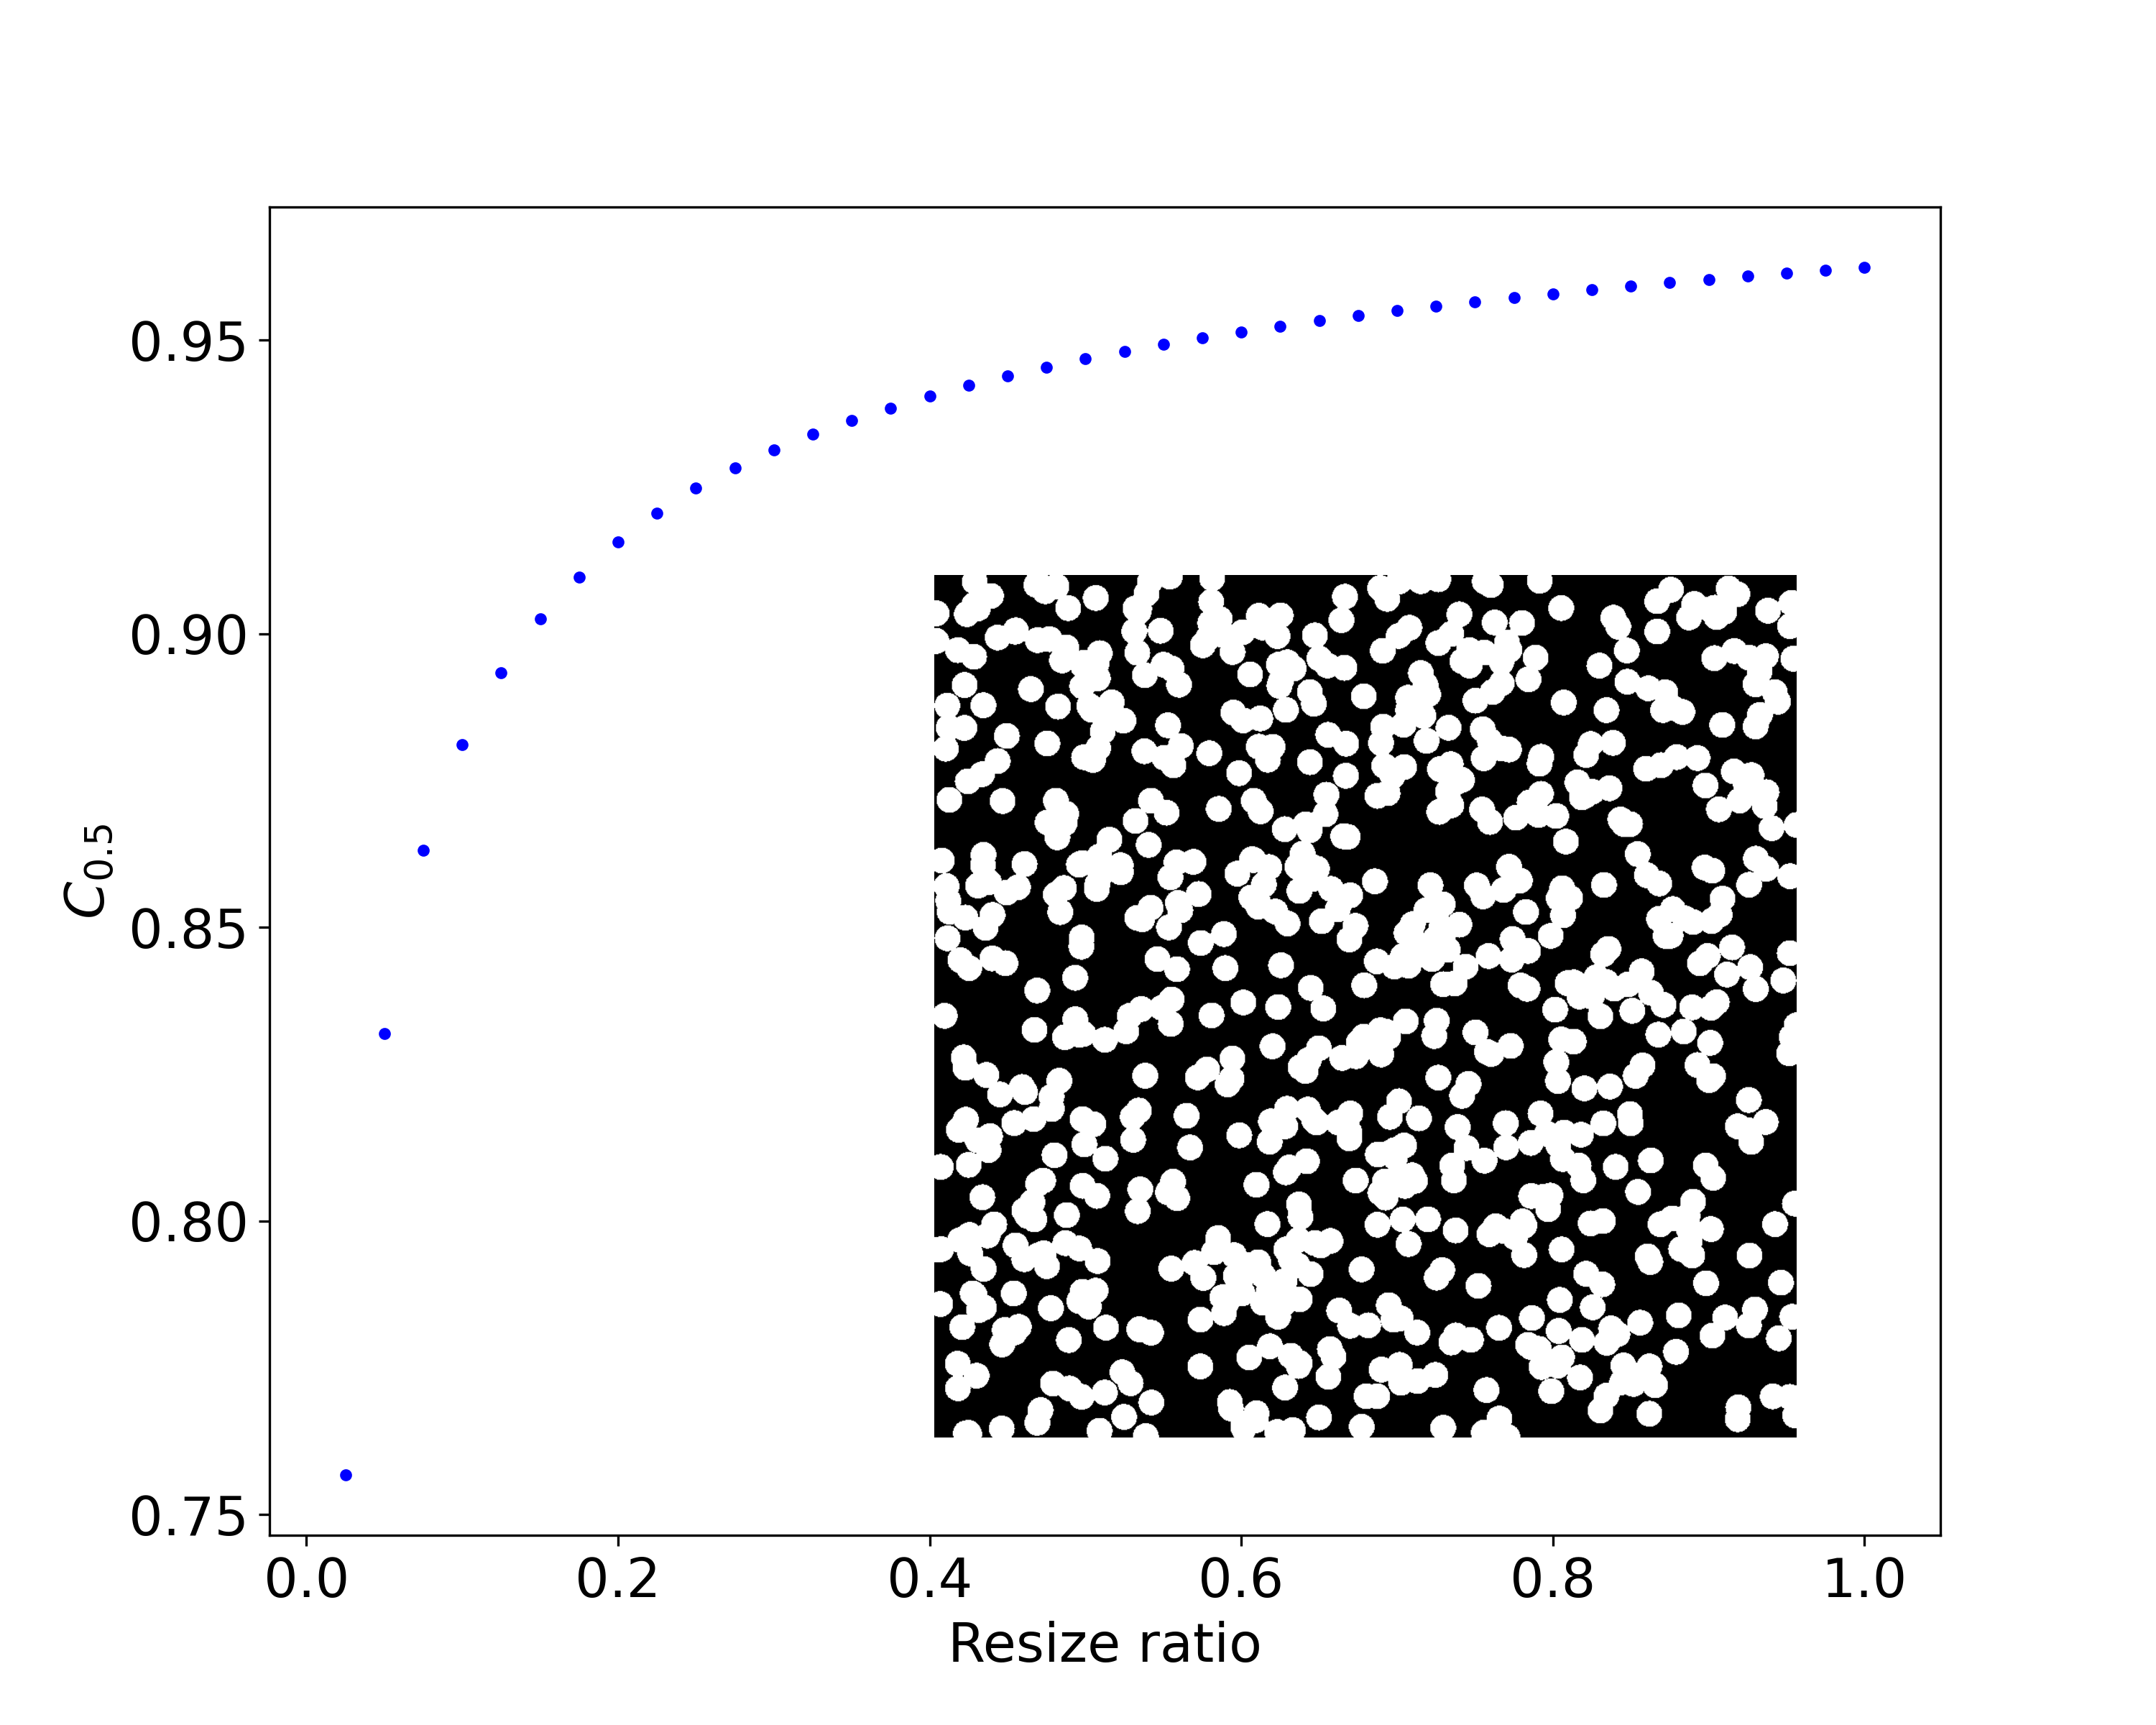
\includegraphics[width=\linewidth]{images/plot-criterion1.png}
  \caption[]{Decay of criterion $C_{0.5}$ as a function of the image resolution
    for the downscaled image (shown as a resize ratio). Original image is
    attached to the plot.}
  \label{fig:crit-plot}
\end{figure}

\subsection{The choice of method to extract the interface}
\begin{figure}[ht]
  \centering
  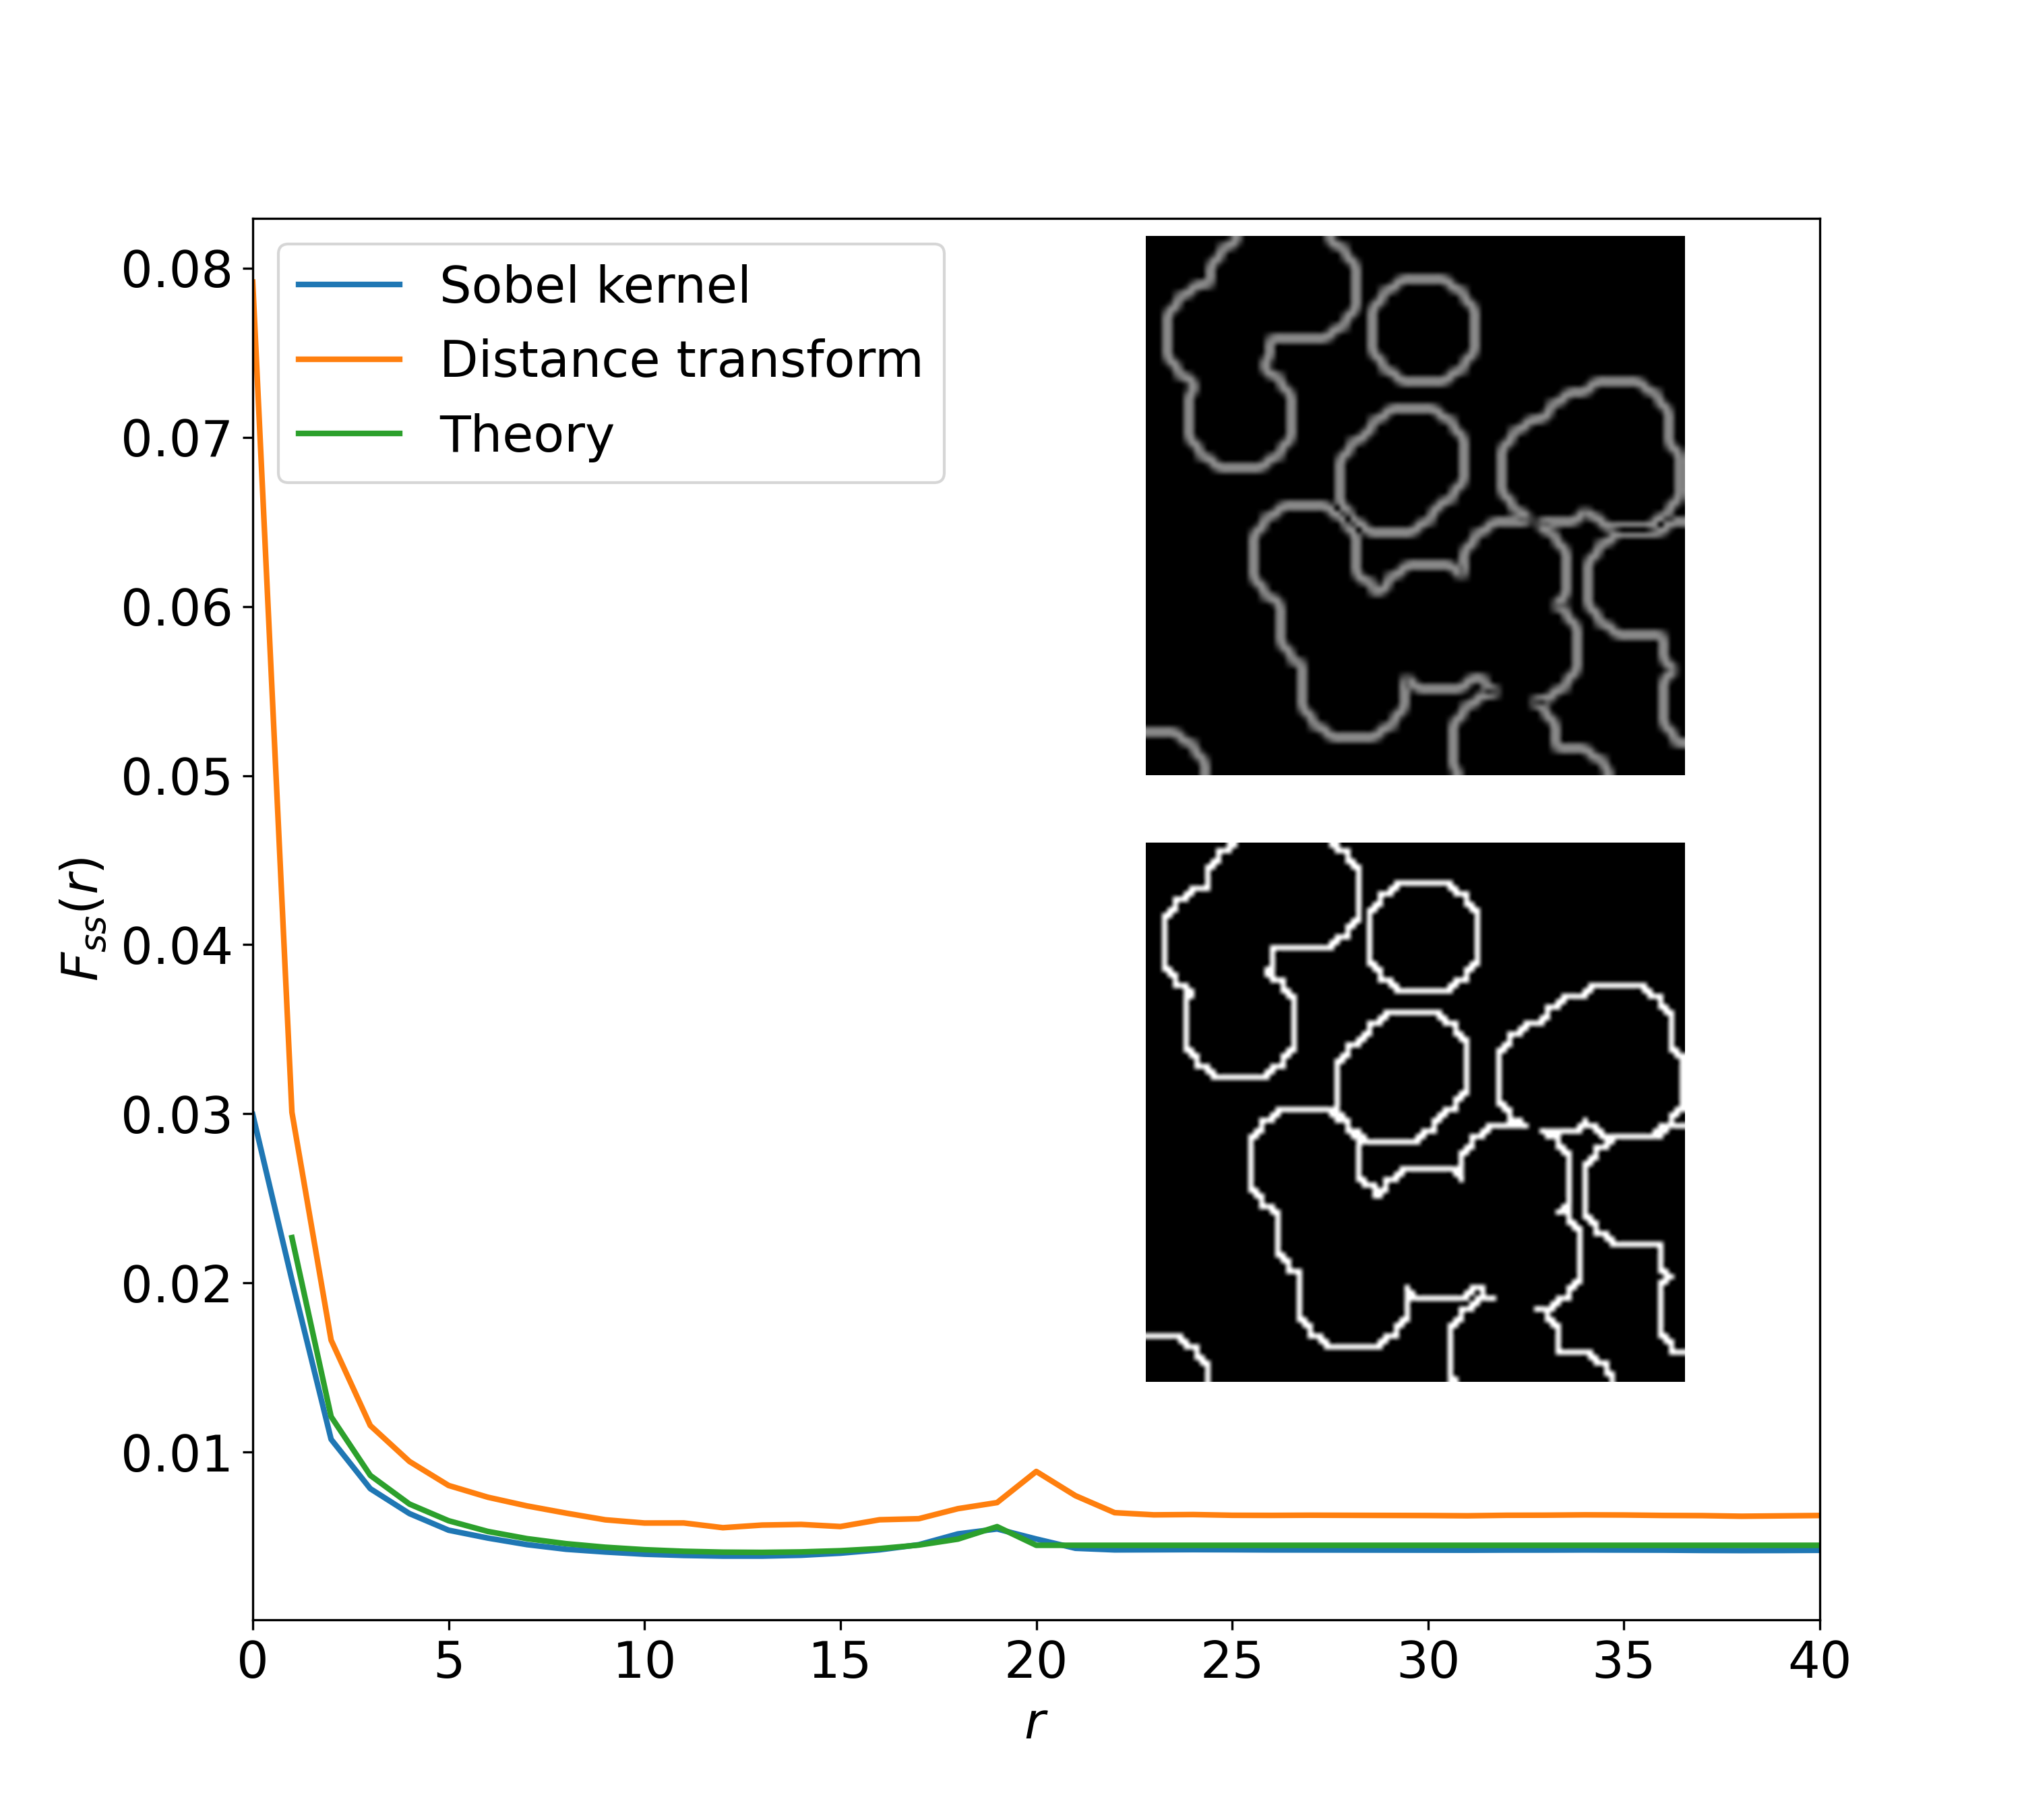
\includegraphics[width=\linewidth]{images/dm_sobel.png}
  \caption{Surface-surface correlation function calculated with different
    interface extraction methods (Sobel to the left, and distance map to the
    right on the insets). Discretization of each disk is 20 pixels per diameter,
    the size is $1000 \times 1000$ pixels.}
  \label{fig:interface-extraction}
\end{figure}

Finally, we explore all major edge-detecting filters, including "naive" distance
map approach. Surface-surface functions for overlapping Poisson disks
($R = 10,\ \lambda = 2 \cdot 10^{-3}$ on image with dimensions of $1000 \times 1000$
pixels) computed with different methods of interface extraction are shown on
\cref{fig:interface-extraction}. These methods include image filtering with
Sobel operator and interface extraction with distance map. When using distance
map both outer (\cref{eq:dist-outer}) and inner (\cref{eq:dist-inner})
interfaces are used to compute the correlation function. An average over the
last two functions is also shown. Sobel kernel clearly outperforms the distance
map approach. However, the result on \cref{fig:interface-extraction} could be
related to the resolution of studied image. If we now increase the disretization
of the disks and, thus, the image resolution
($R = 70,\ \lambda = 3 \cdot 10^{-6}$ on image with dimensions of
$5000 \times 5000$ pixels) we get the result as presented on
\cref{fig:sobel-vs-distance-map}. In this case the image filtering method again
collapses to an analytical solution whilst the distance map method failed to do
so. This subsection's results clearly advocate in favour of the edge-detection
filter in case of surface CFs evalution based on digital images.

To demostrate the possibilities to compute directional surface correlation
functions, on \cref{fig:direction-vs-map} we show a comparison of the ensemble
$F_{SS}$ computed by averaging the full correlation map against the CF computed
along a single direction (the input image is isotropic Poisson disks from
\cref{fig:interface-extraction}). As expected, less sampling results in more
noise but in general conincide with analytical and ensemble average computed
CFs.

\begin{figure}[ht]
  \centering
  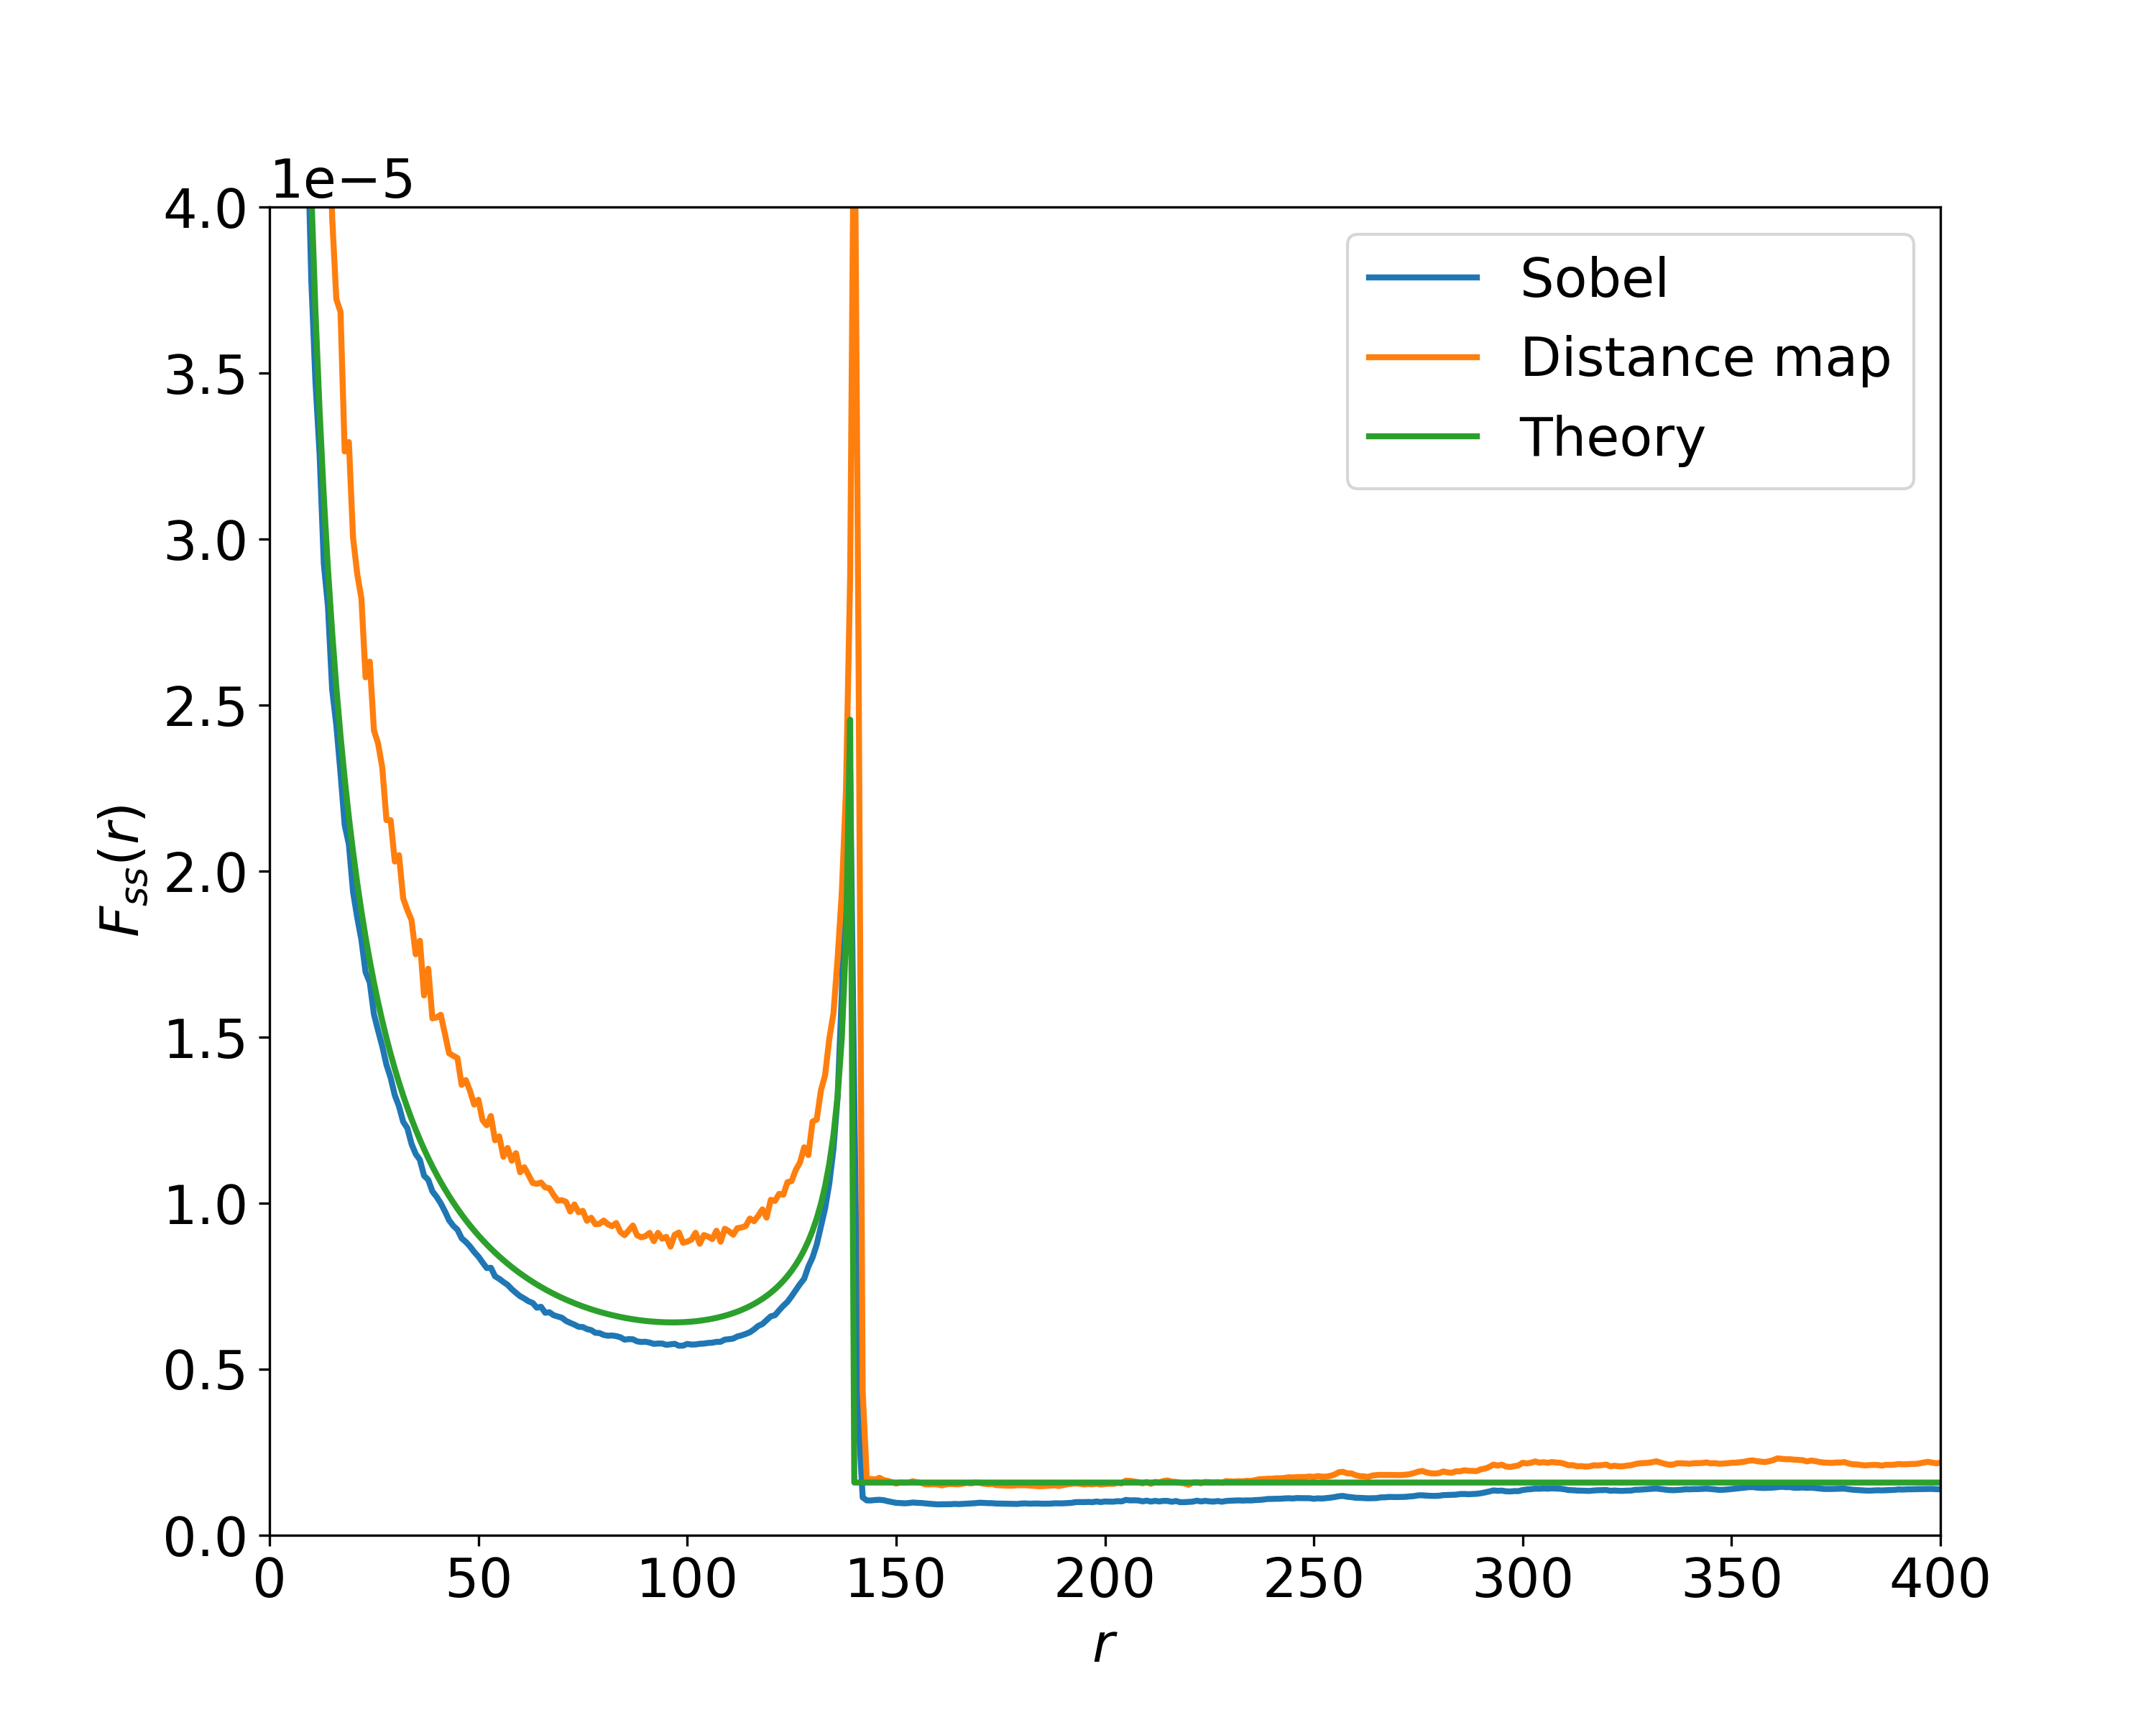
\includegraphics[width=\linewidth]{images/sobel-vs-distance-map.png}
  \caption{Comparison of Sobel filter and distance map approaches on
    high-resolution image with 140 pixels per disk diameter, the size is
    $5000 \times 5000$ pixels. \textcolor{red}{Please, put in the inset image}}
  \label{fig:sobel-vs-distance-map}
\end{figure}

\begin{figure}[ht]
  \centering
  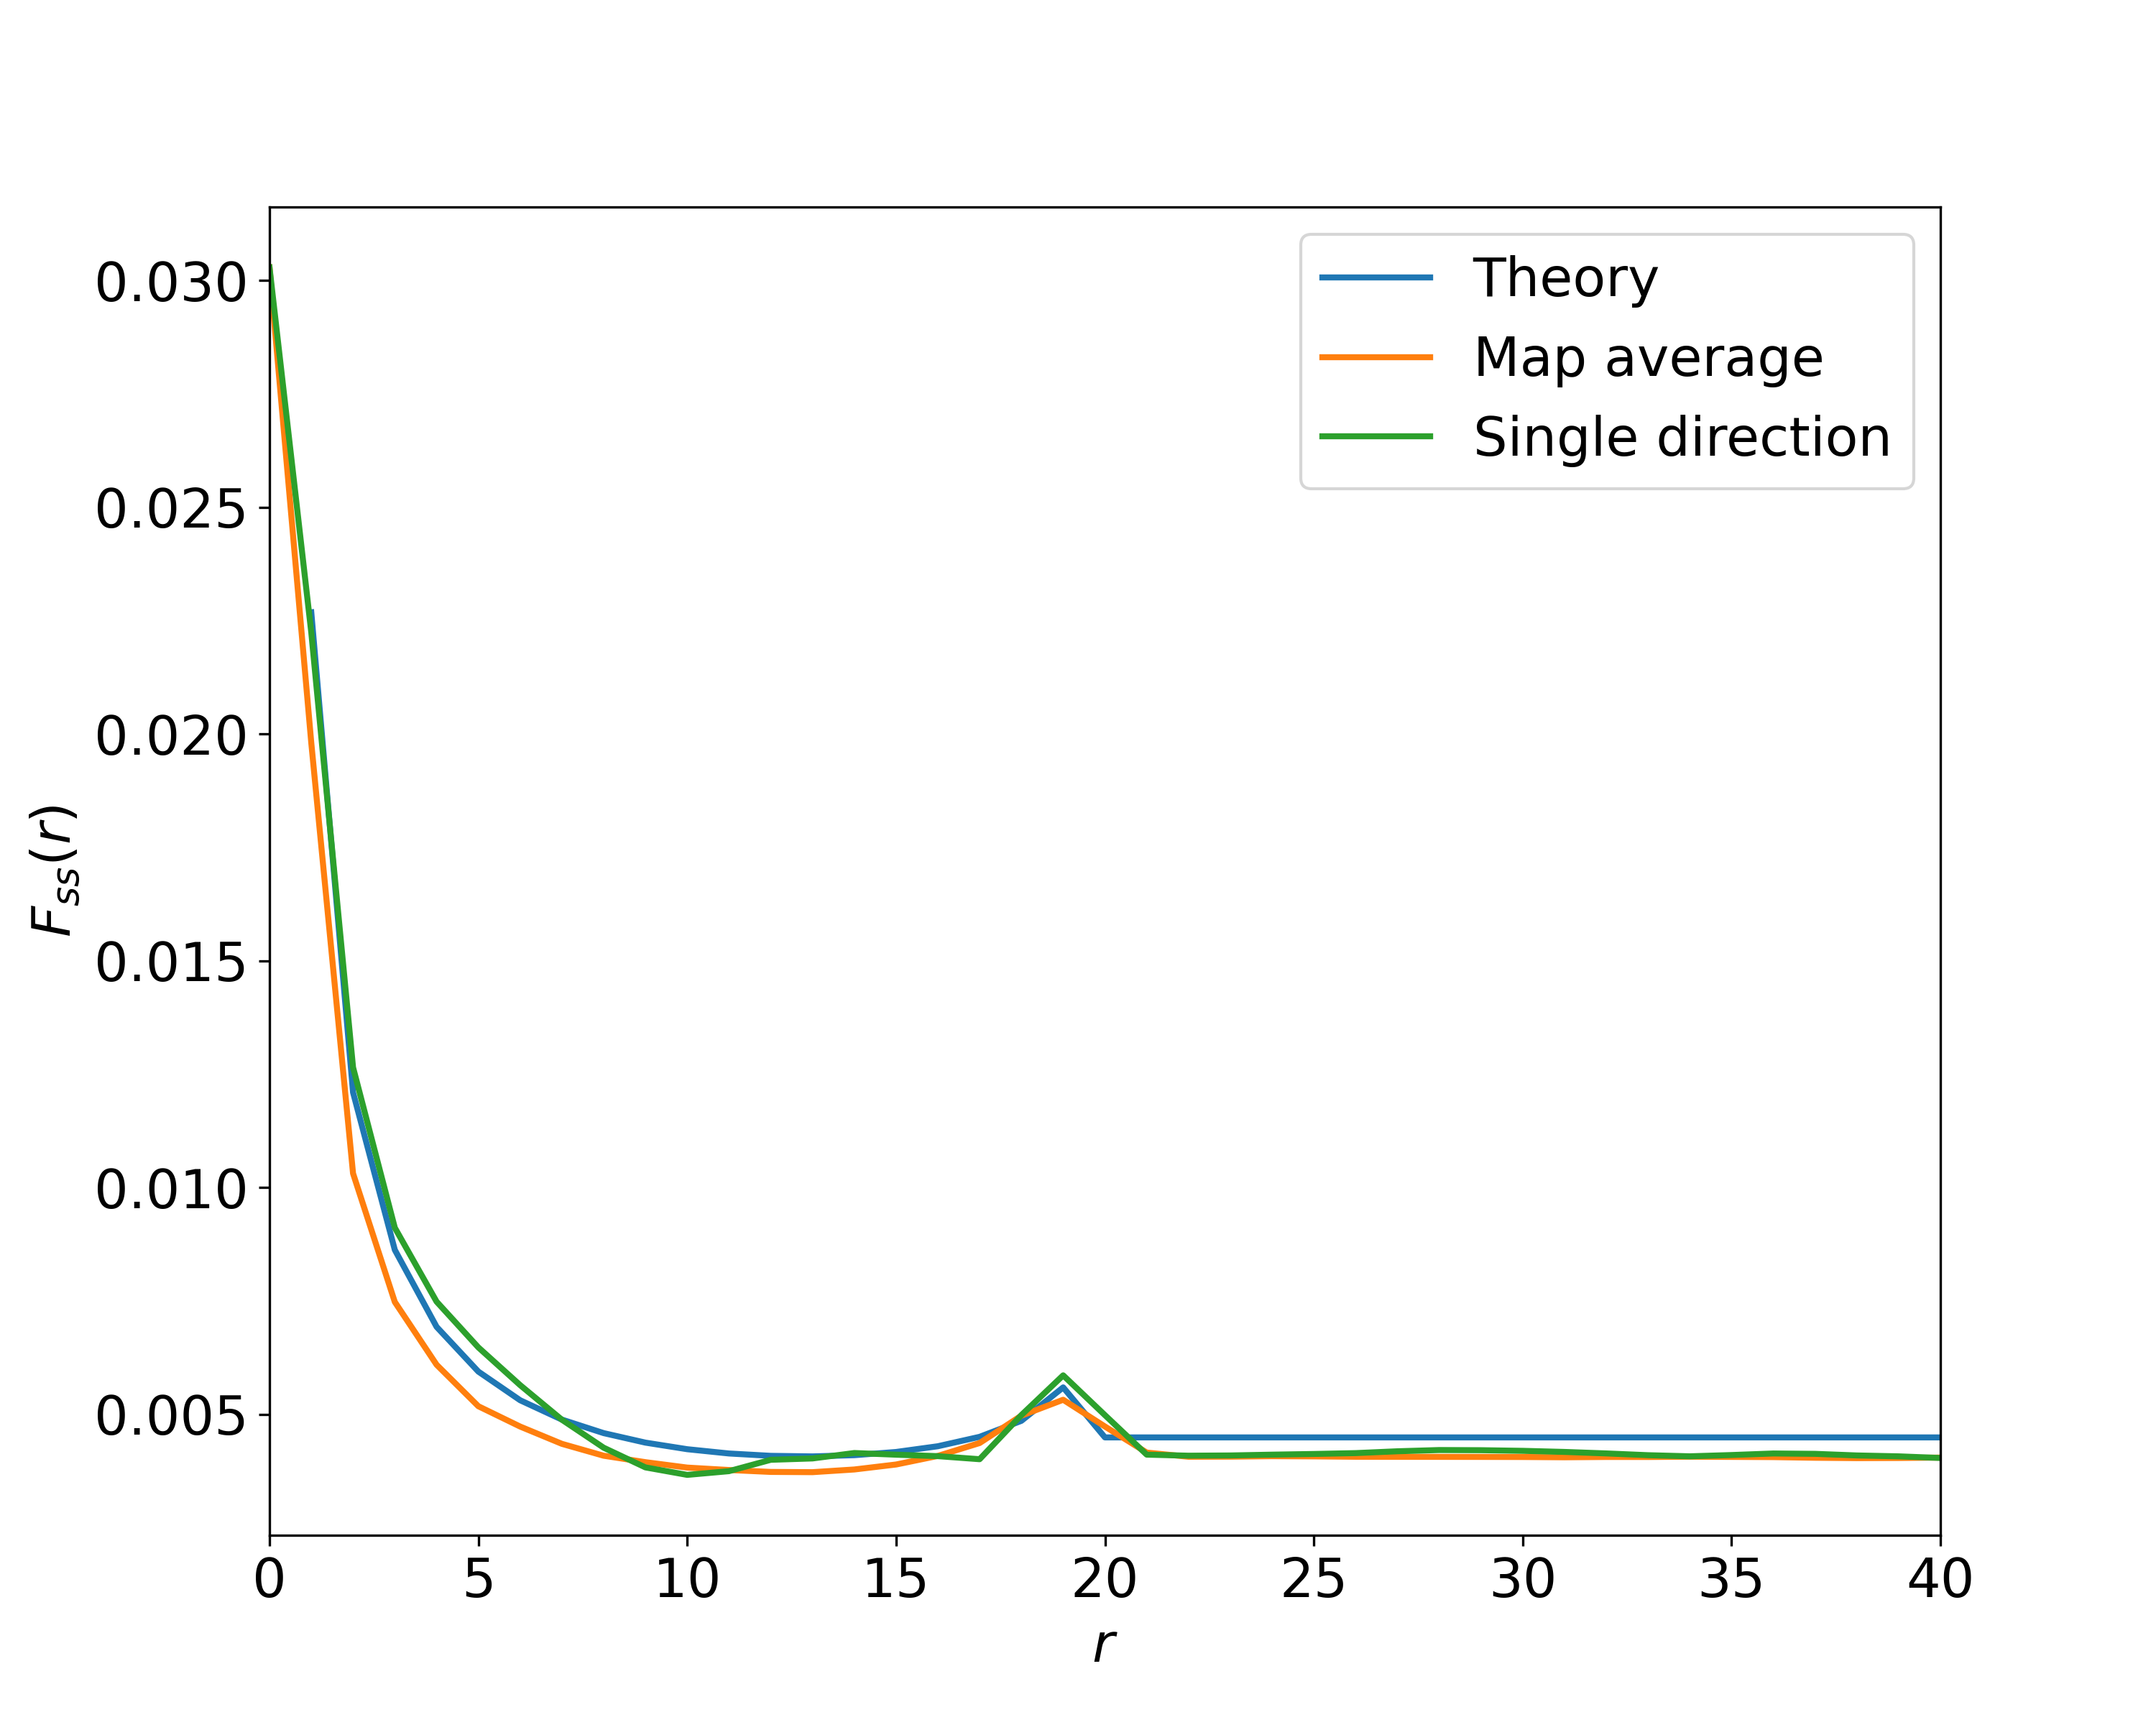
\includegraphics[width=\linewidth]{images/direction_and_map.png}
  \caption{The comparison of directional and ensemble averaged over the full map
    $F_{SS}$ \textcolor{red}{Please, put in the inset image}.}
  \label{fig:direction-vs-map}
\end{figure}

In addition to Sobel, there are plenty of other kernels for gradient evaluation
\cite{bickley1948,prewitt1970,ando2000}. In total, we investigated Sobel, Ando,
Sharr, Bickley and Prewitt filters. Their performance is almost the same
(\cref{fig:kernels}). The errors against the analytical solution are very
similar and the overall performance depends on the particular image. Therefore,
it is difficult to recommend specific kernel; so, the choice of the Sobel kernel
is purely due to the fact that this filter is a classical edge-detecting kernel
implemented in libraries for all major programming languages.

\begin{figure}[ht]
  \centering 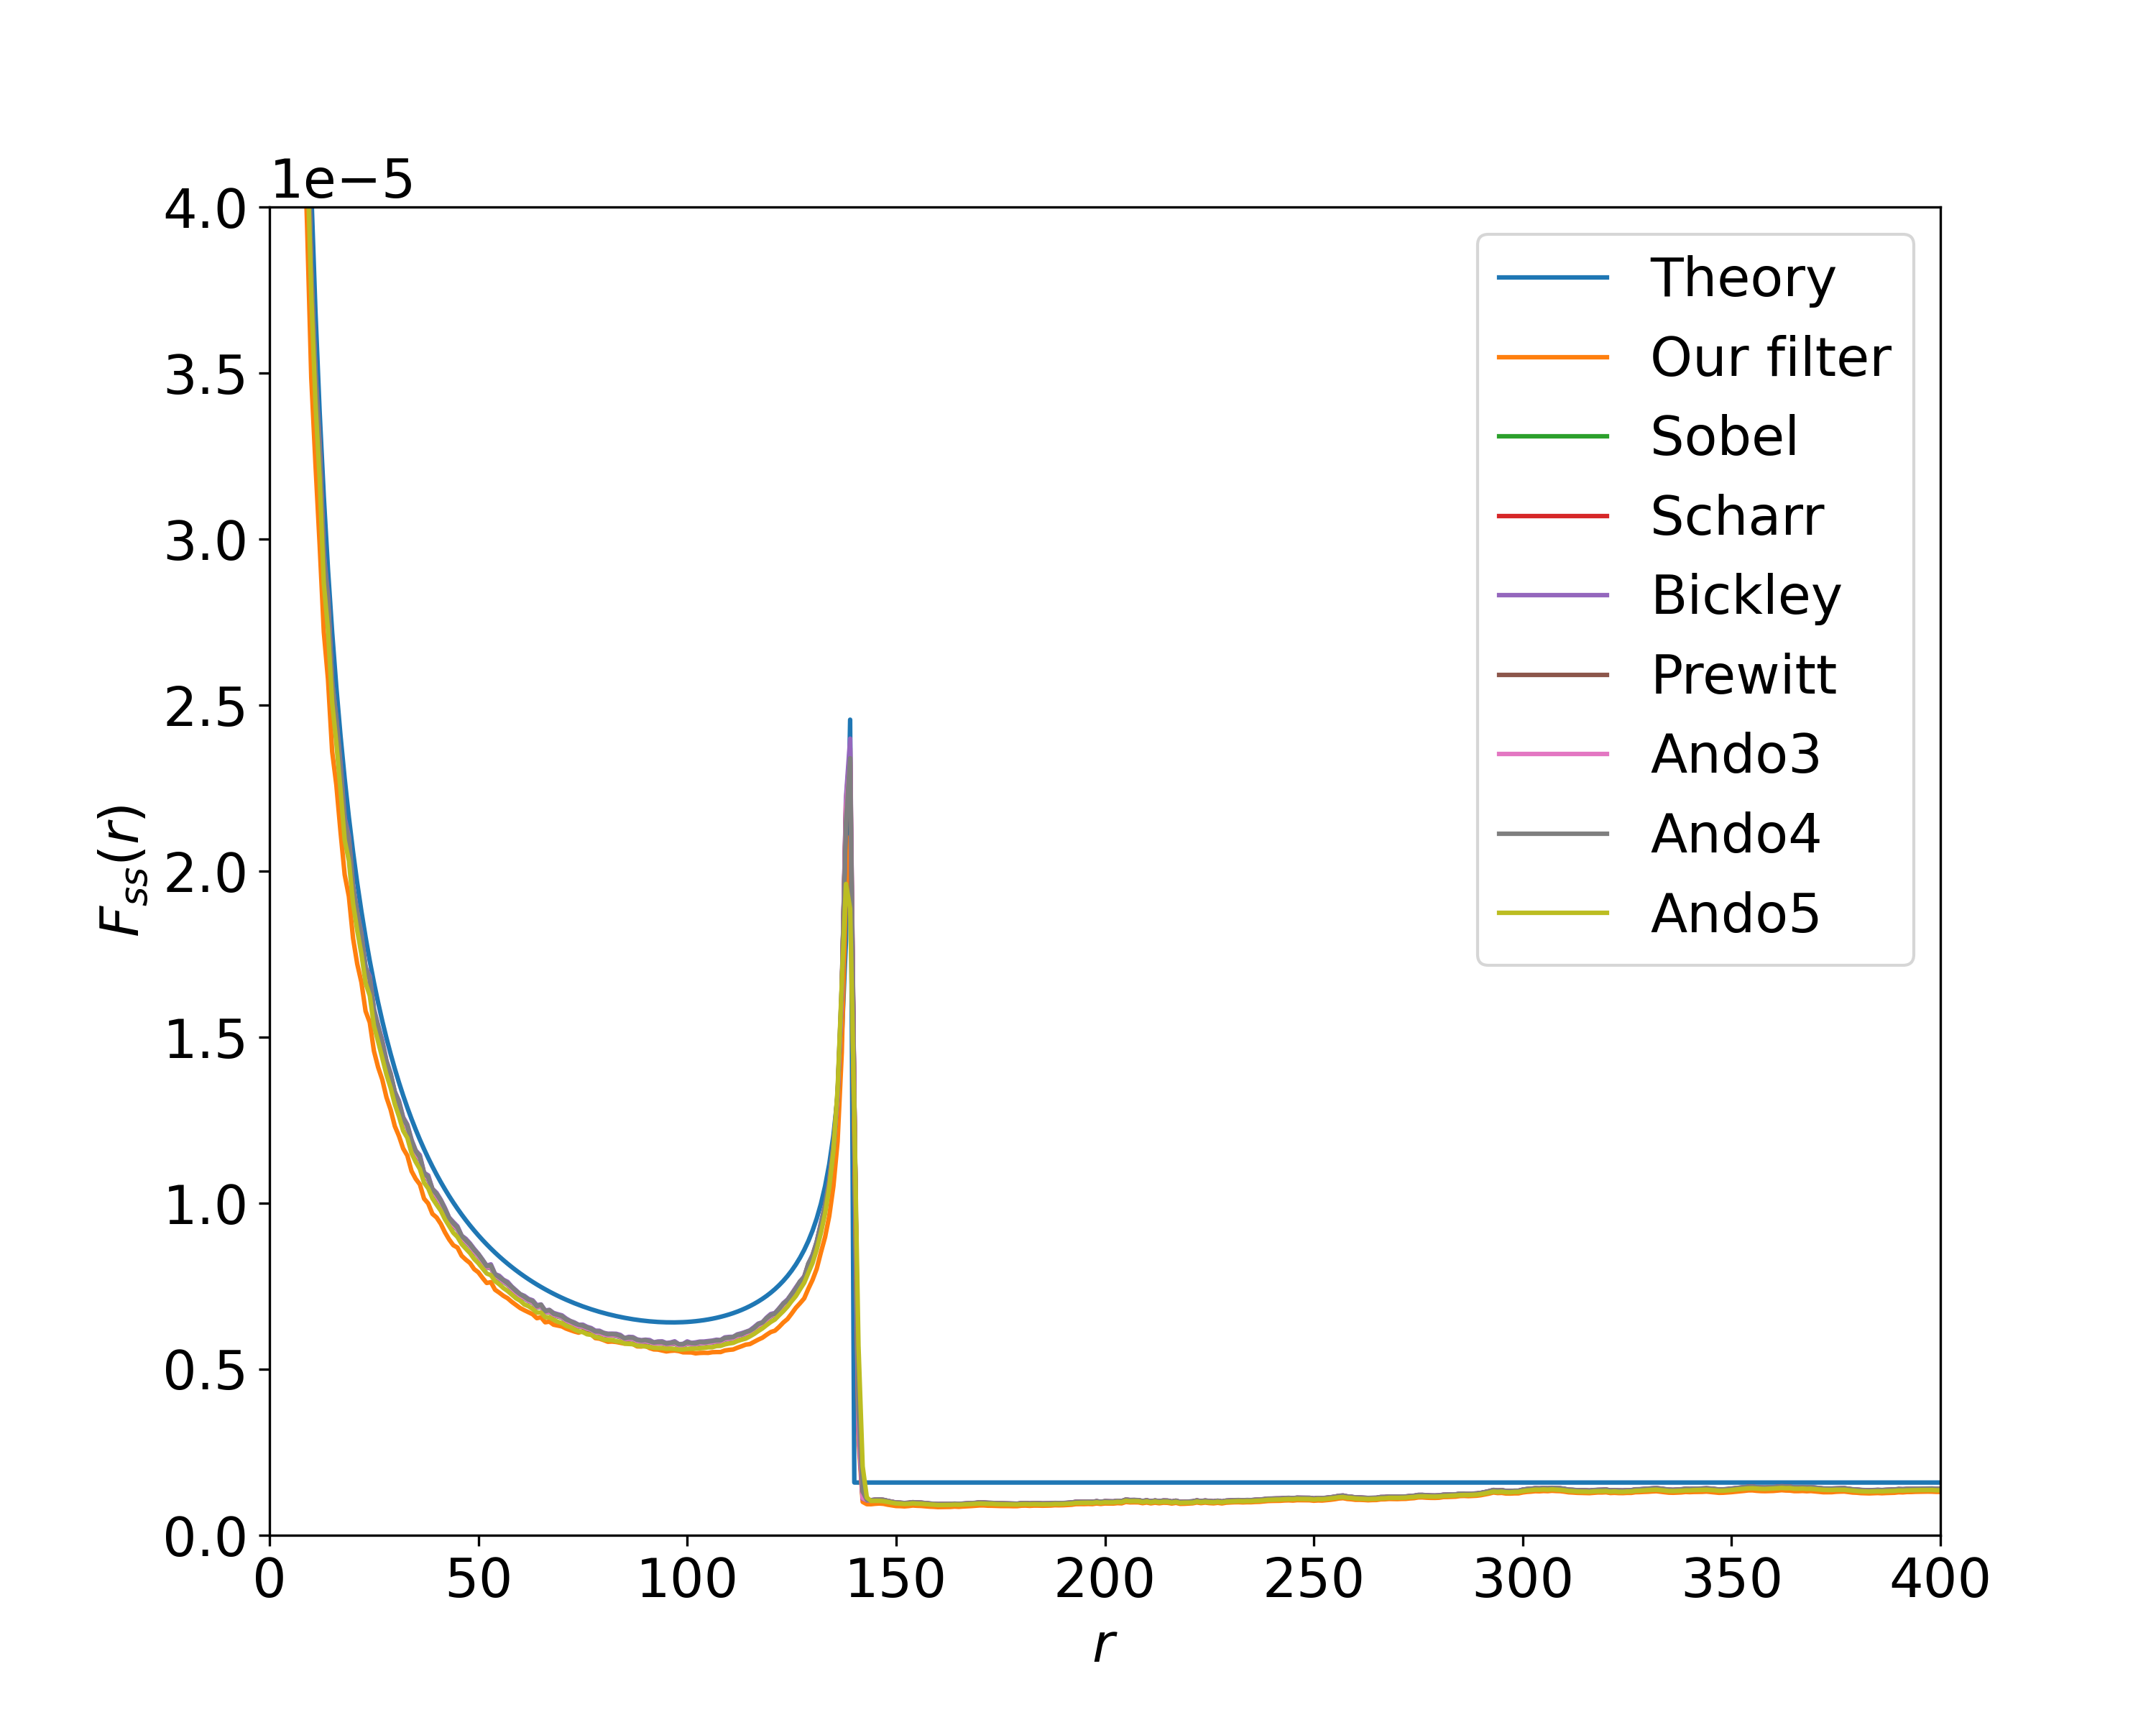
\includegraphics[width=\linewidth]{images/kernels.png}
  \caption{Comparison of different edge-detecting filters in their ability to
    highlight the interface for surface-surface CFs computation (only the case
    of $F_{SS}$ is shown due to similarity of the results for
    $F_{SV}$). \textcolor{red}{input image inset}}
  \label{fig:kernels}
\end{figure}

\section{Application to binary XCT and SEM images of porous media}
\label{sec:application}
After the verification of our computational approach based on analytical
solution and establishing the criterion $C_{0.5}$ we now have enough tools to
evaluate surface CFs for different porous media images, including real XCT and
SEM data.

\subsection{Porous media images collection}
To test our surface CFs computational framework we collected a variety of 3D XCT
and 2D SEM images of two types of natural porous media: sandstones and carbonate
rocks. The fomer are expected to have most of their porosity visible on XCT
scans, expect for nano-porosity associated with the clay that can clog the pore
space. Carbonate rocks are monomineral samples, but usually exhibiting
hierarchical structure, i.e., XCT scanning can reveal only pore sizes with the
range within the imaging resolution, whilst imaging with higher resolution
(e.g., SEM or FIB-SEM techniques) usually reveals sub-micron (under-resolution
porosity for XCT) porosity. The details of the samples are provided in
\textcolor{red}{Table 1}.

\textcolor{red}{Create a table with: Sample name (Sandstone 1... Carbonate 1...;
  Imaging type: XCT or SEM; Dimensions: in pixels/voxels; Imaging resolution:
  $\mu$m; anything else?)}

\textcolor{red}{Are SEM from the same XCT or different samples?}

\subsection{Surface correlation functions for the studied collection}
On \cref{fig:real-data-xct} and \cref{fig:real-data-sem} we report computed
$F_{SS}$ and $F_{SV}$ correlation functions for a variety of XCT and SEM images,
respectively. All these cases satisfy our $C_{0.5}$ criterion and, thus, provide
a possibility to interpret resulting CFs.

\textcolor{red}{We need to interpret the resulting surface CFs somehow - form
  the image i see that for higher resolution $F_{SS}$ seems to be lower, it is
  due to lower desntiy of the interface on higher resolution images? Should we
  compute other corrfunctions, may be even $S_2$ will suffice to further explain
  what happens? Any other ideas on this matter?}

Finally, we show the example of too corase carbonate rock images that fail in
passing the $C_{0.5}$ criterion on \cref{fig:real-bad}. It is possible to apply
the magnification technique to improve $C_{0.5}$, but this lack physical meaning
-- from our experience we can immediately tell that these rocks possess
significant under-resolution porosity that would reveal itself on
higher-resolution images. We discuss the strategies for correct evaluation of
surface correlation functions for such porous media in \cref{sec:outline}.

\begin{figure*}[t]
  \centering
  \subfigure[Sandstone 1, $C_{0.5} = 0.938$]{
    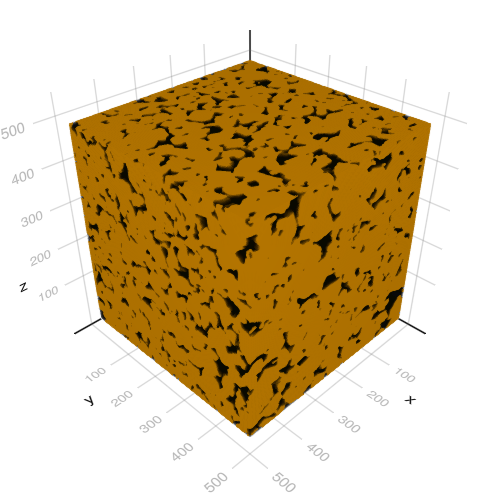
\includegraphics[width=0.14\linewidth, frame]{images/sandstone1.png}
    \label{fig:sandstone1}}
  \hfill
  \subfigure[Sandstone 2, $C_{0.5} = 0.937$]{
    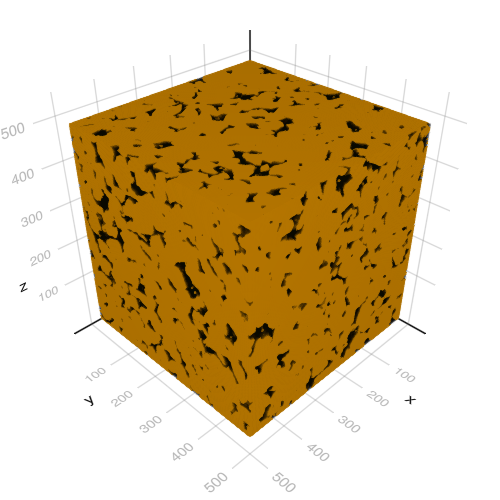
\includegraphics[width=0.14\linewidth, frame]{images/sandstone2.png}
    \label{fig:sandstone2}}
  \hfill
  \subfigure[Sandstone 3, $C_{0.5} = 0.939$]{
    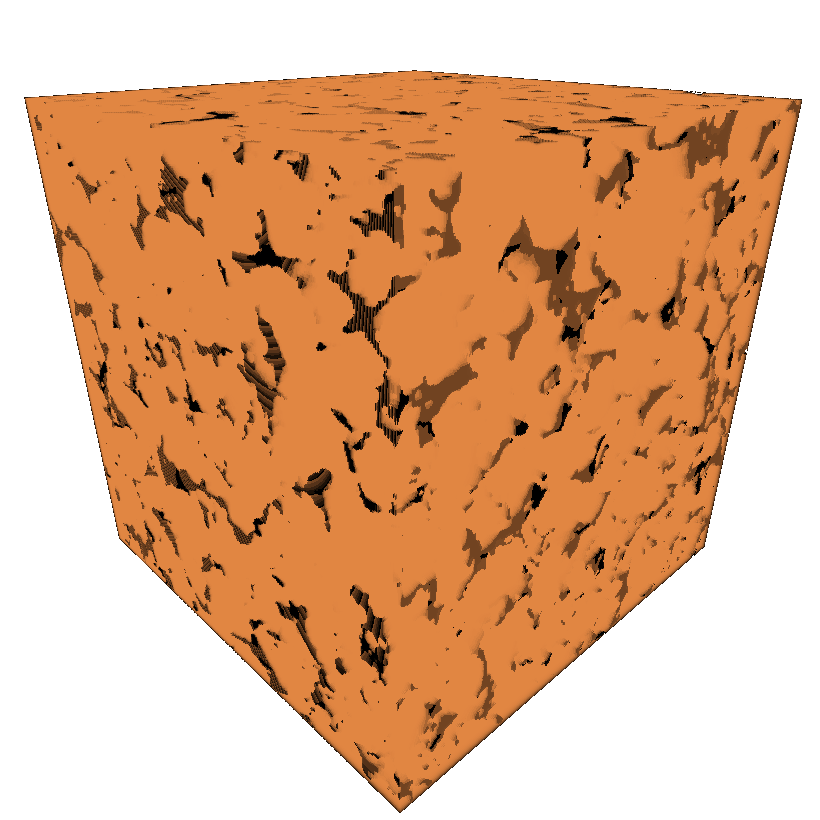
\includegraphics[width=0.14\linewidth, frame]{images/sandstone3.png}
    \label{fig:sandstone3}}
  \hfill
  \subfigure[Carbonate 1, $C_{0.5} = 0.950$]{
    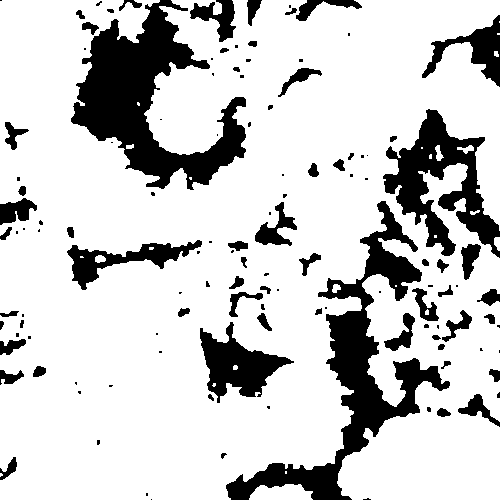
\includegraphics[width=0.14\linewidth, frame]{images/carbonate1.png}
    \label{fig:carbonate1}}
  \hfill
  \subfigure[Carbonate 2, $C_{0.5} = 0.954$]{
    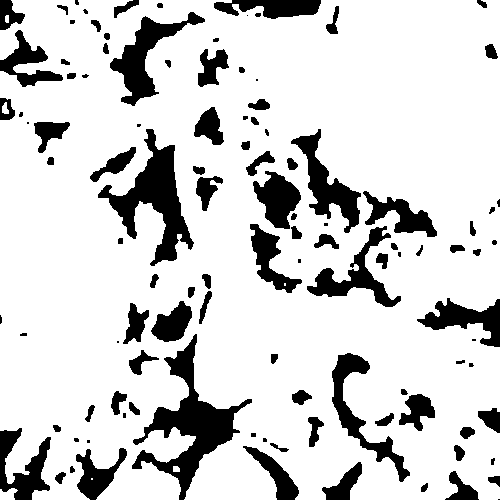
\includegraphics[width=0.14\linewidth, frame]{images/carbonate2.png}
    \label{fig:carbonate2}}
  \hfill
  \subfigure[Carbonate 3, $C_{0.5} = 0.946$]{
    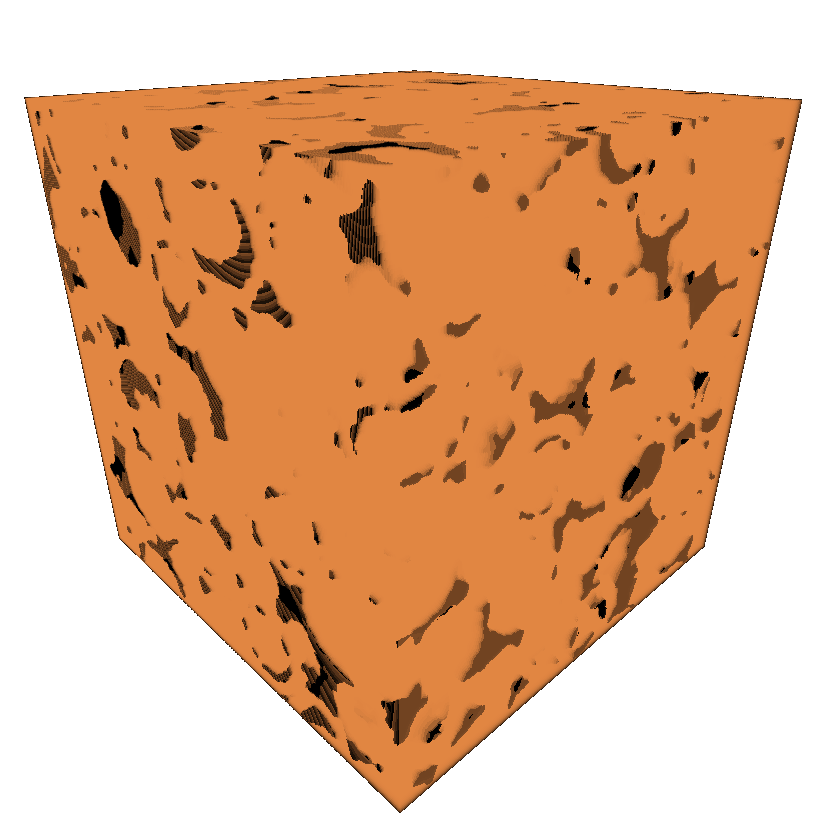
\includegraphics[width=0.14\linewidth, frame]{images/carbonate3.png}
    \label{fig:carbonate3}}
  \vskip\baselineskip
  \subfigure[Surface-surface function]{
    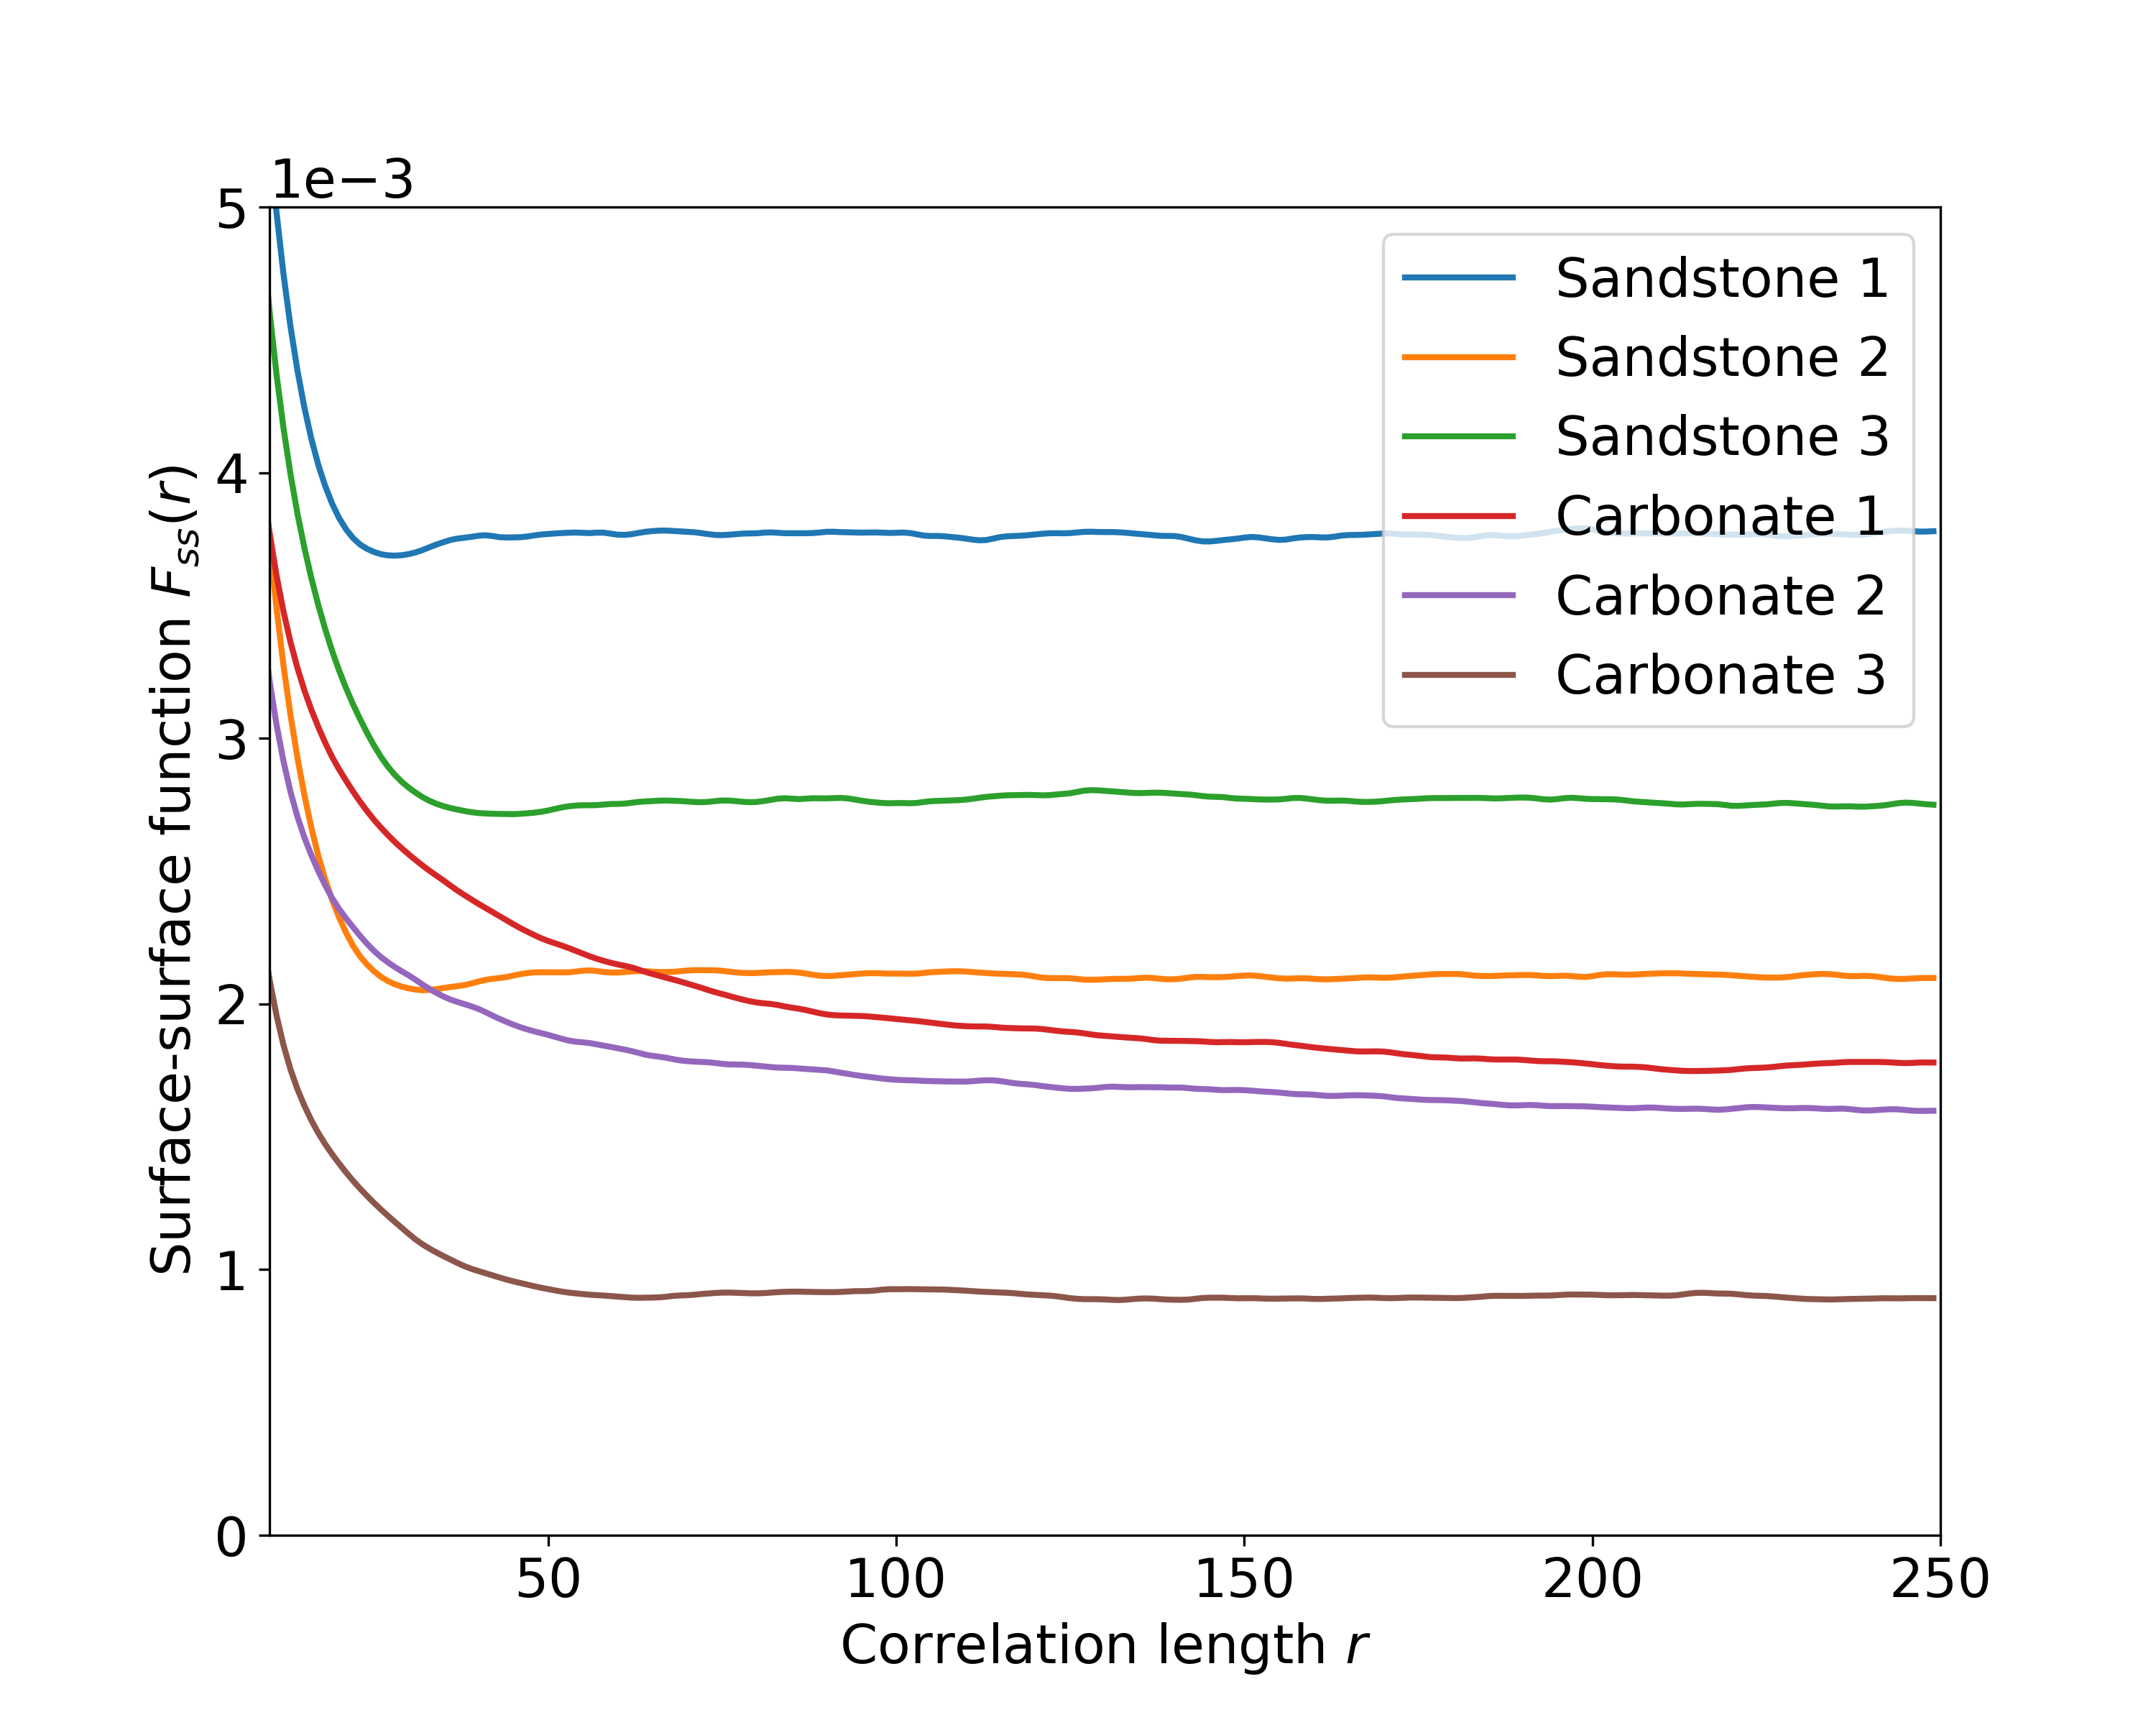
\includegraphics[width=0.475\linewidth]{images/XCT-ss.png}
    \label{fig:plot-ss-real}}
  \hfill
  \subfigure[Surface-void function]{
    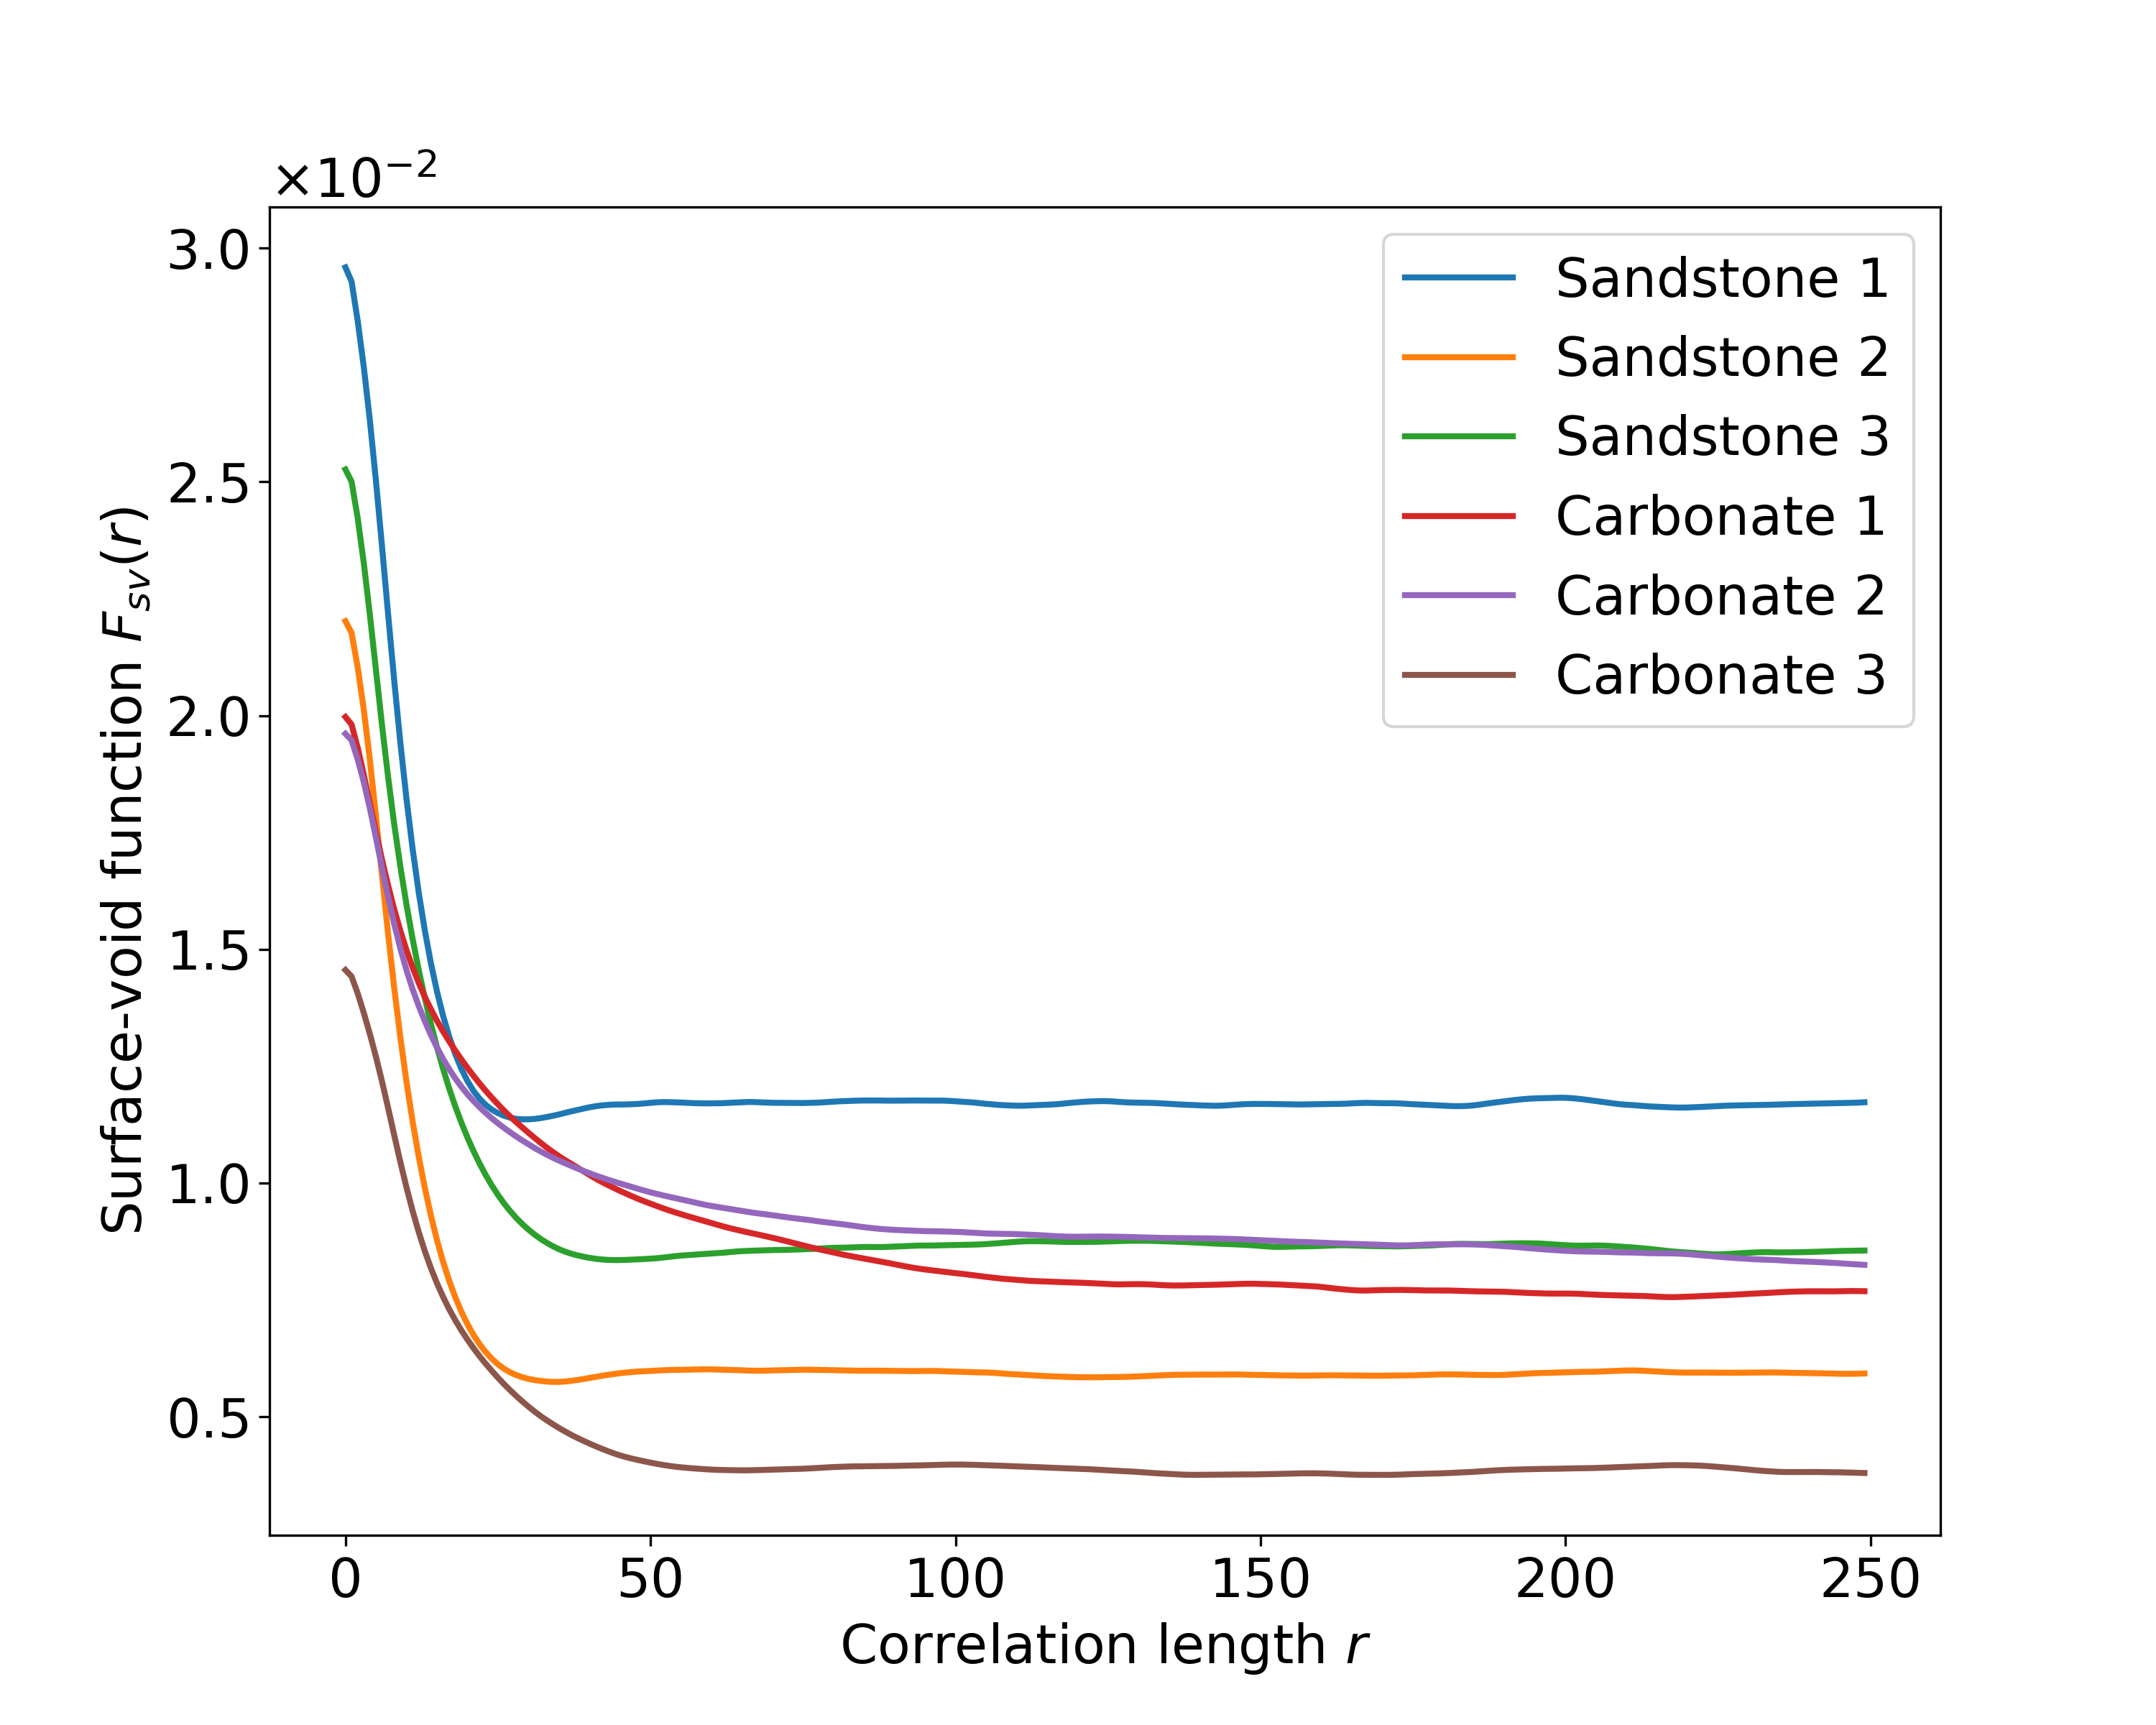
\includegraphics[width=0.475\linewidth]{images/XCT-sv.png}
    \label{fig:plot-sv-real}}
  \caption[]{Examples of XCT images along with surface correlation functions
    calculated using developed methodology. \textcolor{red}{Vasya, please, add
      image frames, we need to add 3d visualizations above the single 2D cut to
      highliht that these are 3D images actually}}
  \label{fig:real-data-xct}
\end{figure*}

\begin{figure*}[t]
  \centering
  \subfigure[Sandstone 4, $C_{0.5} = 0.931$]{
    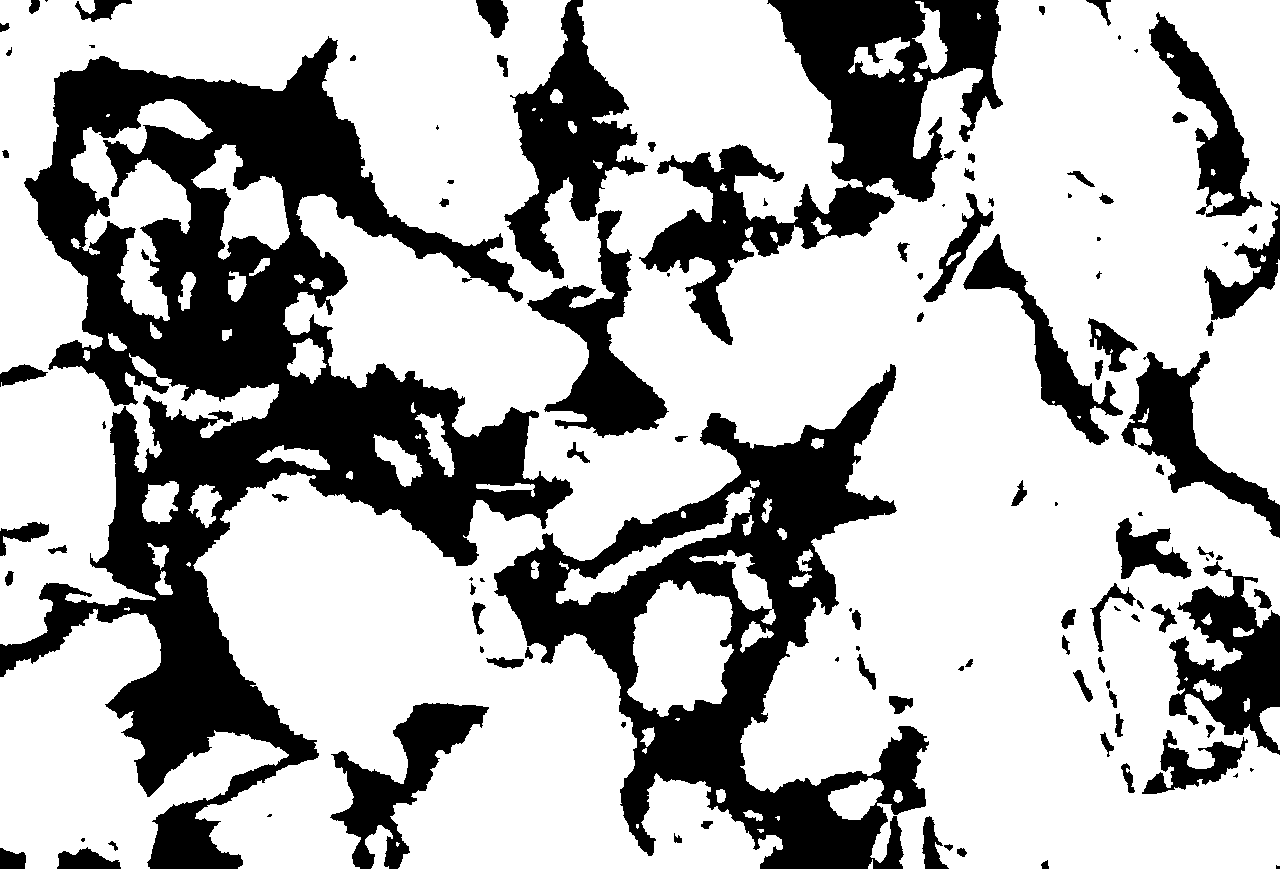
\includegraphics[width=0.2\linewidth, frame]{images/846-79_0009.png}
    \label{fig:sandstone4}}
  \hfill
  \subfigure[Sandstone 5, $C_{0.5} = 0.951$]{
    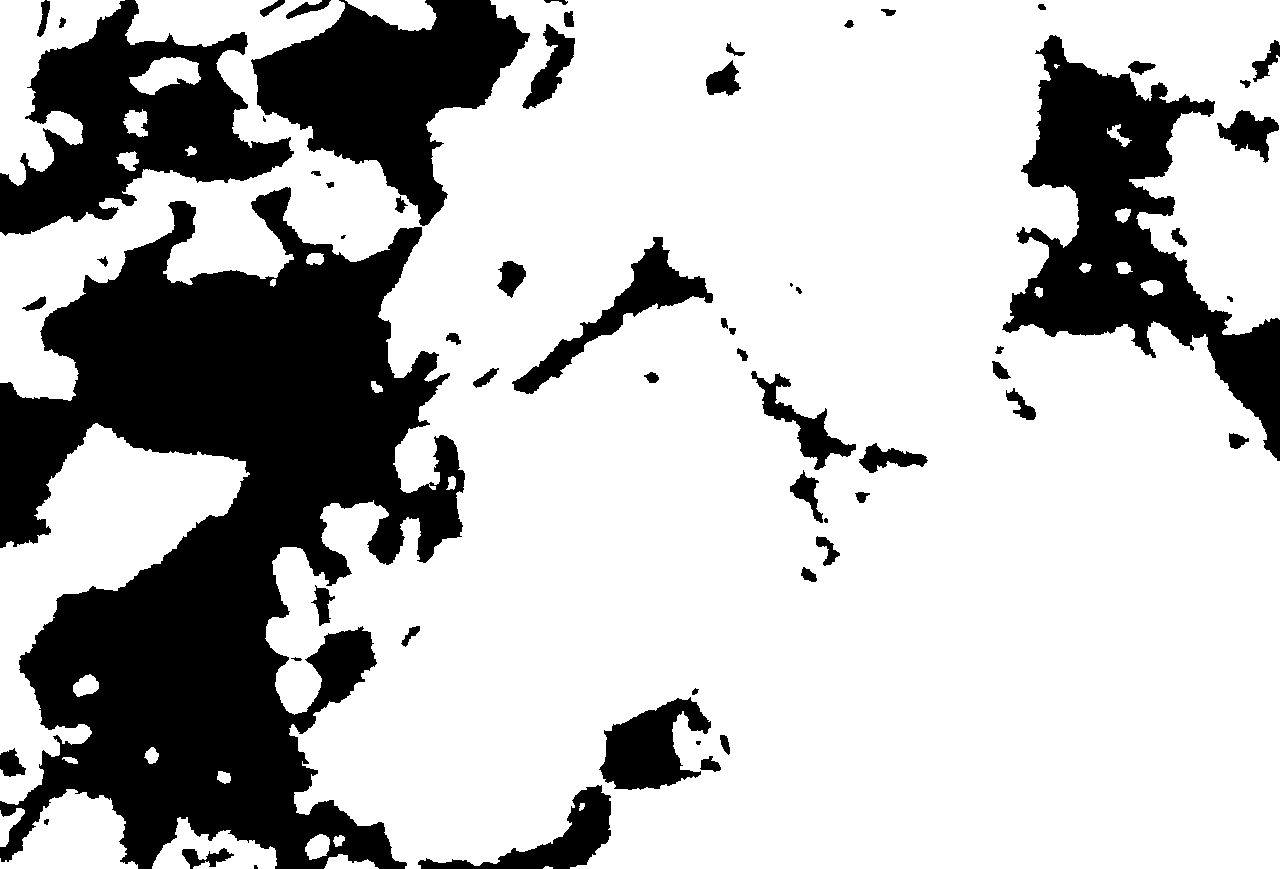
\includegraphics[width=0.2\linewidth, frame]{images/859-12_0005.png}
    \label{fig:sandstone5}}
  \hfill
  \subfigure[Carbonate 4, $C_{0.5} = 0.931$]{
    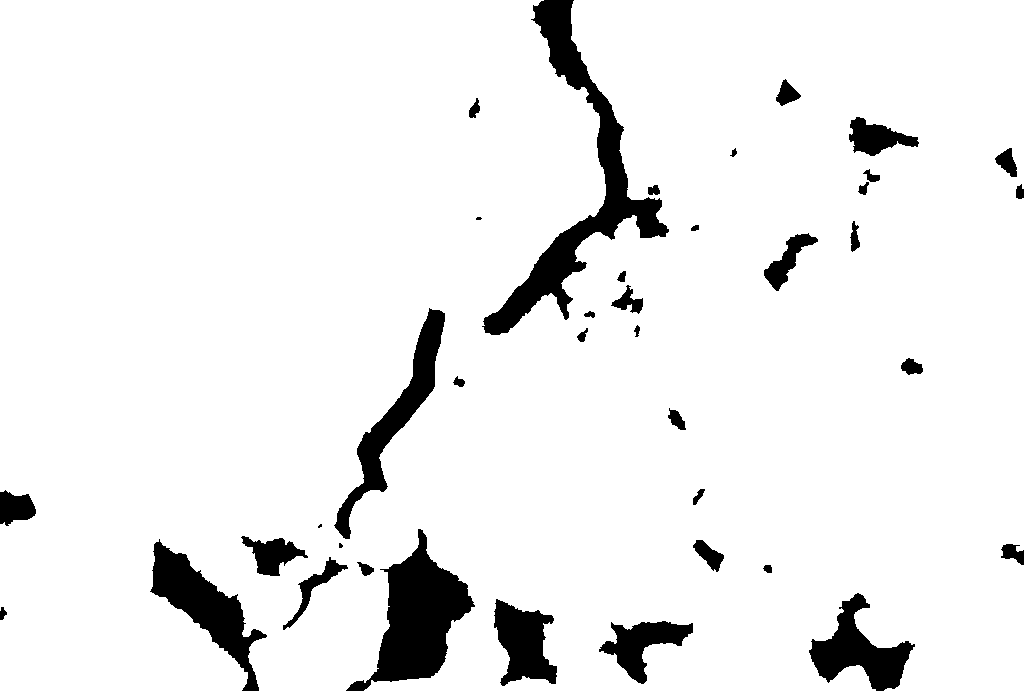
\includegraphics[width=0.2\linewidth, frame]{images/C1-1-g6_010.png}
    \label{fig:carbonate4}}
  \hfill
  \subfigure[Carbonate 5, $C_{0.5} = 0.931$]{
    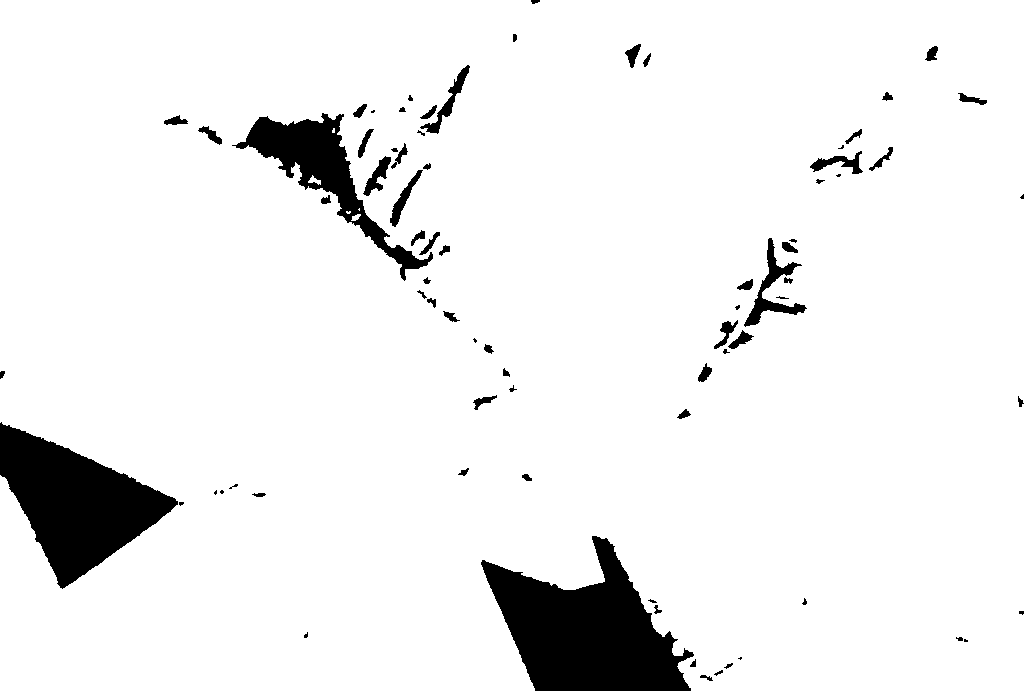
\includegraphics[width=0.2\linewidth, frame]{images/C3-3-G0 (32).png}
    \label{fig:carbonate5}}
  \vskip\baselineskip
  \subfigure[Surface-surface function]{
    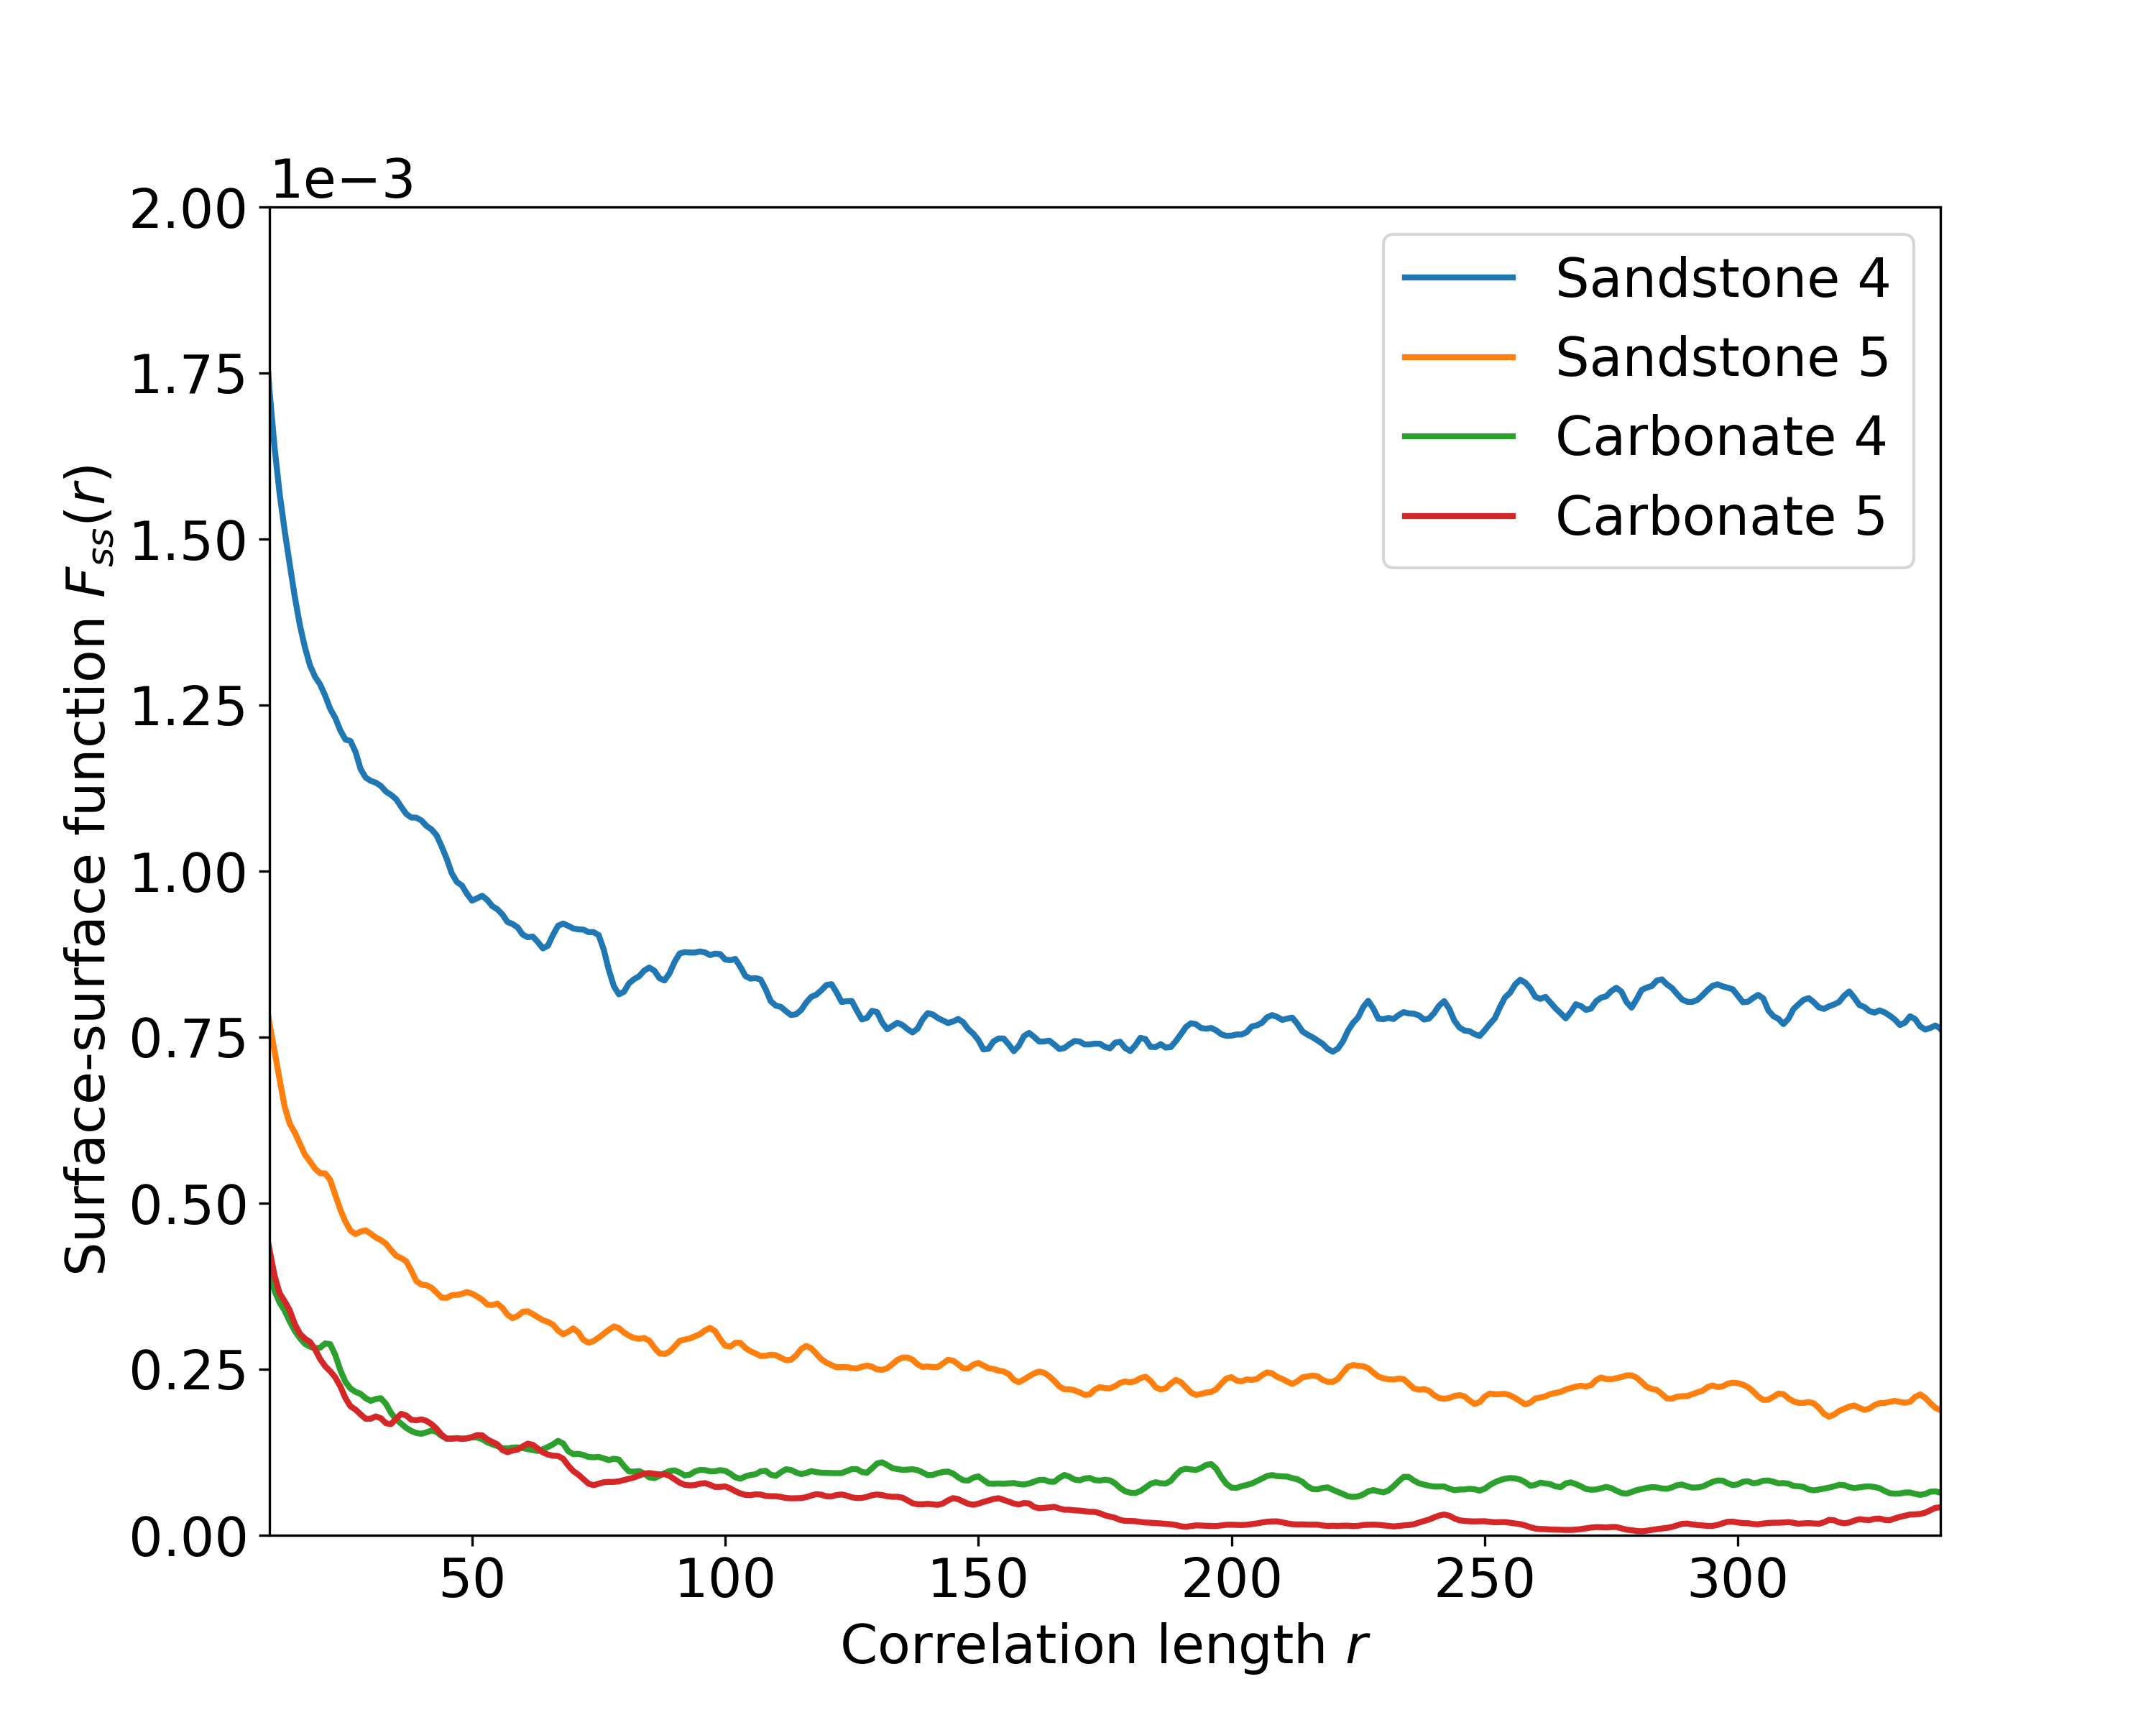
\includegraphics[width=0.475\linewidth]{images/SEM-ss.png}
    \label{fig:plot-ss-real-sem}}
  \hfill
  \subfigure[Surface-void function]{
    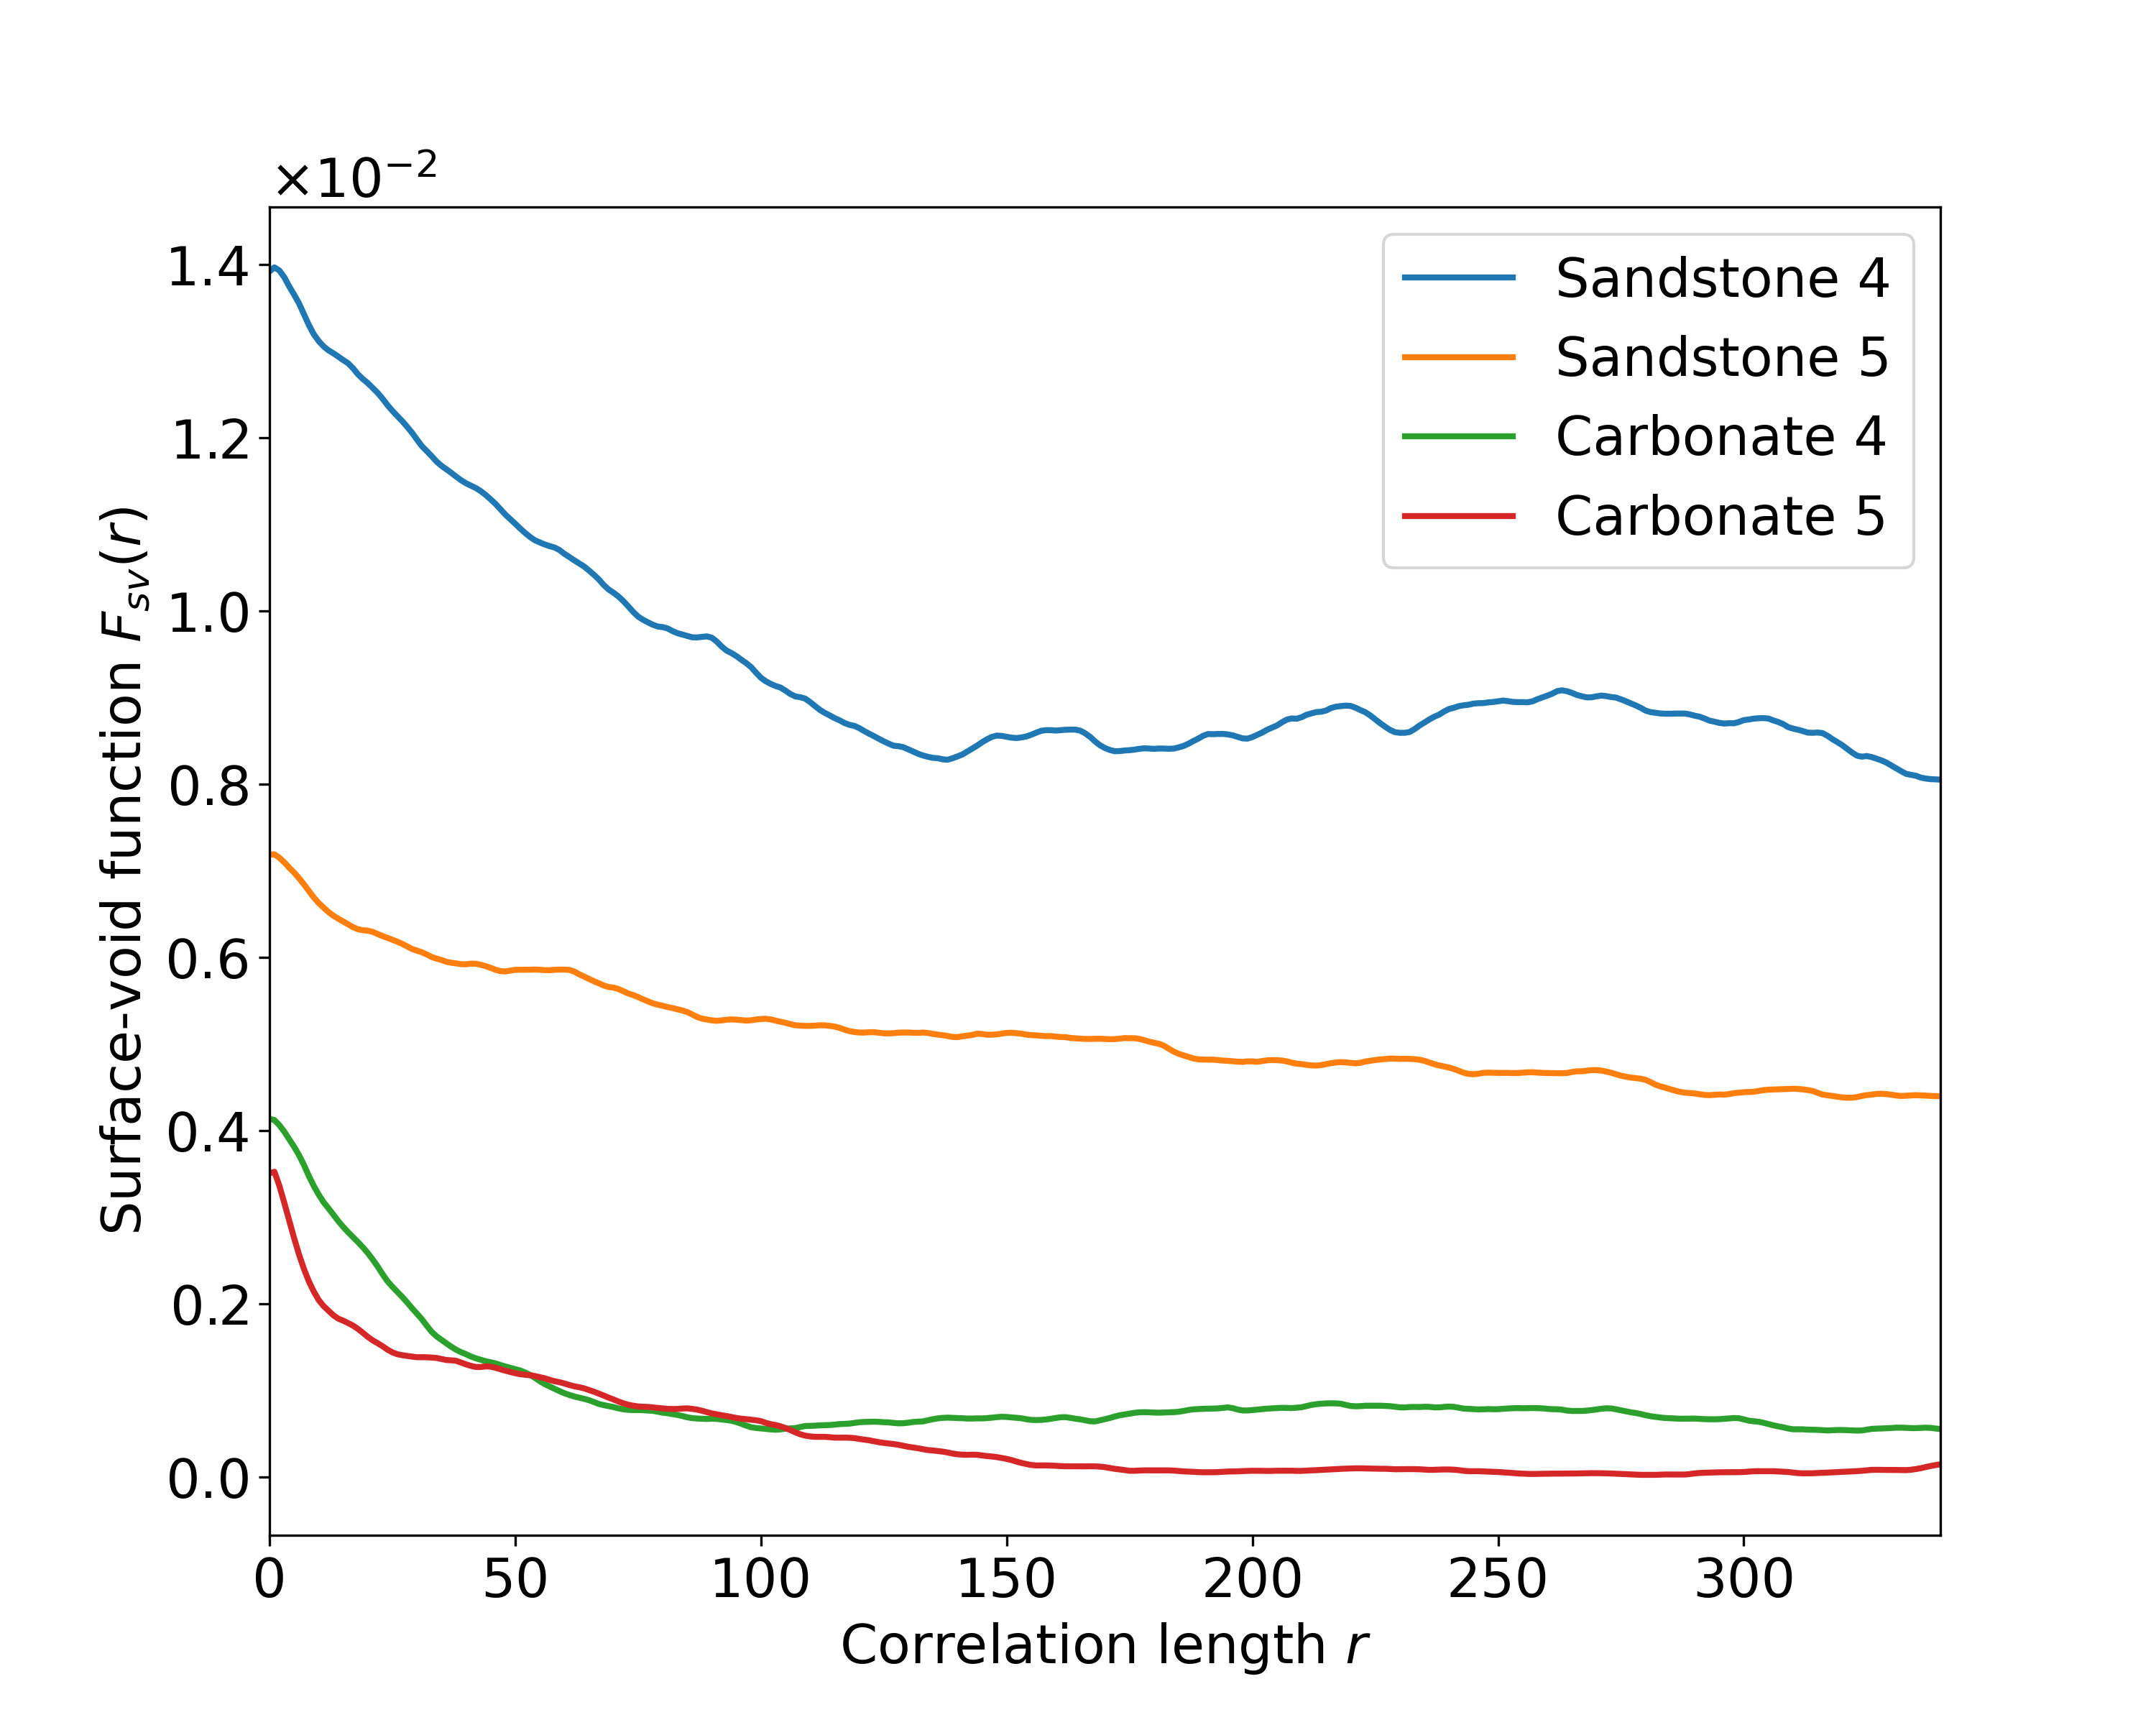
\includegraphics[width=0.475\linewidth]{images/SEM-sv.png}
    \label{fig:plot-sv-real-sem}}
  \caption[]{Examples of surface correlation functions evaluated for SEM images
    of real porous media. \textcolor{red}{add frames for the images, please}}
  \label{fig:real-data-sem}
\end{figure*}

\begin{figure}[t]
  \centering
  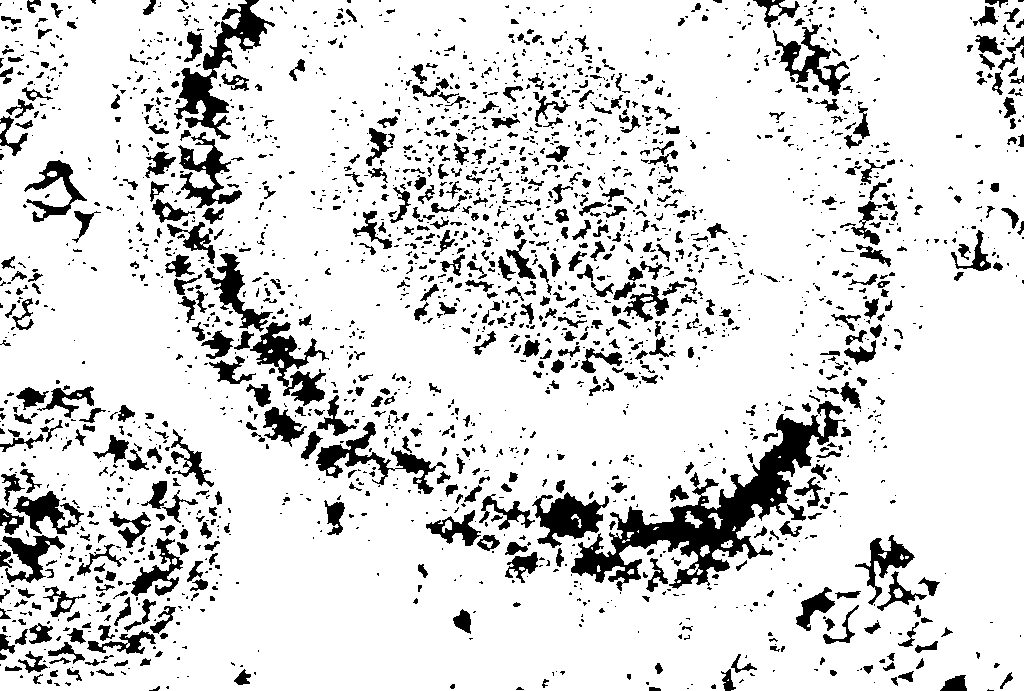
\includegraphics[width=0.475\linewidth]{images/C6-1-2-G2_019.png}
  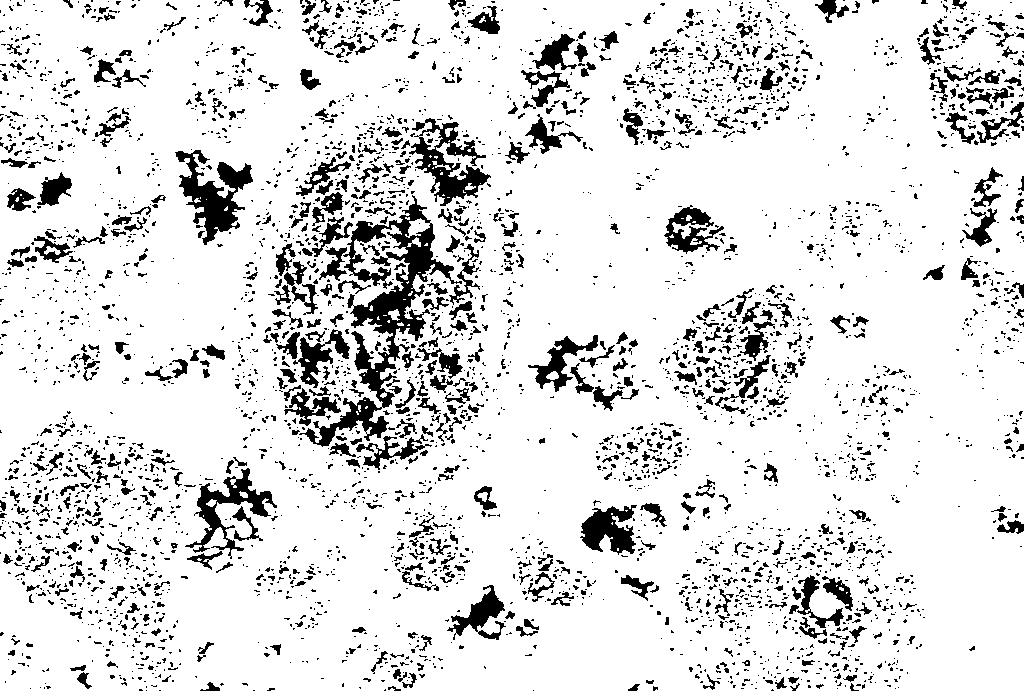
\includegraphics[width=0.475\linewidth]{images/C6-1-2-G2_024.png}
  \caption[]{Examples of carbonate images which do not pass $C_{0.5}$ criterion
    with $C_{0.5} < 0.9$ -- they obviously are of too coarse resolution and
    possess singificant under-resolution porosity. \textcolor{red}{Add that
    those are Carbonate 6 and 7 and their criteria C0.5 like on all previous
    figures}}
  \label{fig:real-bad}
\end{figure}

\subsection{Computational efficiency and robustness}
\textcolor{red}{Report some results for our 2D and 3D samples: CPU and GPU?
  Somewhat briefly is enough. Make CPU and GPU graphs with wall times, including
  the Matlab code for 2D images (we should somehow normilize the results for
  number of segments they sample in their snippet). Compare against the Matlab
  code of Ma and Torquato? May be something like this (feel free to edit and
  improve):}

\textcolor{red}{To demostrate the computational efficicency of our metholody, on
  Fig.X we now report the wall time for surface CFs evaluation for all studied
  images and their sub-croppings. The computations were performed using the
  following workstation running under Linux - specifications - using both CPU
  and GPU computations. The reported elapsed times include the computation of
  the full correlation map and evaluation of the ensemble surface CFs. For 2D
  images we compared wall times against the performance of "continuous" Matlab
  code of Ma and Torquato \cite{ma2018SS}. As expected, our digital approach
  outperforms the "coninuous" method in X orders of magnitude while sampling
  correrlations of all points on the image. Higher sampling rates and the usage
  of edge-detecting filters also improves the robustness of computations, as for
  Poisson disks we obtain values closer to the theoretical ones. Note that we
  provide the code for all computations, as is detailed in \cref{ap:b_code}.}

\section{Discussion and outline}
\label{sec:outline}
Our criterion works only for image without subresolution posity. One can compare
SAS vs. surface CFs to assess invisible interfaces!

Exact vs. for-reconstruction computation of surface CFs

Our way it is easy to implement higher-order statistics computations, such as
multiple-point surface-surface correlation functions.

Discuss super-resolution to improve accuracy of surface functions computation
Explain that ``digital'' is better than ``continuous''.

\section{Summary}
\label{sec:summary}
Our summary says

\section{Acknowledgments}
This research was supported by the Russian Science Foundation grant
19-72-10082.

Collaborative effort of the authors within the FaT iMP (Flow and Transport in
Media with Pores) research group (www.porenetwork.com) and used some of its
software. We thank Prof. Salvatore Torquato for directing us to a
derivation of analytical formulas for 2D Poisson disks. Special thanks goes to
our colleague Dr. Dina Gafurova for the 2D and 3D images of real porous media
used in this study.

\appendix
\section{Derivation of analytical solutions for 2D Poisson disks}
\label{ap:overlapping-disks}
Analytic representation of surface-surface and surface-void correlation
functions for overlapping balls with centers generated by Poisson point process
is well known \cite{Torquato_book}:
\begin{align}
  F_{sv}(r) &= -\lim_{a_1 \rightarrow R} \frac{\partial}{\partial a_1}
  e^{-\lambda S_{tot}(r, a_1, R)} \label{eq:fsv-disks} \\
  F_{ss}(r) &= \lim_{a_1, a_2 \rightarrow R} \frac{\partial}{\partial a_1}
  \frac{\partial}{\partial a_2} e^{-\lambda S_{tot}(r, a_1,
    a_2)} \label{eq:fss-disks}
\end{align}
Here $S_{tot}(r, a_1, a_2)$ refers to a common volume of two n-dimensional balls
of radii $a_1$ and $a_2$ with a distance $r$ between their centers and $\lambda$
is a parameter of Poisson process. For two-dimensional disks we have the
following expression for $S_{tot}(r, a1, a2)$:
\begin{equation}
  S_{tot}(r, a_1, a_2) = \pi a_1^2 + \pi a_2^2 - S_{int}(r, a_1, a_2) \label{eq:total}
\end{equation}
where $S_{int}(r, a_1, a_2)$ is a common area of two disks, being equal to:
\begin{align}
  S_{int}(r, a_1, a_2) =&  a_1^2 \arccos(\frac{r^2+a_1^2-a_2^2}{2a_1r}) + \\
  & a_2^2 \arccos(\frac{r^2+a_2^2-a_1^2}{2a_2r}) - \\
  & \frac{\sqrt{Y}}{2} \label{eq:intersection}
\end{align}
when $r<2R$ and zero otherwise. $Y$ in \cref{eq:intersection} is
\begin{equation*}
  Y = (-r+a_1+a_2)(r+a_2-a_1)(r+a_1-a_2)(r+a_1+a_2)
\end{equation*}
Substituting \cref{eq:intersection} into \cref{eq:total} and then
\cref{eq:total} into \cref{eq:fss-disks} we obtain \cref{eq:fss_final} for
$F_{ss}(r)$.

Similarly substituting \cref{eq:intersection} into \cref{eq:total} and then
\cref{eq:total} into \cref{eq:fsv-disks} we obtain \cref{eq:fsv_final} for
$F_{sv}(r)$.

\section{Implementation of surface function computations}
\label{ap:b_code}
The code used to compute surface correlation functions in this manuscript was
written in Julia language and available as a Jupyter notebook in Supplementary
Materials. It uses \code{CorrelationFunctions.jl} package developed by our group
\cite{CFsjlpaper} that allows efficient computation of surface and other
correlation functions using both CPU and GPU architectures. \textcolor{red}{1)
  add our CF.jl paper and 2) create the Jupyter notebook with the code to submit
  together with the manuscript}

\bibliography{apssamp}
\end{document}
